\documentclass[]{book}
\usepackage{lmodern}
\usepackage{amssymb,amsmath}
\usepackage{ifxetex,ifluatex}
\usepackage{fixltx2e} % provides \textsubscript
\ifnum 0\ifxetex 1\fi\ifluatex 1\fi=0 % if pdftex
  \usepackage[T1]{fontenc}
  \usepackage[utf8]{inputenc}
\else % if luatex or xelatex
  \ifxetex
    \usepackage{mathspec}
  \else
    \usepackage{fontspec}
  \fi
  \defaultfontfeatures{Ligatures=TeX,Scale=MatchLowercase}
\fi
% use upquote if available, for straight quotes in verbatim environments
\IfFileExists{upquote.sty}{\usepackage{upquote}}{}
% use microtype if available
\IfFileExists{microtype.sty}{%
\usepackage{microtype}
\UseMicrotypeSet[protrusion]{basicmath} % disable protrusion for tt fonts
}{}
\usepackage[margin=1in]{geometry}
\usepackage{hyperref}
\hypersetup{unicode=true,
            pdftitle={Workbook: Statistical Thinking for Forensic Practitioners},
            pdfauthor={Sam Tyner, Hal Stern, Alicia Carriquiry, Michael Daniels},
            pdfborder={0 0 0},
            breaklinks=true}
\urlstyle{same}  % don't use monospace font for urls
\usepackage{longtable,booktabs}
\usepackage{graphicx,grffile}
\makeatletter
\def\maxwidth{\ifdim\Gin@nat@width>\linewidth\linewidth\else\Gin@nat@width\fi}
\def\maxheight{\ifdim\Gin@nat@height>\textheight\textheight\else\Gin@nat@height\fi}
\makeatother
% Scale images if necessary, so that they will not overflow the page
% margins by default, and it is still possible to overwrite the defaults
% using explicit options in \includegraphics[width, height, ...]{}
\setkeys{Gin}{width=\maxwidth,height=\maxheight,keepaspectratio}
\IfFileExists{parskip.sty}{%
\usepackage{parskip}
}{% else
\setlength{\parindent}{0pt}
\setlength{\parskip}{6pt plus 2pt minus 1pt}
}
\setlength{\emergencystretch}{3em}  % prevent overfull lines
\providecommand{\tightlist}{%
  \setlength{\itemsep}{0pt}\setlength{\parskip}{0pt}}
\setcounter{secnumdepth}{5}
% Redefines (sub)paragraphs to behave more like sections
\ifx\paragraph\undefined\else
\let\oldparagraph\paragraph
\renewcommand{\paragraph}[1]{\oldparagraph{#1}\mbox{}}
\fi
\ifx\subparagraph\undefined\else
\let\oldsubparagraph\subparagraph
\renewcommand{\subparagraph}[1]{\oldsubparagraph{#1}\mbox{}}
\fi

%%% Use protect on footnotes to avoid problems with footnotes in titles
\let\rmarkdownfootnote\footnote%
\def\footnote{\protect\rmarkdownfootnote}

%%% Change title format to be more compact
\usepackage{titling}

% Create subtitle command for use in maketitle
\newcommand{\subtitle}[1]{
  \posttitle{
    \begin{center}\large#1\end{center}
    }
}

\setlength{\droptitle}{-2em}
  \title{Workbook: Statistical Thinking for Forensic Practitioners}
  \pretitle{\vspace{\droptitle}\centering\huge}
  \posttitle{\par}
  \author{Sam Tyner, Hal Stern, Alicia Carriquiry, Michael Daniels}
  \preauthor{\centering\large\emph}
  \postauthor{\par}
  \date{}
  \predate{}\postdate{}

\usepackage{booktabs}
\usepackage{amsthm}
\makeatletter
\def\thm@space@setup{%
  \thm@preskip=8pt plus 2pt minus 4pt
  \thm@postskip=\thm@preskip
}
\makeatother
\linespread{1.3}

\usepackage{amsthm}
\newtheorem{theorem}{Theorem}[chapter]
\newtheorem{lemma}{Lemma}[chapter]
\theoremstyle{definition}
\newtheorem{definition}{Definition}[chapter]
\newtheorem{corollary}{Corollary}[chapter]
\newtheorem{proposition}{Proposition}[chapter]
\theoremstyle{definition}
\newtheorem{example}{Example}[chapter]
\theoremstyle{remark}
\newtheorem*{remark}{Remark}
\begin{document}
\maketitle

{
\setcounter{tocdepth}{1}
\tableofcontents
}
\chapter{Introduction}\label{introduction}

This workbook is intended to accompany the Statistical Thinking for
Forensic Practitioners workshop taught by members of the Center for
Statistics and Applications in Forensic Evidence (CSAFE). The slides for
this workshop were constructed by Hal Stern, Alicia Carriquiry, and
Michael Daniels.

When taking the workshop, please follow along with the slides handout
(if given) and this workbook. The workbook contains the same material as
the slides, with room for you to take notes and to fill in the missing
material.

\chapter{Statistical Preliminaries}\label{statistical-preliminaries}

Briefly, this section contains a broad review of probability concepts
and of statistical inference concepts, with examples from the forensic
science context. We will cover probability, data collection, statistical
distributions, estimation, and hypothesis testing. \vspace{-.25in}

\subsection{Definitions}\label{definitions}

\begin{itemize}
\tightlist
\item
  \textbf{population}:
  \_\_\_\_\_\_\_\_\_\_\_\_\_\_\_\_\_\_\_\_\_\_\_\_\_\_\_\_\_\_\_\_\_\_\_\_\_\_\_\_\_\_\_\_\_\_\_\_\_\_\_\_\_\_
\end{itemize}

\vspace{.1in}

\begin{itemize}
\tightlist
\item
  \textbf{sample}:
  \_\_\_\_\_\_\_\_\_\_\_\_\_\_\_\_\_\_\_\_\_\_\_\_\_\_\_\_\_\_\_\_\_\_\_\_\_\_\_\_\_\_\_\_\_\_\_\_\_\_\_\_\_
\end{itemize}

\vspace{.1in}

\begin{itemize}
\tightlist
\item
  \textbf{probability}: Using knowledge about the
  \_\_\_\_\_\_\_\_\_\_\_\_\_\_\_\_ to make statements describing the
  \_\_\_\_\_\_\_\_\_\_\_\_\_\_\_\_\_\_. Probability can loosely be
  thought of as a type of deductive reasoning, where we are applying
  general knowledge about the population of interest to make conclusions
  about a small part of that population.
\end{itemize}

\vspace{.1in}

\begin{itemize}
\tightlist
\item
  \textbf{statistics}: Using knowledge about the
  \_\_\_\_\_\_\_\_\_\_\_\_\_\_\_\_ to make statements describing the
  \_\_\_\_\_\_\_\_\_\_\_\_\_\_\_\_\_\_. Statistics can loosely be
  thought of as a type of inductive reasoning, where we are applying
  knowledge about a sample to state that something \emph{may} be true
  about the population generally.
\end{itemize}

\begin{figure}[h]

{\centering 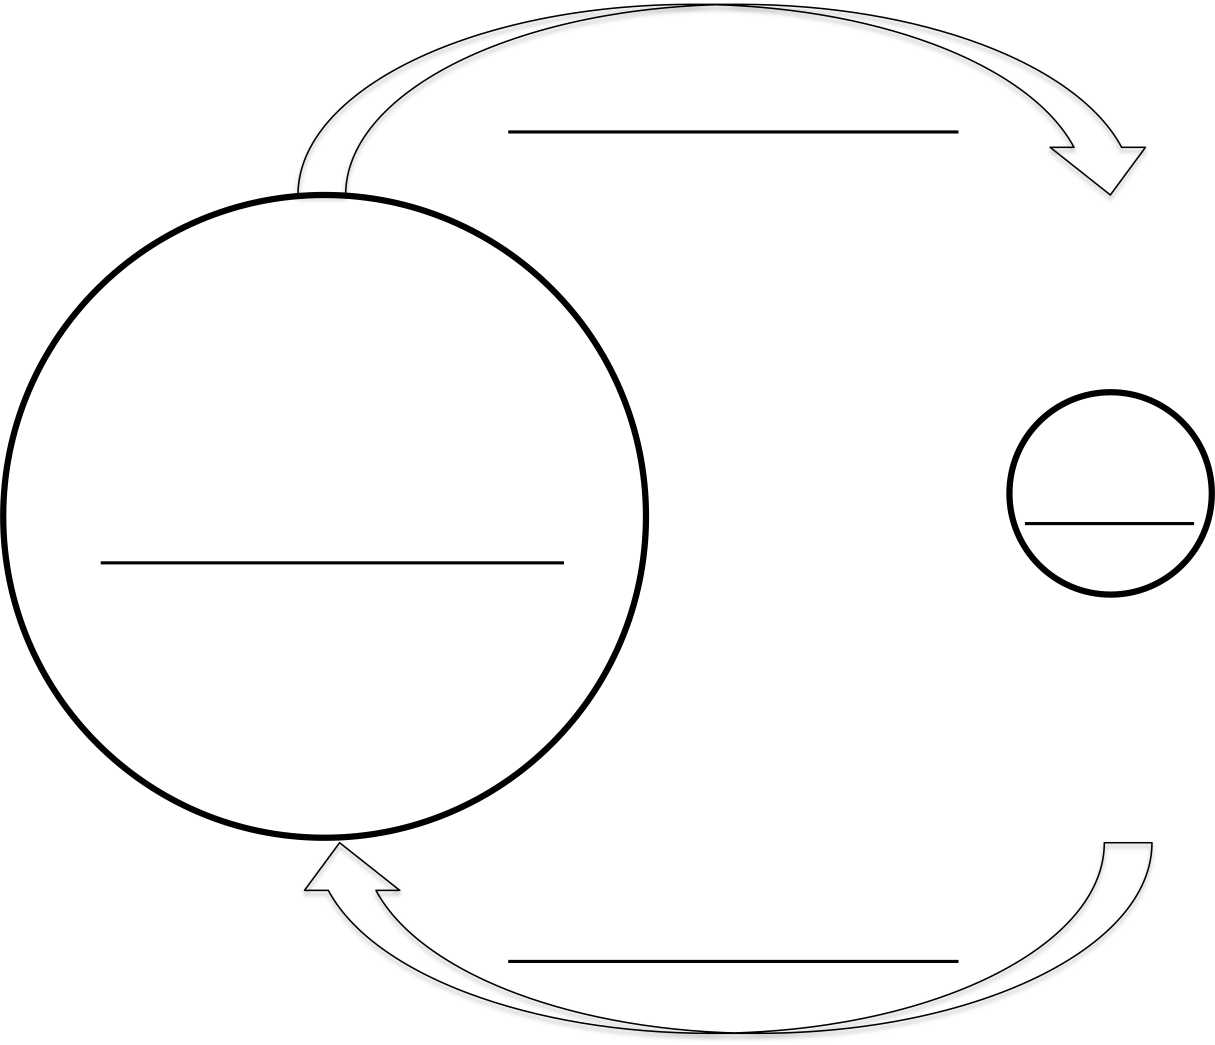
\includegraphics[width=.5\linewidth]{img/thebigpic} 

}

\caption{"The Big Picture"}\label{fig:thebigpic}
\end{figure}

\subsection{Forensic Science Examples}\label{forensic-science-examples}

\begin{itemize}
\tightlist
\item
  Suppose 100 1-pound bags of heroin are seized on the US-Mexico border,
  and the FBI want to know the chemical composition of the confiscated
  drugs to store in their database.\vspace{.1in}

  \begin{itemize}
  \tightlist
  \item
    Population: \_\_\_\_\_\_\_\_\_\_\_\_\_\_\_\_\_\_\_\_\_\_\_\_\_\_
    \vspace{.1in}
  \item
    Sample: \_\_\_\_\_\_\_\_\_\_\_\_\_\_\_\_\_\_\_\_\_\_\_\_\_\_
    \vspace{.1in}
  \end{itemize}
\item
  A window was broken in a robbery, and the suspect who was apprehended
  nearby had glass fragments lodged in the soles of their shoes. Do the
  fragments from the suspect's shoes have the same or similar chemical
  composition as the broken window? \vspace{.1in}

  \begin{itemize}
  \tightlist
  \item
    Population 1: \_\_\_\_\_\_\_\_\_\_\_\_\_\_\_\_\_\_\_\_\_\_\_\_\_\_
    \vspace{.1in}
  \item
    Sample 1: \_\_\_\_\_\_\_\_\_\_\_\_\_\_\_\_\_\_\_\_\_\_\_\_\_\_\\
    \vspace{.1in}
  \item
    Population 2: \_\_\_\_\_\_\_\_\_\_\_\_\_\_\_\_\_\_\_\_\_\_\_\_\_\_
    \vspace{.1in}
  \item
    Sample 2: \_\_\_\_\_\_\_\_\_\_\_\_\_\_\_\_\_\_\_\_\_\_\_\_\_\_\\
    \vspace{.1in}
  \end{itemize}
\item
  A city government employee is suspected of embezzling funds from the
  city's coffers. Forensic accountants examine a subset of the city's
  transactions to determine whether embezzling occurred and how much
  money was lost. \vspace{.1in}

  \begin{itemize}
  \tightlist
  \item
    Population: \_\_\_\_\_\_\_\_\_\_\_\_\_\_\_\_\_\_\_\_\_\_\_\_\_\_
    \vspace{.1in}
  \item
    Sample: \_\_\_\_\_\_\_\_\_\_\_\_\_\_\_\_\_\_\_\_\_\_\_\_\_\_
  \end{itemize}
\end{itemize}

How do you think this pertains to pattern evidence? List some possible
relevant populations and samples below.\vspace{.1in}

\begin{itemize}
\tightlist
\item
  Population 1: \_\_\_\_\_\_\_\_\_\_\_\_\_\_\_\_\_\_\_\_\_\_\_\_\_\_
  \vspace{.1in}
\item
  Sample 1: \_\_\_\_\_\_\_\_\_\_\_\_\_\_\_\_\_\_\_\_\_\_\_\_\_\_\\
  \vspace{.1in}
\item
  Population 2: \_\_\_\_\_\_\_\_\_\_\_\_\_\_\_\_\_\_\_\_\_\_\_\_\_\_
  \vspace{.1in}
\item
  Sample 2: \_\_\_\_\_\_\_\_\_\_\_\_\_\_\_\_\_\_\_\_\_\_\_\_\_\_
  \vspace{.1in}
\item
  Population 3: \_\_\_\_\_\_\_\_\_\_\_\_\_\_\_\_\_\_\_\_\_\_\_\_\_\_
  \vspace{.1in}
\item
  Sample 3: \_\_\_\_\_\_\_\_\_\_\_\_\_\_\_\_\_\_\_\_\_\_\_\_\_\_
\end{itemize}

\section{Probability}\label{probability}

Probability concerns the \emph{uncertainty} of outcomes. The set of all
possible outcomes is called the \_\_\_\_\_\_\_\_\_\_\_ space, and a
particular outcome or set of outcomes of interest is referred to as an
\_\_\_\_\_\_\_\_\_\_.

\subsection{Examples}\label{examples}

\begin{enumerate}
\def\labelenumi{\arabic{enumi}.}
\tightlist
\item
  Footwear

  \begin{itemize}
  \tightlist
  \item
    Sample Space = All shoe sizes e.g.
    \(\{6, 6.5, 7, 7.5, 8, 8.5, \dots\}\)
  \item
    Event = Shoe of size 9
  \end{itemize}
\item
  Footwear

  \begin{itemize}
  \tightlist
  \item
    Sample Space = Brand of shoe e.g. \{ Nike, Vans, Converse,
    \(\dots\)\}
  \item
    Event = Nike sneaker
  \end{itemize}
\item
  Firearms

  \begin{itemize}
  \tightlist
  \item
    Sample Space = CMS (consecutive matching striae) for a pair of
    bullets e.g. \(\{0, 1, 2, 3, 4, \dots \}\)
  \item
    Event = CMS of 10 or more
  \end{itemize}
\end{enumerate}

\subsection{Interpretation}\label{interpretation}

The probability of observing an event in a sample space is a number less
than or equal to 1 and greater than or equal to 0 that describes the
\_\_\_\_\_\_\_\_\_\_\_\_ that the event will occur.

There are two primary interpretations of probability: \vspace{.1in}

\begin{enumerate}
\def\labelenumi{\arabic{enumi}.}
\tightlist
\item
  The long run \_\_\_\_\_\_\_\_\_\_\_\_ of occurrence of an event.
  \vspace{.1in}
\item
  The \_\_\_\_\_\_\_\_\_\_\_\_\_ belief of likelihood of an event
  occurring.
\end{enumerate}

\subsection{Basic Notation and Laws of
Probability}\label{basic-notation-and-laws-of-probability}

Let an event of interest be denoted by \_\_\_\_\_\_\_. The probability
of this event occurring is then denoted \_\_\_\_\_\_\_\_\_\_. Recall
that the probability of an event is always between 0 and 1. When
\(P(Y) = 0\), the event \(Y\) will never happen. When \(P(Y) = 1\), the
event \(Y\) will always happen. The sum of the probabilities of all
possbile outcomes in the sample space always equal to \_\_\_\_\_.

The event of interest, \(Y\), also has a complement event,
\(\overline{Y}\), which is read as ``not \(Y\)''. The complement,
\(\overline{Y}\), of an event, \(Y\), is itself an event containing all
outcomes in the sample space other than that initial event of interest,
\(Y\).

\[ P(Y) + P(\overline{Y}) = \_\_\_\]

The above equation also gives us the following rules:

\begin{equation}\label{eq:1}
\begin{split}
P(Y) & = 1 - P(\overline{Y}) \\
 P(\overline{Y}) & = 1 - P(Y)
\end{split}
\end{equation}

\subsection{Probability and Odds}\label{probability-and-odds}

The probability of an event defines the odds of the event. The odds
\emph{in favor} of an event \(Y\) are defined as the probability of
\(Y\) divided by the probability of everything except \(Y\) (``not
\(Y\)''):

\[ O(Y) = \dfrac{P(Y)}{P(\overline{Y})} = \dfrac{P(Y)}{1-\_\_}.\]

Conversely, the odds \emph{against} a event \(Y\) are defined as the
probability of everything except \(Y\) (``not \(Y\)'') divided by the
probability of \(Y\):

\[ O(\overline{Y}) = \dfrac{P(\overline{Y})}{P(Y)} = \dfrac{1-\_\_}{P(Y)}.\]

When we typically talk about odds, like in horse racing, the odds
reported are the odds \emph{against} the outcome of interest. Let's
construct a horse race scenario using our probability notation to find
the probability of a horse winning a race from the reported odds:

\begin{itemize}
\tightlist
\item
  Suppose you want to place a bet on a horse name Cleopatra winning the
  race. Odds for Cleopatra are reported as 4:1.
\item
  \(Y\) = Cleopatra wins the race
\item
  \(\overline{Y}\) = Any horse in the race \emph{other than} Cleopatra
  wins the race.
\item
  \(O(\overline{Y}) = \dfrac{P(\overline{Y})}{P(Y)} = \frac{4}{1} = 4\)
\item
  We know that \(P(Y) + P(\overline{Y})=1\). With this information, we
  can determine \(P(Y)\), which is the probability that Cleopatra wins
  the race:

  \begin{align*}
  O(\overline{Y}) & = \dfrac{P(\overline{Y})}{P(Y)} = 4 \\
  \Rightarrow  \dfrac{P(\overline{Y})}{P(Y)} & = 4 \\ \Rightarrow  \dfrac{1 - P(Y)}{P(Y)} & = 4 \quad \quad \textit{(See Equation \ref{eq:1})} \\ 
  \Rightarrow \dfrac{1}{P(Y)} - 1 & = 4 \\
  \Rightarrow \dfrac{1}{P(Y)} & = 5 \\
  \Rightarrow P(Y) & = \frac{1}{5} = 0.2 \\
  \Rightarrow P(\overline{Y}) & = 0.8
  \end{align*}
\item
  So, the odds for Cleopatra (4:1) mean that Cleopatra has a probability
  of 0.2 of winning the race. Because this outcome is not very likely
  (it will only happen in 1 race out of 5), you win money if Cleopatra
  wins simply because that is not a likely outcome.
\item
  \textbf{Betting}: Suppose you bet \$1 on Cleopatra to win the race
  with 4:1 odds. You will win \$4 if Cleopatra wins, otherwise you've
  lost \$1.
\item
  The amount you win (\$4) is determined so that you break even in the
  long run.
\item
  Suppose 5 identical races are run. In 1 of those races, Cleopatra will
  win, and in the other 4, Cleopatra will lose. If you bet \$1 on
  Cleopatra in each race, you will lose that \$1 4 of 5 times. So, in
  order for you to break even, the designated amount you'll win when
  Cleopatra wins is \$4.
\item
  This is a statistical concept known as \emph{expected value}. Your
  expected value when placing the bet is \$0. We compute expected value
  by multiplying each possible outcome value by its probability and
  adding them all together:

  \begin{align*}
  \$4\cdot P(Y) + (-\$1) \cdot P(\overline{Y}) & = 0 \\
  \$4\cdot 0.2 + (-\$1) \cdot 0.8 & = 0 \\
  \$0.8 - \$0.8 & = 0
  \end{align*}
\end{itemize}

\subsection{Probability Math}\label{probability-math}

Up until now, we have only considered one event, \(Y\). Now, suppose we
have another event that we are interested in, \(Z\).

Let's consider the possibility of \emph{either} of these two events,
\(Y\) or \(Z\), occurring. We'd write this as \(Y \cup Z\), which is
mathematical notation for ``\(Y\) or \(Z\) occurs''. There are two
scenarios that arise: \vspace{.1in}

\begin{enumerate}
\def\labelenumi{\arabic{enumi}.}
\tightlist
\item
  \(Y\) and \(Z\) cannot occur together: they are \_\_\_\_\_\_\_\_\_
  \_\_\_\_\_\_\_\_\_\_ \vspace{.1in}
\item
  \(Y\) and \(Z\) can occur together.
\end{enumerate}

In scenario \#1, computing the probability of either \(Y\) or \(Z\)
happening is easy: we just add their respective probabilities together:

\[ Y,Z \text{ mutually exclusive } \Rightarrow P(Y \cup Z) = P(Y) + P(Z)\]

In scenario \#2, computing the probability of either \(Y\) or \(Z\)
happening is more complicated because we know there is a chance that
\(Y\) and \(Z\) can happen together. We'd write this as \(Y \cap Z\),
which is mathematical notation for ``\(Y\) and \(Z\) occurs''. In
scenario \#1, this event never occurred, so \(P(Y \cap Z) = 0\) there.
To compute the probability of \(Y\) or \(Z\) occurring in scenario \#2,
we have to consider the probability of \(Y\), the probability of \(Z\),
and the probability of \(Y \cap Z\). If we just add \(P(Y) + P(Z)\) as
in scenario \#1, we include the event \(Y \cap Z\) twice, so we have to
subtract one instance of it:

\[ Y,Z \text{ not mutually exclusive } \Rightarrow P(Y \cup Z) = P(Y) + P(Z) - P(Y \cap Z).\]

This probability is much easier to think about when illustrated. In
Figure \ref{fig:bloodvendiag}, we consider human blood types. There are
four groups: A, B, O, and AB, and there are two RH types: \(+\) and
\(-\). We first consider the blood types A and B, represented by the two
non-overlapping circles. Define:

\begin{itemize}
\tightlist
\item
  Event \(Y\) = a person has blood type A
\item
  Event \(Z\) = a person has blood type B
\item
  Event \(Y \cup Z\) = a person has blood type A or blood type B
\end{itemize}

These two events are \emph{mutually exclusive} because one person cannot
have both blood type A and blood type B. (The circles don't overlap in
the venn diagram) So, the probability that a randomly selected person
has blood type A or B is:

\[ P(Y \cup Z) = \_\_\_ \quad + \quad \_\_\_\]

\begin{figure}[h]

{\centering 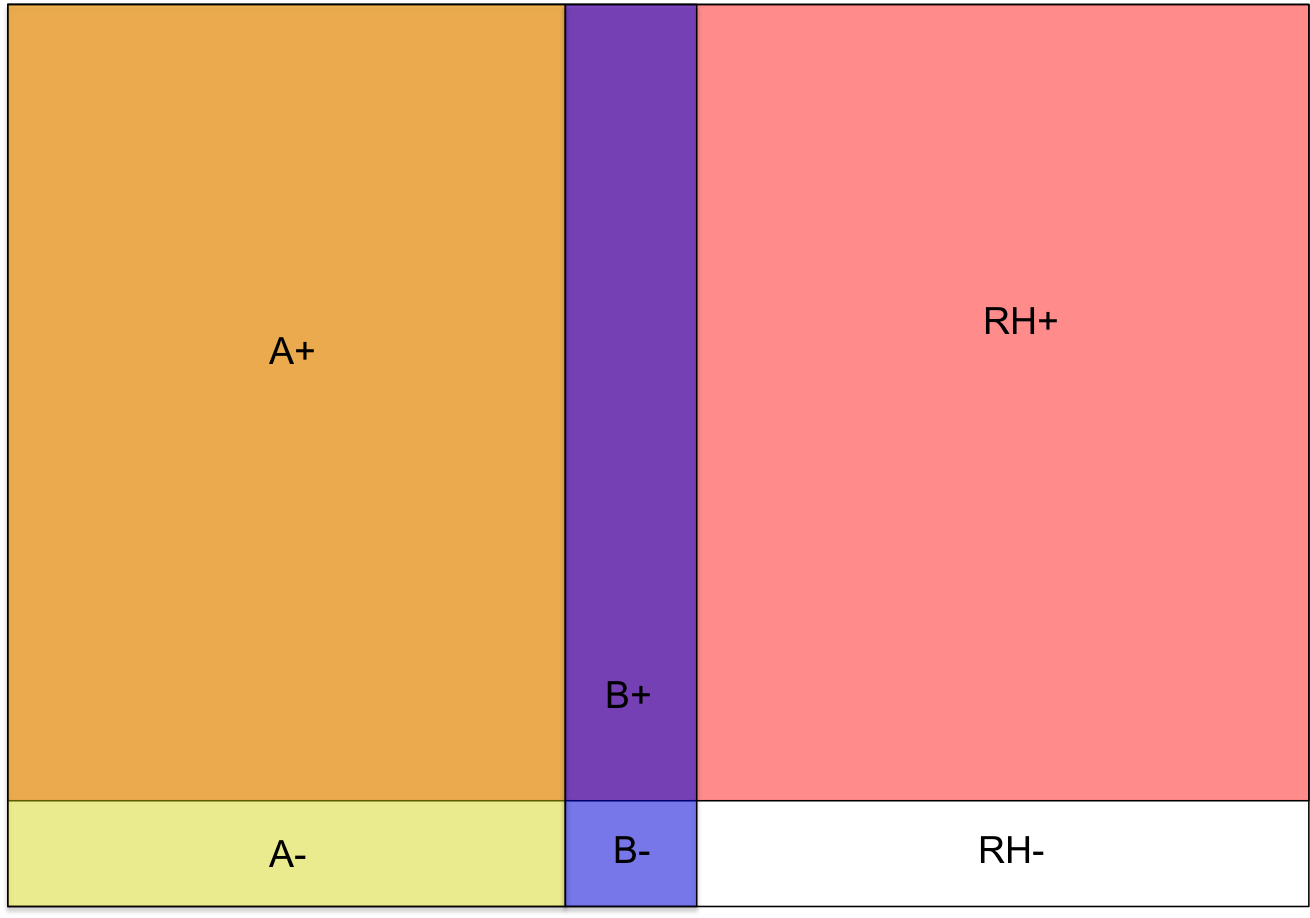
\includegraphics[width=.5\linewidth]{img/bloodvenndiag} 

}

\caption{Probabilities of blood types in humans. Areas are approximate.}\label{fig:bloodvendiag}
\end{figure}

Return to Figure \ref{fig:bloodvendiag} and consider two other events: a
person having blood type A or having the Rh factor (RH+). We see in
Figure \ref{fig:bloodvendiag} that someone can have both type A blood
and the Rh factor (blood type A+). Define:

\begin{itemize}
\tightlist
\item
  Event \(Y\) = a person has blood type A
\item
  Event \(Z\) = a person has the Rh factor
\item
  Event \(Y \cup Z\) = a person has blood type A or the Rh factor
\item
  Event \(Y \cap Z\) = a person has blood type A and the Rh factor (they
  have A+ blood)
\end{itemize}

So, the probabilty that someone has either type A blood or has the Rh
factor is the sum of probability of having type A blood (represented by
the yellow circle) and the probability of having the Rh factor
(represented by the red rectangle) minus the probability of having A+
blood (represented by the orange area of overlap that is counted twice)
in Figure \ref{fig:bloodvendiag}. So, the probability that a randomly
selected person has blood type A or the Rh factor is:

\[ P(Y \cup Z) = \_\_\_ \quad + \quad \_\_\_ \quad - \quad \_\_\_\]

\subsection{Conditional Probability}\label{conditional-probability}

Let's consider an event of interest \(Y\) which has probability
\(P(Y)\). Then, suppose we learn of another event of interest \(Z\) that
has occurred. Knowing that \(Z\) has occurred already may change our
opinion about the likelihood of \_\_\_\_\_ occurring. The key idea here
is that the probability of an event often depends on other information,
leading us to the definition of \emph{conditional probability}:

\[ P(Y|Z), \] which is the conditional \_\_\_\_\_\_\_\_\_\_\_\_\_\_ that
\(Y\) occurs given that we know \(Z\) has occurred. Return to Figure
\ref{fig:bloodvendiag}. Suppose we want to know the probability of a
person having type A blood, represented by the yellow circle. But, if we
already know that a person has the Rh factor, we are only interested in
the part of the type A circle that overlaps with the Rh+ rectangle. Thus
the probability of having type A blood is different with different
knowledge. The formula for calculating conditional probability is:

\begin{equation}\label{eq:2}
P(Y|Z) = \frac{P(Y\cap Z)}{P(Z)}
\end{equation}

Returning to the venn diagram, the value \(P(Y \cap Z)\) is represented
by the overlap of the type A circle and the Rh+ rectangle, and the value
\(P(Z)\) is represented by the Rh+ rectangle. Then, the value \(P(Y|Z)\)
is the ratio of the overlap (A+) to the Rh+ rectangle.

Equation \ref{eq:2} also gives us a multiplication rule for computing
probabilities:

\begin{equation}\label{eq:3}
P(Y\cap Z) = P(Y|Z) \cdot P(Z)
\end{equation}

Philosophically speaking, it can be helpful to think of \emph{all}
probabilities as conditional. It is just a question of what information
is assumed to be \_\_\_\_\_\_\_\_\_\_\_.

\subsubsection{Examples}\label{examples-1}

\textbf{Death Penalty Convictions}

A study of sentencing of 362 black people convicted of murder in Georgia
in the 1980s found that 59 were sentenced to death (Baldus, Pulaski, and
Woodworth (\protect\hyperlink{ref-baldus}{1983})). They also examined
the race of the murder victim, either black or white, and found some
disparities. In Table \ref{tab:dp}, DP means the defendant received the
death penalty, NDP means the defendant did not receive the death
penalty. The race of the victim (RV) is either black (B) or white (W).

\begin{table}
\centering
\begin{tabular}{l|cc|r}
RV & DP & NDP & Total \\
\hline
W & 45 & 85 & 130 \\
B & 14 & 218 & 232 \\
\hline
Total & 59 & 303 & 362
\end{tabular}
\caption{\label{tab:dp}The results of the Baldus et al study for black defendants convicted of murder.}
\end{table}

Returning to Section \ref{definitions}, let's define the problem:

\begin{itemize}
\tightlist
\item
  \textbf{Population}: All black people convicted of murder in Georgia
  in the 1980s
\item
  \textbf{Sample}: N/A (the whole population was studied)
\end{itemize}

Using the numbers from Table \ref{tab:dp}, compute the following
probabilities:

\begin{itemize}
\tightlist
\item
  \(P(DP) = \frac{\quad}{\quad} = 0.\_\_\_\) \vspace{.1in}
\item
  \(P(DP | RV = W) = \frac{\quad}{\quad} = 0.\_\_\_\) \vspace{.1in}
\item
  \(P(DP | RV = B) = \frac{\quad}{\quad} = 0.\_\_\_\) \vspace{.1in}
\end{itemize}

Note: These numbers are selected from the study, and should not be
considered a comprehensive summary of its results. There are a number of
things not discussed here. The entire publication can be found
online\footnote{\url{http://scholarlycommons.law.northwestern.edu/cgi/viewcontent.cgi?article=6378\&context=jclc}.}

\textbf{Consecutive Matching Striae}

In firearms and toolmark analysis, the number of consecutive matching
striae (CMS) between a crime scene sample and a lab sample is often used
to help determine a match. Generally speaking, the higher the maximum
number of CMS found in a pair, the more likely the two samples came from
the same source. Several known match (KM) pairs and known non-match
(KNM) pairs of bullets were examined, and the results are shown in
Figure \ref{fig:cms} (Hare, Hofmann, and Carriquiry
(\protect\hyperlink{ref-hare}{2017})). What is the probability of seeing
two known matches (or two known non-matches) given the maximum number of
CMS? Here, we condition on
\_\_\_\_\_\_\_\_\_\_\_\_\_\_\_\_\_\_\_\_\_\_\_\_\_\_. Again, we briefly
return to Section \ref{definitions}, let's define the problem:

\begin{itemize}
\tightlist
\item
  \textbf{Population}: All pairs of fired bullets from unknown sources
\item
  \textbf{Sample}: A sample of pairs of known matches and known
  non-matches
\end{itemize}

\begin{figure}[h]

{\centering 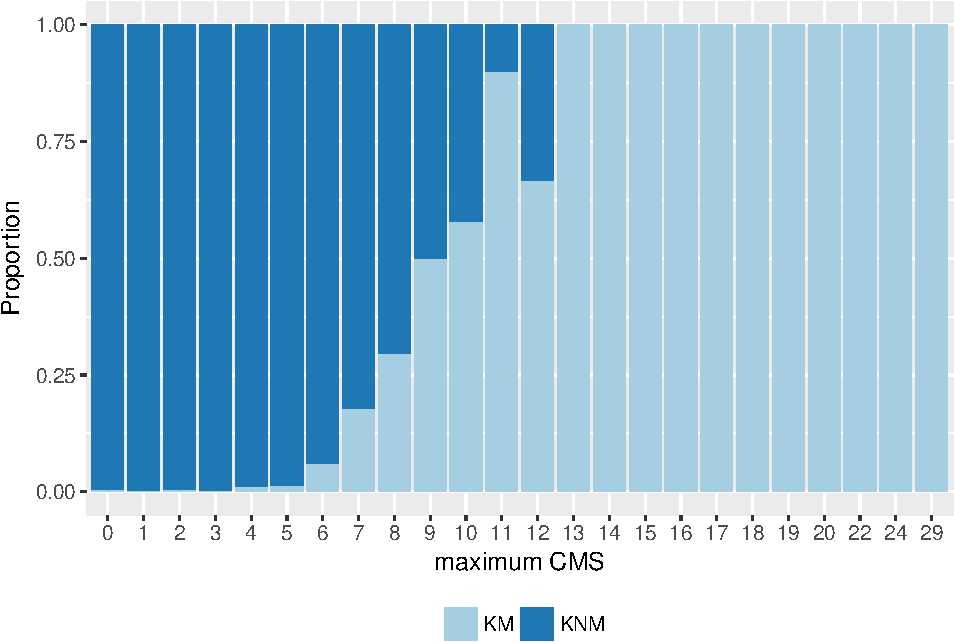
\includegraphics[width=.6\linewidth]{STfFP-Workbook_files/figure-latex/cms-1} 

}

\caption{This bar chart represents the conditional probabilities of two bullets matching given the maximum number of CMS. The light blue represents known matches, while the dark blue represents known non-matches.}\label{fig:cms}
\end{figure}

Generally, as seen in Figure \ref{fig:cms}, the probability of finding a
match tends to increase with then number of maximum CMS. For \_\_\_\_\_
maximum CMS values is it much more likely that we have a
\_\_\_\_\_\_\_\_\_\_\_\_\_\_\_\_\_\_ pair.

\subsection{Independence}\label{independence}

If the likelihood of one event is \emph{not} affected by knowing whether
a second has occured, then the two events are said to be
\_\_\_\_\_\_\_\_\_\_\_\_\_\_\_\_\_\_. For example, the region of the
country where you live and what color car you drive are (probably) not
related.

The death penalty example from the previous section demonstrates that
defendants receiving the death penalty is \emph{not} independent of the
race of the victim. In other words, a black defendant found guilty of
murder in Georgia in the 1980s received a different penalty depending on
the race of the victim.

Another example from DNA analysis relies on on independence across
chromosomes. By using loci on different chromosomes, there is
independence between the allele counts, allowing for simple calculation
of random match probabilities.

\subsection{Probability Math\ldots{}Again}\label{probability-mathagain}

Recall Equation \ref{eq:3}, which gives us the probability of two
events, \(Y\) and \(Z\) occurring together:

\[ P(Y \cap Z) = P(Z)\cdot P(Y|Z) = P(Y) \cdot P(Z|Y) \]

If \(Y\) and \(Z\) are \emph{independent}, there is a simple formula:

\[P(Y \cap Z) = \_\_\_\_ \cdot \_\_\_\_\]

This is because \(Z\) occurring does not effect the probability of \(Y\)
occurring, and vice versa. Thus,

\[ P(Y|Z) = P(Y) \quad \text{and} \quad P(Z|Y) = P(Z)\]

For example, the probability of being left-handed and from Florida is
equal to the probability of being left-handed times the probability of
being from Florida, assuming the events ``being left-handed'' and
``being from Florida'' are independent.

Multiplying probabilities of events directly like this is \emph{only}
applicable when the events are independent. When \emph{dependent} events
are treated as independent events, things can go terribly wrong. An
infamous example of this in the courts is the case
\textit{People v. Collins}\footnote{\emph{People v. Collins}, 68 Cal.2d
  319, 438 P.2d 33 (1968)}. This was a robbery trial, where eyewitnesses
described the robbers a ``black male with a beard and a moustache, and a
white female with a blonde ponytail, fleeing in a yellow car''.

The prosecution provided estimated probabilities of each of these
individual characteristic:

\begin{itemize}
\tightlist
\item
  P(black man with a beard) = \_\_\_\_\_\_\_\_\_\_\_\_
\item
  P(black man with a moustache) = \_\_\_\_\_\_\_\_\_\_\_\_
\item
  P(white woman with ponytail) = \_\_\_\_\_\_\_\_\_\_\_\_
\item
  P(white woman with blonde hair) = \_\_\_\_\_\_\_\_\_\_\_\_
\item
  P(yellow car) = \_\_\_\_\_\_\_\_\_\_\_\_
\item
  P(interratial couple in a car) = \_\_\_\_\_\_\_\_\_\_\_\_
\end{itemize}

A mathematics ``expert'' talked about the so-called ``multiplication
rule for probability'', and directly multiplied the above probabilities
together without considering that the events could be \emph{dependent}.
i.e.~a man with a beard probably has a much higher chance of having a
moustache than a man with no beard. Due to this faulty math, the
conviction was set aside and the statistical reasoning criticized for
ignoring dependence among the characteristics.

In a courtroom situation, let \(S\) be the event that the suspect was
present at the scene of the crime and \(\overline{S}\) be the event that
the suspect was not present at the scene. Assume that each juror has in
mind an initial probability for the events \(S\) and \(\overline{S}\).
Then, a witness says they saw a tall Caucasian male running from the
scene, and the defendant is a tall Caucasian male. After hearing the
witness' testimony, the jurors \_\_\_\_\_\_\_\_\_ their probabilities.
Next, an expert witness testifies that fragments from a window broken
during the crime and fragments found on the defendant's clothing match.
Again, the jurors update their \_\_\_\_\_\_\_\_\_\_\_\_. This process
continues throughout the trial. There are some key questions to
consider:

\begin{itemize}
\tightlist
\item
  How should jurors update their probabilities?
\item
  Do jurors \emph{actually} think this way?
\end{itemize}

\subsection{Bayes' Rule}\label{bayes-rule}

\emph{Bayes' Rule} provides an \_\_\_\_\_\_\_\_\_ formula for
probabilities. Like in the trial scenario above, suppose we have an
initial estimate for the probability of event \(S\), \(P(S)\). Then, we
learn that an event \(R\) has occurred and we want to update or
probability of event \(S\). To do this, we need to know about the
\_\_\_\_\_\_\_\_\_\_\_\_ of \(R\) and \(S\). To update the probability
of \(S\), we can use Bayes' Rule, also called Bayes'
\_\_\_\_\_\_\_\_\_\_\_:

\begin{equation}\label{eq:4}
\begin{split}
P(S|R) & = \frac{P(R \cap S)}{P(R)} = \frac{P(R|S)P(S)}{P(R)} \\
& = \frac{P(R|S)P(S)}{P(R|S)P(S) + P(R|\overline{S})P(\overline{S})} 
\end{split}
\end{equation}

\begin{figure}

{\centering 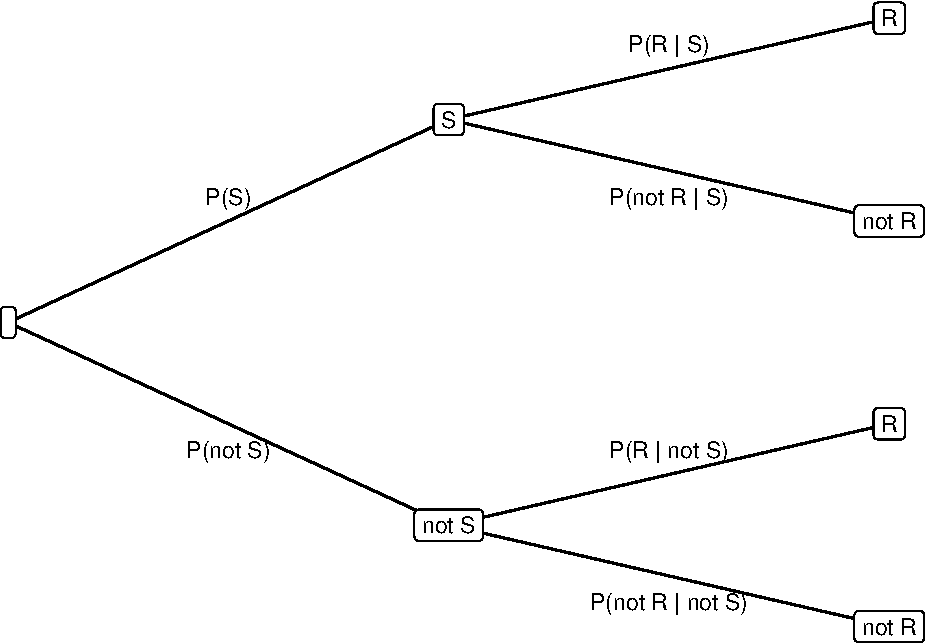
\includegraphics[width=.7\linewidth]{STfFP-Workbook_files/figure-latex/probtree-1} 

}

\caption{A probability tree showing the direction of flow when updating probabilities. Move from left to right on the tree through the events possible. Events are in boxes, probabilities are on the branches of the tree.}\label{fig:probtree}
\end{figure}

\subsubsection{Examples}\label{examples-2}

Consider performing diagnostic tests for gunshot residue.

\begin{itemize}
\tightlist
\item
  Let \(G\) denote the presence of gunshot residue \vspace{.1in}
\item
  Let \(\overline{G}\) denote the \_\_\_\_\_\_\_\_\_\_\_\_ of gunshot
  residue \vspace{.1in}
\item
  Let \(T\) denote a \_\_\_\_\_\_\_\_\_\_\_\_\_ diagnostic test
  \vspace{.1in}
\item
  Let \(\overline{T}\) denote a negative diagnostic test
\end{itemize}

\begin{table}[h]
\centering
\begin{tabular}{|l|c|c|}
\hline
Truth & $T$ & $\overline{T}$ \\
\hline
$G$ & True Positive & False Negative \\
\hline
$\overline{G}$ & False Positive & True Negative \\
\hline
\end{tabular}
\caption{\label{tab:bayesex} All potential outcomes of a diagnostic test for gunshot residue.}
\end{table}

The values in the table can also be thought of as conditional
probabilities:

\begin{itemize}
\tightlist
\item
  The value \(P(T|G)\) is the
  \_\_\_\_\_\_\_\_\_\_\_\_\_\_\_\_\_\_\_\_\_\_\_ rate, also called
  \emph{sensitivity} of the test \vspace{.1in}
\item
  The value \(P(\overline{T}|\overline{G})\) is the
  \_\_\_\_\_\_\_\_\_\_\_\_\_\_\_\_\_\_\_\_ rate, also called the
  \emph{specificity} of the test \vspace{.1in}
\item
  The value \(P(T|\overline{G})\) is the
  \_\_\_\_\_\_\_\_\_\_\_\_\_\_\_\_\_\_\_\_\_\_ rate, the Type I error
  rate \vspace{.1in}
\item
  The value \(P(\overline{T}|G)\) is the
  \_\_\_\_\_\_\_\_\_\_\_\_\_\_\_\_\_\_\_\_\_\_\_\_ rate, the Type II
  error rate
\end{itemize}

Studies of the diagnostics test usually tell us \(P(T|G)\),
\_\_\_\_\_\_\_\_\_\_\_, and \(P(\overline{T}|\overline{G})\),
\_\_\_\_\_\_\_\_\_\_ . Examiners may begin with some idea of \(P(G)\),
or the \_\_\_\_\_\_\_\_\_\_\_ of gunshot residue in a similar situation.
What is most relevent for the case is the \emph{postitive predictive
value}, or in probability notation, \_\_\_\_\_\_\_\_\_\_\_. We can use
\_\_\_\_\_\_\_\_\_\_\_\_\_\_\_\_\_\_\_\_\_\_\_\_\_\_ to obtain this
value:

\[ P(G|T) = \frac{P(T|G)P(G)}{P(T|G)P(G) + P(T|\overline{G})P(\overline{G})}\]

Generally speaking, the most important thing to remember is that, in
general, \(P(T|G) \quad \_\_\_\_ \quad P(G|T)\).

The careful application of Bayes' Rule can sometimes lead to surprising,
non-intuitive results. Continuing with the gunshot residue test example,
assume

\begin{itemize}
\tightlist
\item
  sensitivity is 98\% (\(P(\quad|\quad) = 0.98\)) \vspace{.1in}
\item
  specificity is 96\% (\(P(\quad|\quad) = 0.96\)) \vspace{.1in}
\item
  prevalence is 90\% (\(P(\quad) = 0.90\)) \vspace{.1in}
\item
  Plug values into the Bayes' Rule formula to find \(P(G|T)\):

  \begin{equation}\label{eq:5}
  \begin{split}
   P(G|T) & = \frac{P(T|G)P(G)}{P(T|G)P(G) + P(T|\overline{G})P(\overline{G})} \\ 
   & = \frac{0.98 \cdot 0.9}{0.98 \cdot 0.9 + (1- 0.96)\cdot (1-0.9)} \\ 
   & = \frac{0.882}{0.882 + 0.004} \\
   & = 0.995
  \end{split}
  \end{equation}
\item
  Now assume prevalence is 10\% (\(P(\quad) = 0.10\)) and plug in the
  values again \vspace{.1in}

  \begin{equation}\label{eq:6}
  \begin{split}
   P(G|T) & = \frac{P(T|G)P(G)}{P(T|G)P(G) + P(T|\overline{G})P(\overline{G})} \\ 
   & = \frac{0.98 \cdot 0.1}{0.98 \cdot 0.1 + (1- 0.96)\cdot (1-0.1)} \\ 
   & = \frac{0.098}{0.098 + 0.036} \\
   & = \frac{0.098}{0.134} \\
   & = 0.731
  \end{split}
  \end{equation}
\item
  So, even if there is a postive test, we are not really sure about
  whether gunshot residue is \emph{actually} present.
\item
  Why does this happen?? See Figure \ref{fig:probtree2}.
\end{itemize}

\begin{figure}[h]

{\centering 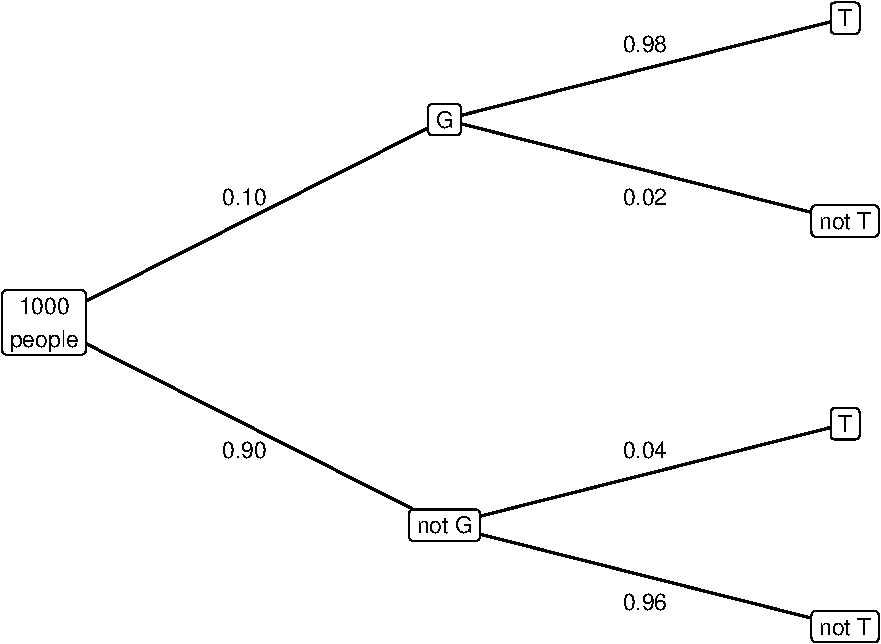
\includegraphics[width=.7\linewidth]{STfFP-Workbook_files/figure-latex/probtree2-1} 

}

\caption{A probability tree showing the direction of flow when updating probabilities for the presence of gunshot residue. Suppose there are 1,000 people in the population you're considering. Write the number of people in the groups throughout the tree according to the probabilities indicated on the branches of the tree}\label{fig:probtree2}
\end{figure}

\subsection{Bayes' Rule to the Likelihood
Ratio}\label{bayes-rule-to-the-likelihood-ratio}

In the general forensic setting, let \(S\) denote the event that the
evidence from the scene and comparison sample are from the same source.
Let \(E\) denote the evidence found at the scene. The formulation of
Bayes' Rule for this situation is:

\[ P(S|E) = \frac{P(E|S)P(S)}{P(E|S)P(S) + P(E|\overline{S})P(\overline{S})}\]

We can rewrite Bayes' Rule in terms of odds:

\begin{equation}\label{eq:odds}
\frac{P(S|E)}{P(\overline{S}|E)} = \frac{P(E|S)}{P(E|\overline{S})}\frac{P(S)}{P(\overline{S})}
\end{equation}

Derivation of Equation \ref{eq:odds} is shown in Equation \ref{eq:7}.
For now, just consider Equation \ref{eq:odds}:

\begin{itemize}
\tightlist
\item
  On the left, \(\frac{P(S|E)}{P(\overline{S}|E)}\) are the odds in
  favor of \(S\) given the evidence \(E\).
\item
  The last term on the right, \(\frac{P(S)}{P(\overline{S})}\) are the
  odds in favor of \(S\) before seeing the evidence \(E\) (the ``prior
  odds'') \vspace{.1in}
\item
  The first term on the right \(\frac{P(E|S)}{P(E|\overline{S})}\), is
  known as the \_\_\_\_\_\_\_\_\_\_\_\_\_ ratio \vspace{.1in}
\item
  The likelihood ratio (LR) is the factor by which we
  \_\_\_\_\_\_\_\_\_\_\_ prior odds of two samples being from the same
  source to get \_\_\_\_\_\_\_\_\_\_\_\_\_\_ odds (after seeing
  evidence) of the same source.
\end{itemize}

\begin{equation}\label{eq:7}
\begin{split}
P(S|E) & = \frac{P(E|S)P(S)}{P(E|S)P(S) + P(E|\overline{S})P(\overline{S})} \\
\Rightarrow \frac{1}{P(S|E)} & = \frac{P(E|S)P(S) + P(E|\overline{S})P(\overline{S})}{P(E|S)P(S)} \\ 
  & = 1 + \frac{P(E|\overline{S})P(\overline{S})}{P(E|S)P(S)} \\ 
\Rightarrow \frac{1}{P(S|E)} -1 & = \frac{P(E|\overline{S})P(\overline{S})}{P(E|S)P(S)} \\ 
\frac{1}{P(S|E)} - \frac{P(S|E)}{P(S|E)} & = \\
\frac{1-P(S|E)}{P(S|E)} & = \\
\frac{P(\overline{S}|E)}{P(S|E)} & =  \frac{P(E|\overline{S})P(\overline{S})}{P(E|S)P(S)} \\
\Rightarrow \frac{P(S|E)}{P(\overline{S}|E)} & = \frac{P(E|S)P(S)}{P(E|\overline{S})P(\overline{S})} 
\end{split}
\end{equation}

\subsubsection{Examples}\label{examples-3}

Return to the gunshot residue (GSR) test example. Define:

\begin{itemize}
\tightlist
\item
  \(E\) = evidence = a positive test for (GSR)
\item
  \(S\) = suspect has GSR on them
\end{itemize}

\[LR = \frac{P(E|S)}{P(E|\overline{S})} = \frac{0.98}{0.04} = 24.5\]

In a high prevalence case (\(P(G)=0.9\)), the prior odds are
\(\frac{0.9}{0.1} = 9\). The posterior odds are \(LR \times\)prior odds
\(= 24.5\times 9 = 220.5:1\).

In a low prevalence case (\(P(G)=0.1\)), the prior odds are
\(\frac{0.1}{0.9} = \frac{1}{9}\). The posterior odds are
\(LR \times\)prior odds \(= 24.5\times \frac{1}{9} = 24.5:9 = 2.72:1\).

We can also compute the likelihood ratio if the evidence were a negative
test. This value turns out to be \(\frac{1}{48}\), which is \textbf{not}
the reciprocal of the LR for the positive test.

\subsection{Recap}\label{recap}

\begin{itemize}
\tightlist
\item
  Probability is the \_\_\_\_\_\_\_\_\_\_\_\_\_ language of
  \_\_\_\_\_\_\_\_\_\_\_\_\_ \vspace{.1in}
\item
  Provides a common scale, from \_\_\_\_\_ to \_\_\_\_\_, for describing
  the chance that an event will occur \vspace{.1in}
\item
  \textbf{Conditional} probability is a key concept! The probabilitity
  of an event depends on what \_\_\_\_\_\_\_\_\_\_\_\_ is available
  \vspace{.1in}
\item
  Independent events can be powerful! They allow us to
  \_\_\_\_\_\_\_\_\_ probabilities of events \emph{directly}, as is
  common in \_\_\_\_\_\_\_\_\_\_\_\_\_\_\_\_\_. \vspace{.1in}
\item
  \_\_\_\_\_\_\_\_\_\_\_\_\_\_\_\_\_\_\_\_ is a mathematical result
  showing how we should \_\_\_\_\_\_\_\_\_\_\_ our probabilities when
  available information changes. \vspace{.1in}

  \begin{itemize}
  \tightlist
  \item
    This will later lead us to the likelihood ratio as a numerical
    \_\_\_\_\_\_\_\_\_\_\_\_ of the evidence. \vspace{.1in}
  \item
    Bayes' Rule does not necessarily describe how people operate in
    practice.
  \end{itemize}
\end{itemize}

\subsection{Probability and the
Courts}\label{probability-and-the-courts}

Sally Clark was the only person in the house when her first child died
unexpectedly at 3 months old. The cause of death was determined to be
SIDS, sudden infant death syndrome. One year later, Sally and her
husband had a second child, who died at 2 months old under similar
circumstances. Sally was convicted of murder.

During her trial, a pediatrician testified that the probability of a
single SIDS death for a family like the Clarks (similar income, etc.)
was \(\frac{1}{8500}\approx 0.0001\), and thus the probability of two
SIDS death in the family was
\(\frac{1}{8500^2} = \frac{1}{73 \times 10^6} \approx 1.37 \times 10^{-8}\).
There are several problems with this approach to evidence. What do you
think? Jot down a few ideas below: \vspace{.1in}

\rule{\textwidth}{.4pt}

\vspace{.1in}

\rule{\textwidth}{.4pt}

\vspace{.1in}

\rule{\textwidth}{.4pt}

\vspace{.1in}

Issues with the evidence presented by the pediatrician:

\begin{enumerate}
\def\labelenumi{\arabic{enumi}.}
\tightlist
\item
  Is the probability of a child dying of SIDS given, \(\frac{1}{8500}\),
  correct for ``families like the Clarks''?
\item
  The use of direct multiplication of probabilities assumes independence
  of the two deaths in the family. (Independence within the family is
  not a reasonable assumption.)
\item
  Alternative hypotheses (causes of death of the infants) were not
  considered. Did something else with perhaps a higher likelihood cause
  the children's deaths?
\end{enumerate}

\section{Probability to Statistical
Inference}\label{probability-to-statistical-inference}

Probability is important, but it is only one tool in our toolbox.
Another, more powerful tool is statistical inference.

\subsection{Collecting Data}\label{collecting-data}

First, we consider data collection. Where do data come from? One data
source is an \emph{experiment}. An investigator designs a study and
collects information on and maybe applies treatments to a \emph{sample},
a subset of the population of interest. \_\_\_\_\_\_\_\_\_ can tell us a
great deal about how to design an \_\_\_\_\_\_\_\_\_\_\_ or choose a
\_\_\_\_\_\_\_\_\_.

The area of statistics concerned with creating studies is called
\emph{experimental design}. The experimental design literature is
extensive (see for example Morris (\protect\hyperlink{ref-doe}{2011})).
Here are a few crucial points:

\begin{itemize}
\tightlist
\item
  The goal of an experiment is to compare \_\_\_\_\_\_\_\_\_\_\_\_
  \vspace{.1in}
\item
  Those \_\_\_\_\_\_\_\_\_\_\_\_ must be \_\_\_\_\_\_\_\_\_\_\_ assigned
  to units \vspace{.1in}
\item
  The \_\_\_\_\_\_\_\_\_\_\_\_\_\_ in the experiment must be large
  enough t obe able to make informed conclusions
\item
  Blinding plays an important role in avoiding \_\_\_\_\_\_\_. e.g.
  ``double-blind'' studies in medicine, where neither the patient nor
  the doctor administering the treatment know which treatment the
  patient is receiving
\end{itemize}

How is experimental design relevant to forensic science?

\begin{itemize}
\tightlist
\item
  Experiments are used to evaluate process improvements
\item
  Blinding is used in ``black box'' studies, where examiners do not know
  ground truth
\end{itemize}

Experiments almost always involve \emph{sampling} from the population of
interest. Why?

\begin{itemize}
\tightlist
\item
  We sample because it is too \_\_\_\_\_\_\_\_\_ or
  \_\_\_\_\_\_\_\_\_\_\_\_\_ to study the \emph{entire} population
  \vspace{.1in}
\item
  A \_\_\_\_\_\_\_\_\_ sample allows us to use the laws of
  \_\_\_\_\_\_\_\_\_\_\_ to describe how certain we are that our
  \_\_\_\_\_\_\_\_\_\_\_\_ answer reflects the \_\_\_\_\_\_\_\_\_\_\_\_.
\item
  There are many famous failures (cautionary tales) with
  \_\_\_\_\_\_\_\_\_\_\_\_\_\_\_\_\_\_ sampling. (See Figure
  \ref{fig:dewey}.)
\end{itemize}

How is sampling relevant to forensic science?

\begin{itemize}
\tightlist
\item
  Sampling techniques used to determine which and how many bags of
  suspect powder collected from a crime scene to test.
\end{itemize}

\begin{figure}[h]

{\centering 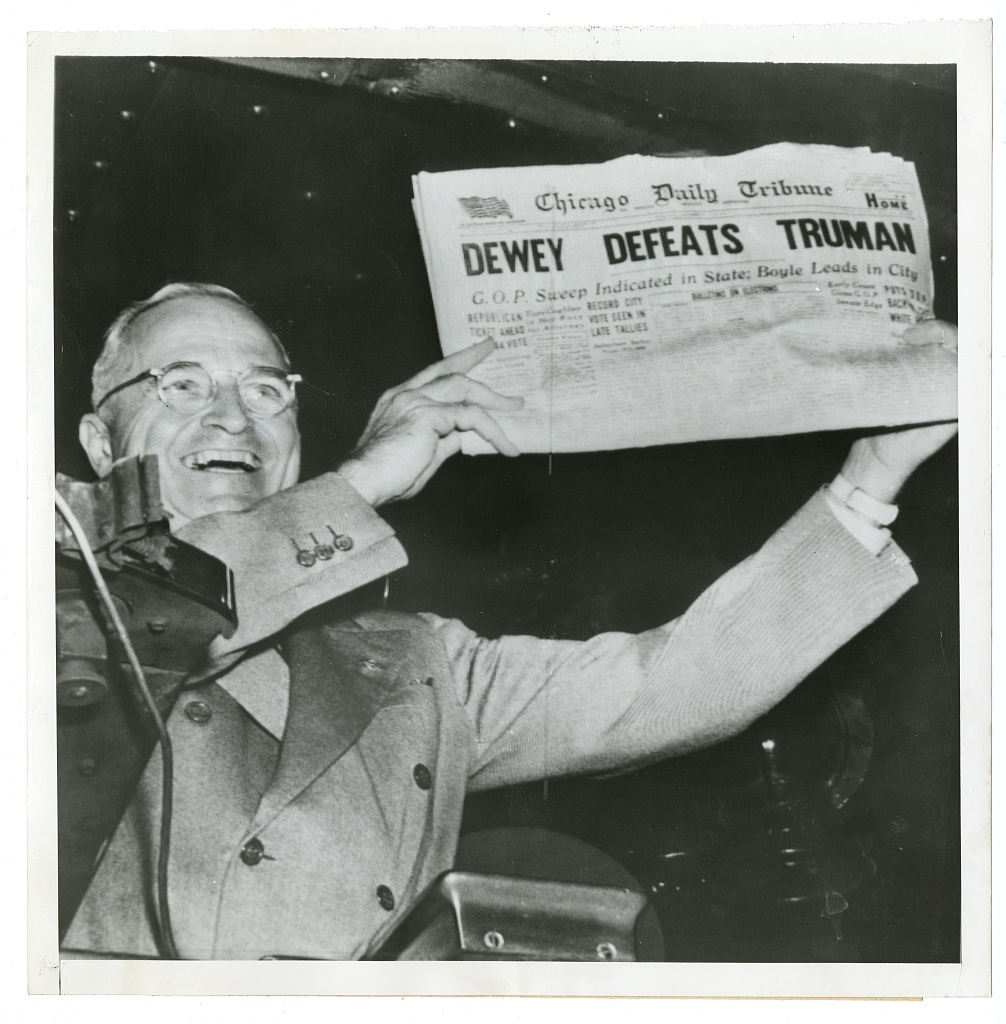
\includegraphics[width=.5\linewidth]{img/dewey} 

}

\caption{This picture from the US presidential election of 1948 shows President Harry Truman, who won the election, holding a newspaper that went to print with the headline "Dewey Defeats Truman!" The headline was based on biased sampling that favored typically Republican demographics. Image Source: https://blogs.loc.gov/loc/2012/11/stop-the-presses/}\label{fig:dewey}
\end{figure}

All data collected can be divided into one of two groups: qualitative or
quantitative.

\begin{itemize}
\tightlist
\item
  \textbf{Qualitative} data describe qualities about the observations.
  For example, the race of a suspect, or their level of education. There
  are two subcategories of qualitative data: \vspace{.1in}

  \begin{itemize}
  \tightlist
  \item
    \_\_\_\_\_\_\_\_\_\_\_\_\_\_: the data belong to one of a discrete
    number of groups or categories. For example: blood type (A, B, AB,
    or O) \vspace{.1in}
  \item
    \_\_\_\_\_\_\_\_\_\_\_\_\_\_: the data belong to one group in a set
    of ordered values. For example, the evaluation of a teacher (poor,
    average, excellent). The categories have an inherent ordering,
    unlike in categorical data.\vspace{.1in}
  \end{itemize}
\item
  \textbf{Quantitative} data describe quantities that can be measured on
  the observations. These are numerical data. There are also two
  subcategories of quantitative data: \vspace{.1in}

  \begin{itemize}
  \tightlist
  \item
    \_\_\_\_\_\_\_\_\_\_\_\_\_\_\_: the values are distinct or separate.
    An easy-to-understand example is integer observations:
    \(\{0,1,2,3,4, \dots \}\). A forensic science example is consecutive
    matching striae on bullets or toolmarks. (See Figure \ref{fig:cms})
  \item
    \_\_\_\_\_\_\_\_\_\_\_\_\_\_\_\_: the values can take on any value
    in a finite or infinite interval. Continuous values fall anywhere on
    the number line. A forensic science example is the refractive index
    of a glass fragment.
  \end{itemize}
\end{itemize}

\subsection{Probability Distributions}\label{probability-distributions}

Suppose we are to collect data on some characteristic for a sample of
individuals or objects (e.g.~weight, trace element concentration). A
probability \_\_\_\_\_\_\_\_\_\_\_ is used to describe these possible
values and how \_\_\_\_\_\_\_\_\_\_\_ each value is to occur. There are
many, many possible probability distributions, but some of the most
common are the Binomial, Poisson, Normal, and Lognormal distributions.
The probabilities associated with each of these distributions and their
possible outcomes are plotted in Figures
\ref{fig:binompois}-\ref{fig:normlnorm}.

\begin{itemize}
\tightlist
\item
  Discrete distributions \vspace{.1in}

  \begin{itemize}
  \tightlist
  \item
    \_\_\_\_\_\_\_\_\_\_\_\_\_\_\_\_\_: counts the number of
    \_\_\_\_\_\_\_\_\_\_ in a fixed number (\(n\)) of
    \_\_\_\_\_\_\_\_\_\_\_. Possible values are \(\{0,1,2, \dots, n\}\).
    \vspace{.1in}
  \item
    \_\_\_\_\_\_\_\_\_\_\_\_\_\_: counts the number of
    \_\_\_\_\_\_\_\_\_\_ occurring. Possible values are
    \(\{0,1,2,3,4,5,\dots\}\)
  \end{itemize}
\end{itemize}

\begin{figure}[h]

{\centering 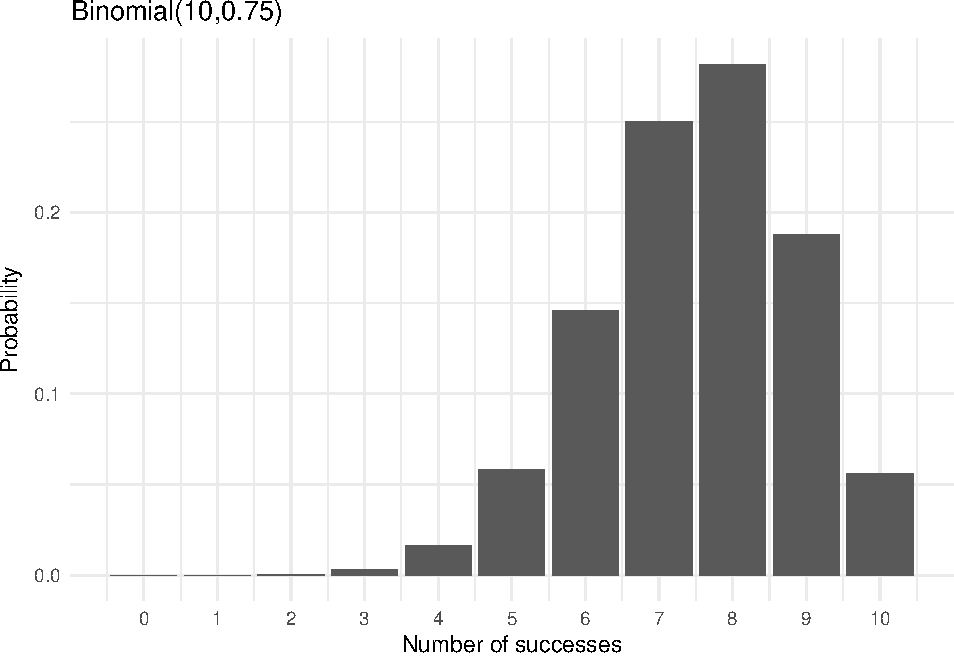
\includegraphics[width=.49\linewidth]{STfFP-Workbook_files/figure-latex/binompois-1} 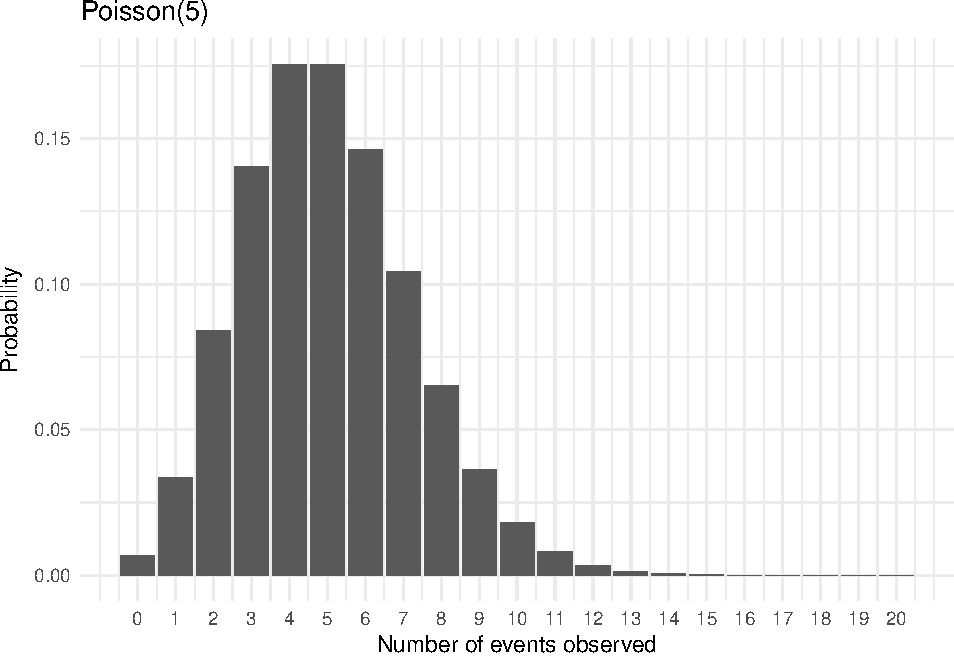
\includegraphics[width=.49\linewidth]{STfFP-Workbook_files/figure-latex/binompois-2} 

}

\caption{On the left, the probability of each possible outcome for variable with binomial distribution with 10 trials and probability of success 0.75. On the right, the probability of each possible outcome for variable with Poisson distribution with mean value 5.}\label{fig:binompois}
\end{figure}

\begin{itemize}
\tightlist
\item
  Continuous distributions \vspace{.1in}

  \begin{itemize}
  \tightlist
  \item
    \_\_\_\_\_\_\_\_\_\_\_\_\_\_\_: the famous, symmetric
    ``bell-shaped'' \_\_\_\_\_\_\_\_\_. Possible values are all real
    numbers, \((-\infty, \infty)\)
  \item
    \_\_\_\_\_\_\_\_\_\_\_\_\_\_: the (natural) logarithm of
    observations from this distribution follow a \_\_\_\_\_\_\_\_\_\_
    distribution. Possible values are all positive real numbers,
    \((0,\infty)\)
  \end{itemize}
\end{itemize}

\begin{figure}[h]

{\centering 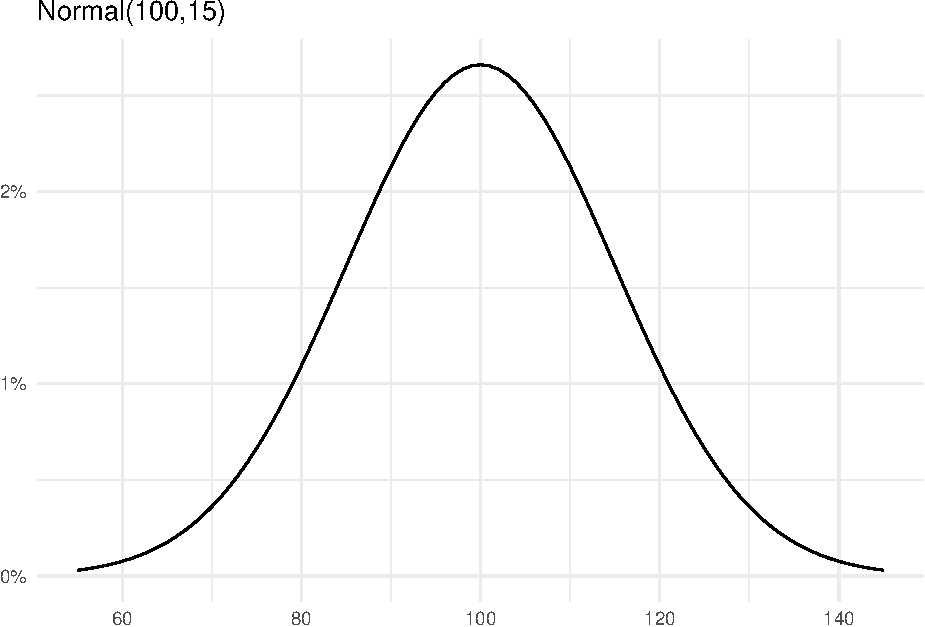
\includegraphics[width=.49\linewidth]{STfFP-Workbook_files/figure-latex/normlnorm-1} 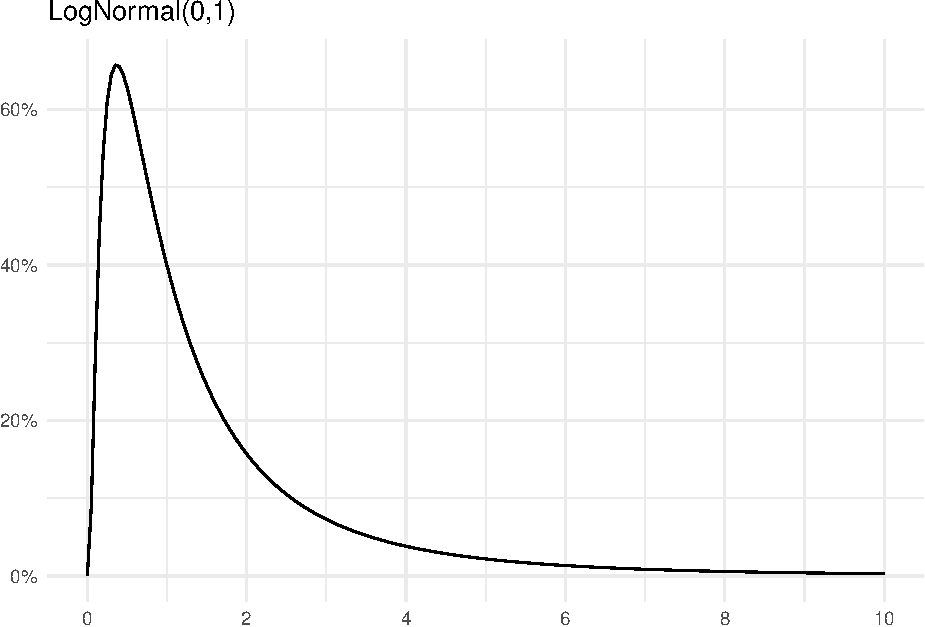
\includegraphics[width=.49\linewidth]{STfFP-Workbook_files/figure-latex/normlnorm-2} 

}

\caption{On the left, the probability distribution curve of possible outcomes for a variable with Normal distribution with mean value 100 and standard deviation 15. On the right, the probability distribution curve of possible outcomes for a variable with Lognormal distribution with mean value 0 and standard deviation 1.}\label{fig:normlnorm}
\end{figure}

\subsubsection{Normal}\label{normal}

You may already be familiar with this distribution with the bell-shaped
curve. Measurement error is one example of something often assumed to
follow a normal distribution. The normal distribution is described by
two parameters: the \_\_\_\_\_\_\_\_, denoted by \(\mu\), and the
\_\_\_\_\_\_\_\_\_\_\_\_\_\_\_\_\_\_\_\_, denoted by \(\sigma\). If we
have a variable (say, something observed in our data like weight), we
give the variable a capital letter, typically \(X\). If this variable
\(X\) is normally distributed with mean \(\mu\) and standard deviation
\(\sigma\), we write this as:

\[ X \sim N(\_\_\_, \_\_\_) \]

In measurement error, for example, we typically assume that the mean is
0. So, if \(X\) represents measurement error, we'd write
\(X \sim N(0,\sigma)\).

There are many nice properties of the normal distribution. For instance,
we know that \_\_\_\_\_\% of observable values lie within \_\_\_\_\_
standard deviations of the mean (\(\mu \pm 2\sigma\)), and also that
\_\_\_\_\_\% of observable values lie within \_\_\_\_\_ standard
deviations of the mean (\(\mu \pm 3\sigma\)). When working with the
normal distribution, we use software (such as Excel, Matlab, R, SAS,
etc.), tables\footnote{See for example
  \url{http://www.stat.ufl.edu/~athienit/Tables/Ztable.pdf}}, or
websites like
\href{http://onlinestatbook.com/2/calculators/normal_dist.html}{onlinestatbook.com}
or
\href{http://stattrek.com/online-calculator/normal.aspx}{stattrek.com}
to compute probabilities of events.

\begin{figure}[h]

{\centering 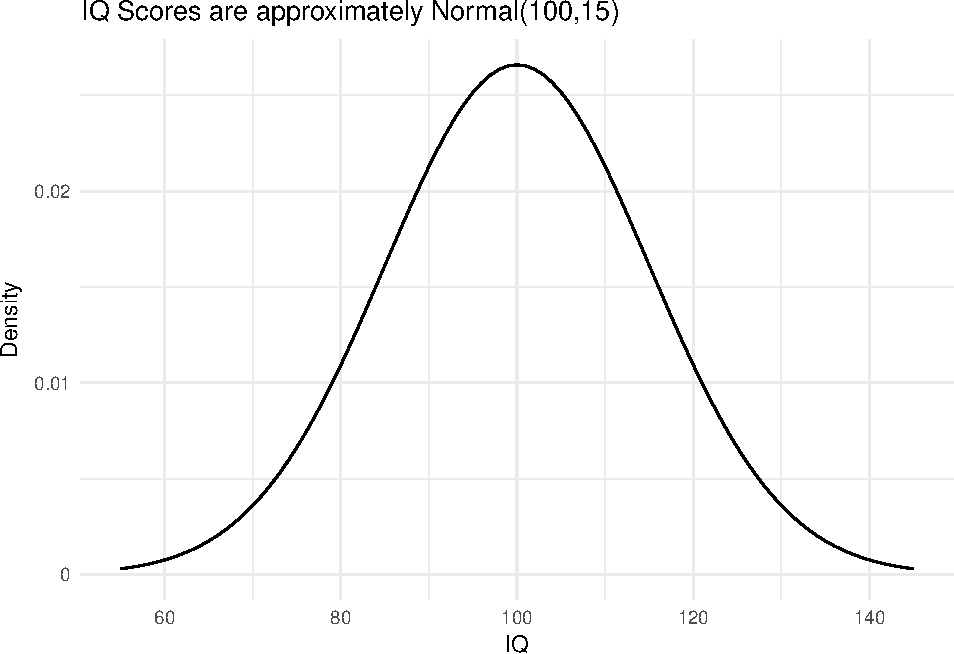
\includegraphics[width=.49\linewidth]{STfFP-Workbook_files/figure-latex/norm4-1} 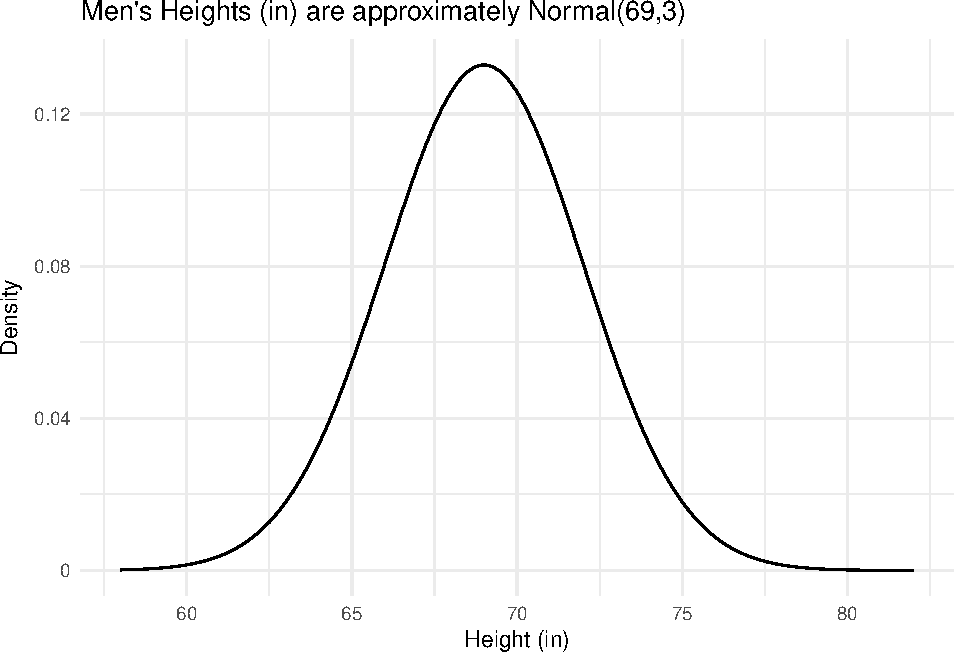
\includegraphics[width=.49\linewidth]{STfFP-Workbook_files/figure-latex/norm4-2} 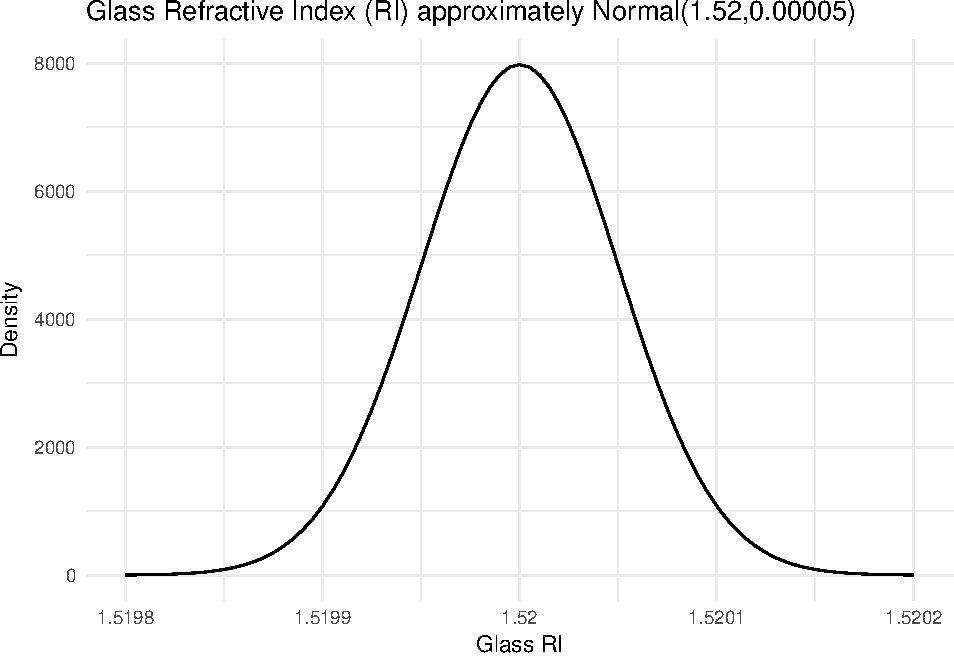
\includegraphics[width=.49\linewidth]{STfFP-Workbook_files/figure-latex/norm4-3} 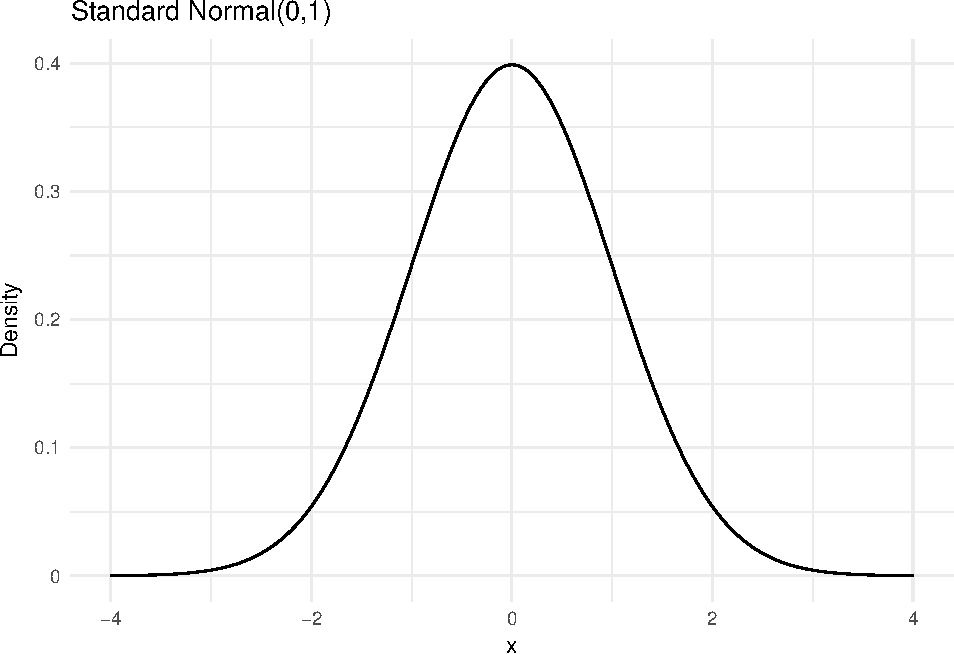
\includegraphics[width=.49\linewidth]{STfFP-Workbook_files/figure-latex/norm4-4} 

}

\caption{Four examples of the probability distribution functions for normally distributed variables}\label{fig:norm4}
\end{figure}

\subsubsection{Lognormal}\label{lognormal}

We often act as if everything is normally distributed, but of course
this is not true. For instance, a quantity that is certain to be
\_\_\_\_\_\_\_\_\_\_\_ (greater than or equal to zero) cannot possible
be normally distributed. Consider trace element concetration: either
none is detected, or there is some amount greater than 0 detected.

In cases where nonnegative values are not possible, we may believe that
the (natural) \_\_\_\_\_\_\_\_\_ of the quantity is normal, which gives
us a \_\_\_\_\_\_\_\_\_\_ distribution for the quantity itself. The
lognormal distribution, like the normal, has two parameters: mean (on
the log scale), denoted \_\_\_\_\_, and standard deviation (on the log
scale), denoted \_\_\_\_\_.

\begin{figure}[h]

{\centering 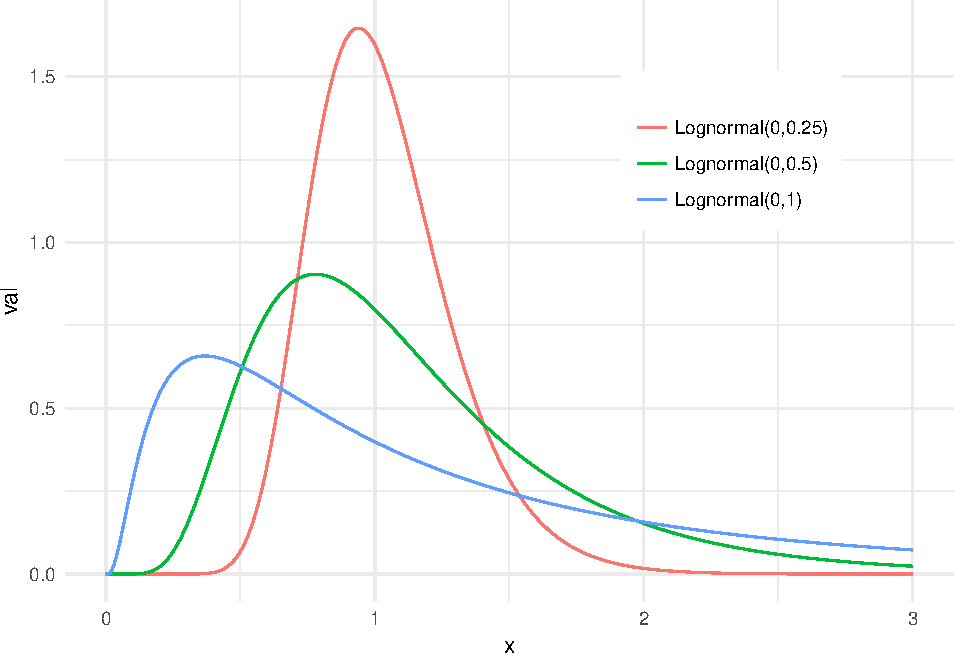
\includegraphics[width=.5\linewidth]{STfFP-Workbook_files/figure-latex/lognorm-1} 

}

\caption{Three lognormal distributions with the same mean (on the log scale) and different standard deviations (on the log scale)}\label{fig:lognorm}
\end{figure}

\subsubsection{Discrete}\label{discrete}

Some quantities take on very few possible values. These are
\emph{discrete} data.

Recall the two common discrete distributions from section
\ref{probability-distributions}:

\begin{itemize}
\tightlist
\item
  Binomial: \vspace{.1in}

  \begin{itemize}
  \tightlist
  \item
    Data are \_\_\_\_\_\_\_\_ (two categories: ``success'' or
    ``failure'') \vspace{.1in}
  \item
    Data are a result of \(n\) independent \_\_\_\_\_\_\_\_\_
    \vspace{.1in}
  \item
    \(P(\text{success}) = p\) on each trial. (Same \_\_\_\_\_\_\_\_\_ of
    success each time) \vspace{.1in}
  \item
    Expected number of successes you expect to see out of \(n\) trials:
    \_\_\_\_\_ \(\times\) \_\_\_\_\_ \vspace{.1in}
  \item
    Example: Suspect a student of cheating on an exam, response is the
    number of correct answers.
  \end{itemize}
\item
  Poisson: \vspace{.1in}

  \begin{itemize}
  \tightlist
  \item
    Data are counts: number of events occurring in a \_\_\_\_\_\_\_\_\_
    time \vspace{.1in}
  \item
    The mean and the \_\_\_\_\_\_\_\_\_\_\_\_ of this distribution are
    the same, so the variablility in responses increases as the
    \_\_\_\_\_\_\_\_\_ increases. \vspace{.1in}
  \item
    Example: number of calls to 911 between 10:00 and midnight on Friday
    nights. See Figure \ref{fig:cmspois} for a forensics example.
  \end{itemize}
\end{itemize}

\begin{figure}[h]

{\centering 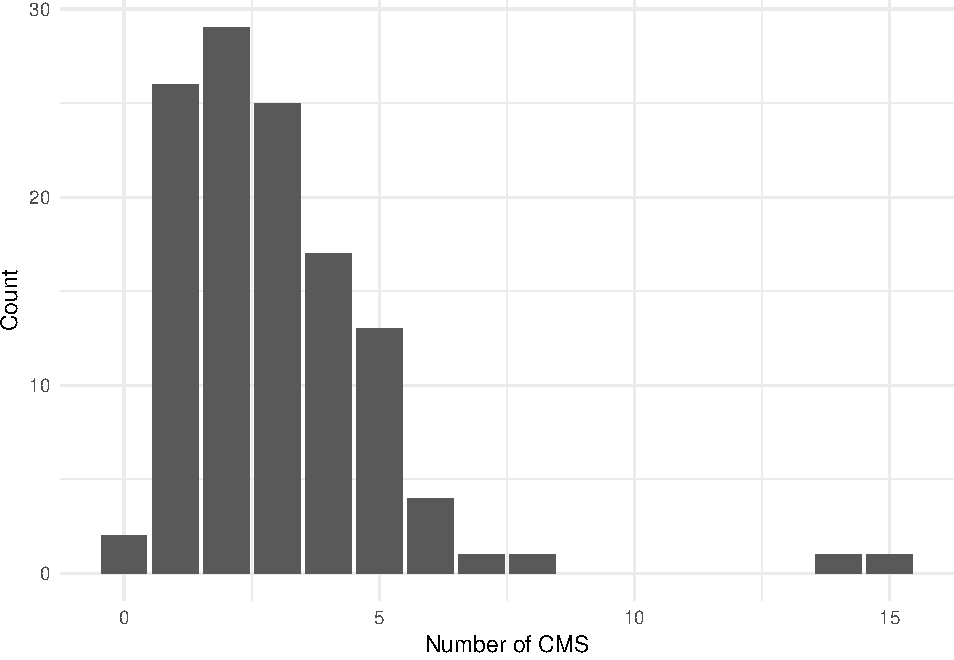
\includegraphics[width=.5\linewidth]{STfFP-Workbook_files/figure-latex/cmspois-1} 

}

\caption{Distribution of the maximum number of CMS for a randomly selected bullet compared to 118 known lands approximately follows a Poisson distribution.}\label{fig:cmspois}
\end{figure}

\section{Statistical Inference -
Estimation}\label{statistical-inference---estimation}

Recall from Section \ref{definitions}:

\begin{itemize}
\tightlist
\item
  The \_\_\_\_\_\_\_\_\_\_\_\_\_ is the universe of objects of interest.
  \vspace{.1in}
\item
  The \_\_\_\_\_\_\_\_\_\_\_\_\_ is comprised of the objects available
  for study. \vspace{.1in}
\item
  \_\_\_\_\_\_\_\_\_\_\_\_\_ is deductive: use knowledge about the
  population to make statements describing the sample \vspace{.1in}
\item
  \_\_\_\_\_\_\_\_\_\_\_\_\_ is inductive: use knowledge about the
  sample to make statements describing the population \vspace{.1in}
\item
  Probability and statistics are used together! \vspace{.1in}

  \begin{enumerate}
  \def\labelenumi{\arabic{enumi}.}
  \tightlist
  \item
    Build or assume a \_\_\_\_\_\_\_\_ for a population \vspace{.1in}
  \item
    Assess the \_\_\_\_\_\_\_\_\_ using the model \vspace{.1in}
  \item
    Refine the model, return to step 2.
  \end{enumerate}
\end{itemize}

\subsection{Background}\label{background}

A \_\_\_\_\_\_\_\_\_\_\_\_ is a numerical characteristic of the
population, e.g.~the population mean. Statistical methods are usually
concerned with learning about population parameters from
\_\_\_\_\_\_\_\_\_\_\_\_\_\_\_\_\_\_\_\_\_.

Note: The mean of a \emph{sample} and the mean of a \emph{population}
are differenct concepts. The mean of a sample can be calculated exactly,
while the mean of a population is (usually) unknown, because there are
too many objects in the population to record and calculate the mean.

The idea underlying statistical inference is that we can apply laws of
probability to draw \_\_\_\_\_\_\_\_\_\_ about a population from a
sample. This process is briefly summarized below:

\begin{itemize}
\tightlist
\item
  Observe \_\_\_\_\_\_\_\_\_ mean \vspace{.1in}
\item
  If we have a ``good'' sample this sample mean should be close to the
  \_\_\_\_\_\_\_\_\_\_\_ mean. \vspace{.1in}
\item
  The laws of \_\_\_\_\_\_\_\_\_\_\_\_ tell us how close we can expect
  them to be.
\end{itemize}

For example, suppose we are interested in the average height of the
adult population in the U.S.

\begin{itemize}
\tightlist
\item
  Population: \_\_\_\_\_\_\_\_\_\_\_\_\_\_\_ \vspace{.1in}
\item
  Sample: \_\_\_\_\_\_\_\_\_\_\_\_\_\_\_ \vspace{.1in}
\item
  We can take the average height of everyone here and use this sample
  \_\_\_\_\_\_\_\_\_\_\_ to make \_\_\_\_\_\_\_\_\_\_\_ about the
  \_\_\_\_\_\_\_\_\_\_\_\_ mean of all U.S. adults.
\item
  Note: This approach will work if our sample is a \_\_\_\_\_\_\_\_\_
  sample from the population. This assumption may be questionable, so it
  should be verified.
\end{itemize}

The \emph{goal} of statistical inference is \_\_\_\_\_\_\_\_\_\_\_\_
about a \_\_\_\_\_\_\_\_\_\_\_\_\_\_. Different possible parameters are:
\vspace{.1in}

\begin{itemize}
\tightlist
\item
  Mean
\item
  Variance
\item
  Proportion
\end{itemize}

We can also make different types of inferential statements, depending on
what question we are trying to answer and how we are going to report our
results. We will talk about:

\begin{itemize}
\tightlist
\item
  \_\_\_\_\_\_\_\_\_\_\_\_ estimate: an estimate of a parameter value
  \vspace{.1in}
\item
  \_\_\_\_\_\_\_\_\_\_\_\_ estimate: a range of plausible values for a
  parameter \vspace{.1in}
\item
  Hypothesis \_\_\_\_\_\_\_\_\_\_\_\_: examine a specific hypothesis
  about the true value of a parameter
\end{itemize}

When you want to do statistical inference, it is always inportant to
look at your sample data before proceeding directly to inference. We do
this because we want to

\begin{enumerate}
\def\labelenumi{\arabic{enumi}.}
\tightlist
\item
  See general \_\_\_\_\_\_\_\_\_\_\_\_\_ in the data \vspace{.1in}
\item
  Get an idea of the \_\_\_\_\_\_\_\_\_\_\_ of the distribution of the
  data \vspace{.1in}
\item
  Identify \_\_\_\_\_\_\_\_\_\_\_\_ values and/or errors.
\end{enumerate}

How we look at our data to check for these three things? If our data are
\_\_\_\_\_\_\_\_\_\_\_\_\_, we look at a table of frequencies or a bar
chart of the different outcomes. If our data are
\_\_\_\_\_\_\_\_\_\_\_\_, we look at histograms of the values, or
numerical summaries such as mean, median, standard deviation, or
percentiles.

A quick example shows why it can be important to examine your data
before a formal statistical analysis:

\begin{itemize}
\tightlist
\item
  Suppose the data are (19,20,21,22,23). Then, the mean is
  \(\frac{19+20+21+22+23}{5} = 21\), the median is 21, and the standard
  deviation is 1.58.
\item
  But what if the data you receive are (19,20,21,22,93)? Then, the mean
  is \(\frac{19+20+21+22+93}{5} = 35\), the median is 21, and the
  standard deviation is 32.4.
\item
  There could have been a typo, or someone interpreted some handwriting
  wrong, etc. The moral of the story is ALWAYS look at your data first!
\end{itemize}

\subsection{Point Estimation}\label{point-estimation}

An \_\_\_\_\_\_\_\_\_\_ is a rule for estimating a population
\_\_\_\_\_\_\_\_\_\_ from a sample. We evaluate the quality of the
estimator by considering two key properties:

\begin{itemize}
\tightlist
\item
  Bias: how close \_\_\_\_\_\_\_\_\_\_\_\_\_\_\_\_ an estimator is to
  the true population mean \vspace{.1in}
\item
  Variability: how \_\_\_\_\_\_\_\_\_\_ is the estimate?
\end{itemize}

For the population mean, we might use sample mean as an estimator
because it has \_\_\_\_\_ bias and \_\_\_\_\_\_\_\_ variability is the
sample is \_\_\_\_\_\_\_\_\_. There are other possible estimators for
the mean such as:

\begin{itemize}
\tightlist
\item
  The median (good for skewed data or data with outliers)
\item
  The midrange (\(\frac{\max + \min}{2}\))
\item
  47 (obviously this is just guessing and is not advised)
\end{itemize}

Let \(\theta\) denote an unknown population parameter that we wish to
estimate. The letter \(\theta\) represents the true value of the
parameter. In Figure \ref{fig:theta1}, we see what would happen in many
repeated attempts to estimate \(\theta\) using estimators with different
properties.

\begin{figure}[h]

{\centering 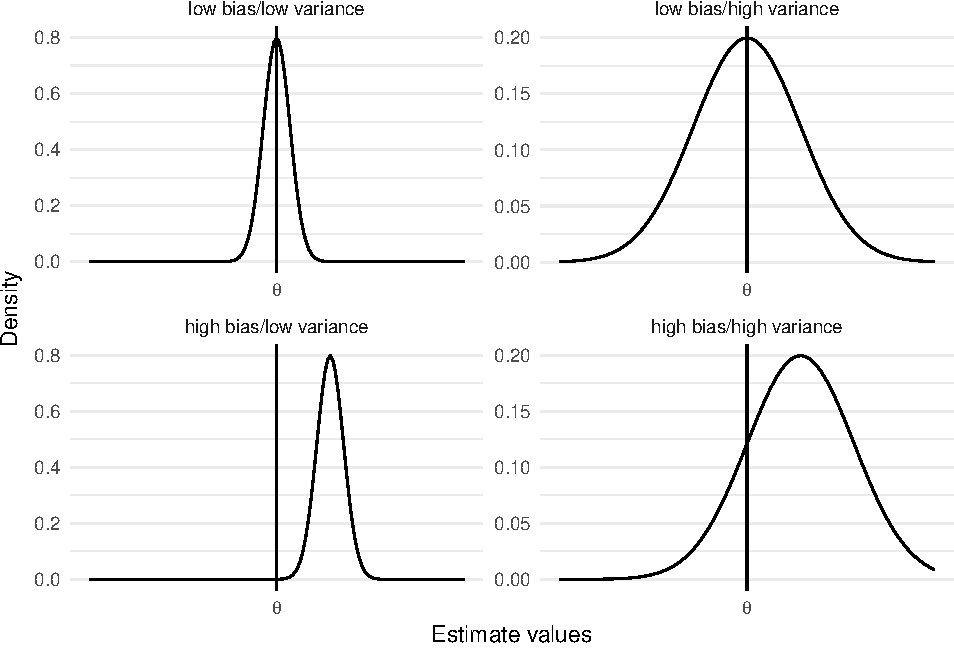
\includegraphics[width=.99\linewidth]{STfFP-Workbook_files/figure-latex/theta1-1} 

}

\caption{The curve in each plot shows the distribution of estimates we would see under each condition shown.}\label{fig:theta1}
\end{figure}

\subsection{Standard Errors}\label{standard-errors}

One limitation of just providing a point estimate is that it doesn't
give us any indication of \_\_\_\_\_\_\_\_\_\_\_\_\_. As we saw in
Figure \ref{fig:theta1}, a point estimate alone can be very different
from the true mean. We can do better than this!

The \_\_\_\_\_\_\_\_\_\_\_\_\_\_\_\_\_\_\_\_\_\_\_\_\_\_\_ of an
estimator measures the uncertainty in our estimate. When looking at a
summary statistic, like mean, median, or percentiles, that statistic is
also a \_\_\_\_\_\_\_\_\_\_\_\_\_\_\_\_\_ quantity. This means that if
we had observed a different set of sample values, we would observe
different values of the summary statistics. The idea of standard error
is similar to the idea of standard deviation. Both are measures of
spread, or variability. The difference is that standard deviation is a
measure of variability of a sample or population, while standard error
is a measure of variability of an \_\_\_\_\_\_\_\_\_\_\_\_\_\_\_.

Consider a population with that is normally distributed with mean 100
and standard deviation 15. Recall from Section \ref{normal} that 95\% of
observations from a normal distribution fall within two standard
deviations of the mean. So, in this example we expect 95\% of
observations to be between 70 and 130. This distribution is shown on
left in Figure \ref{fig:sampdist}. Now suppose we want to look at the
distribution of the \emph{estimates} of the population mean from several
samples. This will demonstrate the idea of standard error, using sample
size of \(n=25\). The formula to compute standard error is:

\[se = \frac{}{\sqrt{\quad}}\]

The standard error for this example is \(\frac{15}{\sqrt{25}} = 3\). The
mean of a sample of size 25 from this population should be about
\_\_\_\_\_\_\_\_. And about 95\% of the time, the sample mean will be
between \_\_\_\_\_ and \_\_\_\_\_. This distribution is shown on right
in Figure \ref{fig:sampdist}.

\begin{figure}[h]

{\centering 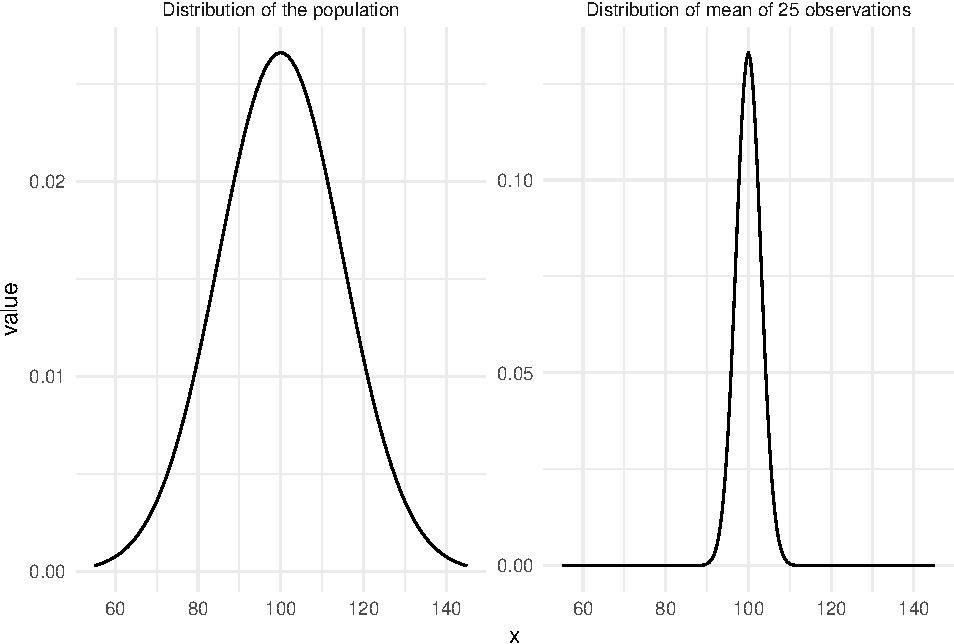
\includegraphics[width=.99\linewidth,height=3in]{STfFP-Workbook_files/figure-latex/sampdist-1} 

}

\caption{On the left, the distribution of the population, which is distributed N(100,15). On the right, the distribution of the sample mean for samples of size 25 from the populations, which is distributed N(100,3).}\label{fig:sampdist}
\end{figure}

\subsection{Sample Size}\label{sample-size}

The size of a sample plays a \emph{critical} role in determining how
accurate we can be. Again, consider a population with distribution
\(N(100,15)\). We can use \_\_\_\_\_\_\_\_\_\_ to examine the effect of
sample size. We simulate samples from a normal distribution with mean
100 and standard deviation 15. We use four different sample sizes: 10,
25, 50, and 100. We take 500 samples of each size and compute the mean
for each sample, leaving us with 2,000 means that we have calculated. We
show histograms of the means of these samples for each sample size in
Figure \ref{fig:sims}.

\begin{figure}[h]

{\centering 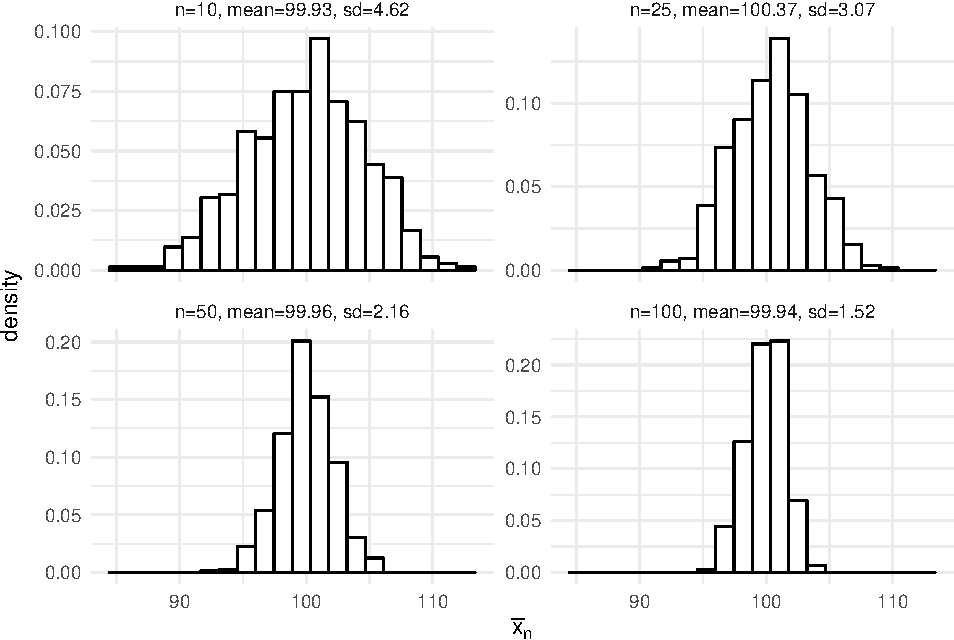
\includegraphics[width=.99\linewidth]{STfFP-Workbook_files/figure-latex/sims-1} 

}

\caption{How does sample size affect the sampling distribution? As sample size increases, the standard error decreases, so the distribution of sample means becomes more narrow.}\label{fig:sims}
\end{figure}

\subsection{Interval Estimation}\label{interval-estimation}

A \_\_\_\_\_\_\_\_\_\_\_ interval is an interval based on sample data
that, with some specified confidence \_\_\_\_\_\_\_\_\_, contains a
population parameter. Essentially, a confidence interval takes a
\_\_\_\_\_\_\_\_\_\_\_ estimate and then adds some information about
\_\_\_\_\_\_\_\_\_\_\_\_\_\_. Typically, we get an approximate
\_\_\_\_\_\% confidence interval for a quantity by taking a point
estimate and adding and subtracting 2 standard errors from it.

The most well-established procedures for finding confidence intervals
are those related to drawing conclusion about the mean of a
\_\_\_\_\_\_\_\_\_\_\_ population. Suppose that we have acquired a
random sample of \(n\) observations from a normal population.

\begin{itemize}
\tightlist
\item
  \textbf{Point} estimate: the natural point estimate of the population
  mean is the sample mean, as we've seen already. The sample mean is
  often denoted by \_\_\_\_\_. To calculate the sample mean, simple add
  up all the values and divide by the number of values you have, \(n\).
  In mathematical notation this is written:
\end{itemize}

\[\overline{X} = \frac{1}{n} \cdot \sum\limits_{i=1}^n X_i\]

\begin{itemize}
\tightlist
\item
  \textbf{Interval} estimate: denote the standard error of the sample
  mean by \(SE(\overline{X})\), and the standard deviation of the
  population by \(SD(\text{population})\). Then, compute the standard
  error by:
\end{itemize}

\[ SE(\overline{X}) = \frac{SD(\text{population})}{\sqrt{n}}\] Then, an
approximate 95\% confidence interval is computed:

\begin{equation}\label{eq:ci}
\overline{X} \pm 2 \cdot SE(\overline{X})
\end{equation}

A key result is that these procedures for point and interval estimation
work well even if the population does \textbf{not} follow a
\_\_\_\_\_\_\_\_\_\_\_ distribution \textbf{as long as the sample is
\_\_\_\_\_\_\_\_\_\_\_}.

For example, suppose there are 10 glass fragments found at a crime
scene, and the concentration of aluminum in each one is measured. The
mean aluminum concentration of the sample was 0.73 and the standard
deviation was 0.04. The standard error is thus:

\[ SE(\overline{X}) = \frac{}{\sqrt{\quad}} = 0.013\]

The approximate 95\% confidence interval for the mean aluminum
concentration in the crime scene window is:

\[ 0.73 \pm 1.96 \cdot 0.013 = (\_\_\_,\_\_\_)\]

The \emph{interpretation} of the confidence interval is important: 95\%
of the intervals \_\_\_\_\_\_\_\_\_ in this way will contain the
\_\_\_\_\_\_ population parameter.

\section{Statistical Inference - Hypothesis
Testing}\label{statistical-inference---hypothesis-testing}

Sometimes we wish to formally \_\_\_\_\_\_\_\_\_ a hypothesis about a
population parameter. The hypothesis to be evaluated is known as the
\_\_\_\_\_\_\_ hypothesis. This hypothesis is usually the status quo, or
what is assumed to be true. When hypothesis testing we look for evidence
\_\_\_\_\_\_\_\_\_ the null. There is also a an \_\_\_\_\_\_\_\_\_\_\_\_
or research hypothesis that helps us design the test. If we
\_\_\_\_\_\_\_\_\_ the null hypothesis, then we say that we have a
statistically \_\_\_\_\_\_\_\_\_\_\_\_ result.

As with anything in life, errors are possible in hypothesis testing.
There are two main typs of errors that we care about:

\begin{enumerate}
\def\labelenumi{\arabic{enumi}.}
\tightlist
\item
  Type I: \_\_\_\_\_\_\_\_\_\_ the null hypothesis when it is
  \_\_\_\_\_\_\_\_\_. (false positive) \vspace{.1in}
\item
  Type II: \_\_\_\_\_\_\_\_\_\_\_\_\_\_\_\_\_\_\_\_ the null hypothesis
  when it is \_\_\_\_\_\_\_\_\_. (false negative) \vspace{.1in}
\end{enumerate}

Of these two errors, Type I error is often considered more serious. We
only want to \_\_\_\_\_\_\_\_\_\_\_ the null hypothesis is there is
\emph{strong} evidence against it. These statistical testing ideas are
closely related to concepts in the
\_\_\_\_\_\_\_\_\_\_\_\_\_\_\_\_\_\_\_\_\_\_\_:

\begin{itemize}
\tightlist
\item
  The null hypothesis: the defendant is \_\_\_\_\_\_\_\_\_\_\_
  \vspace{.1in}
\item
  The alternative hypothesis: the defendant is \_\_\_\_\_\_\_\_\_\_
  \vspace{.1in}
\item
  In court, a Type I error is to find guilty when the defendant is
  \_\_\_\_\_\_\_\_\_\_\_\_ \vspace{.1in}
\item
  In court, a Type II error is to find innocent when the defendant is
  \_\_\_\_\_\_\_\_\_\_\_\_
\end{itemize}

Ultimately, the basic idea of hypothesis testing is to compute a
\_\_\_\_\_\_\_\_\_\_\_\_\_\_\_\_\_\_ that measures ``distance'' between
the \_\_\_\_\_\_ we have collected and what we expect under the
\_\_\_\_\_\_ hypothesis. Typically, we use a test statistic of the form:

\begin{equation}\label{eq:teststat}
\frac{\text{point estimate} - \text{null hypothesis value}}{SE(\text{estimate})}
\end{equation}

This test statistic can be interpreted as the number of
\_\_\_\_\_\_\_\_\_\_\_\_\_\_\_\_\_ the sample estimate is from the
\_\_\_\_\_\_\_\_\_\_\_\_\_ value under the null hypothesis.

A common way to to summarize hypothesis tests is by attaching a
\_\_\_\_\_\_\_\_\_\_\_ to the test statistic. This probability is called
a \_\_\_\_\_\_\_\_\_\_\_\_. The \(p\)-value of a hypothesis test gives
the probability that we would get data like that in our sample (or
something even more \_\_\_\_\_\_\_\_\_), given our assumption that the
null hypothesis is \_\_\_\_\_\_\_. This idea is demonstrated in Figure
\ref{fig:pvals}.

Small \(p\)-values mean that we have observed \_\_\_\_\_\_\_\_ data that
lead us to question the \_\_\_\_\_\_\_\_ hypothesis, which we have
\emph{assumed to be true}. Small \(p\)-values tell us that the sample
data are unlikely to happen by chance under the null. A \(p\)-value,
however, \emph{only} addresses the \_\_\_\_\_\_\_\_ hypothesis. It does
\emph{not} speak to the likelihood of the \_\_\_\_\_\_\_\_\_\_
hypothesis being true.

\begin{figure}[h]

{\centering 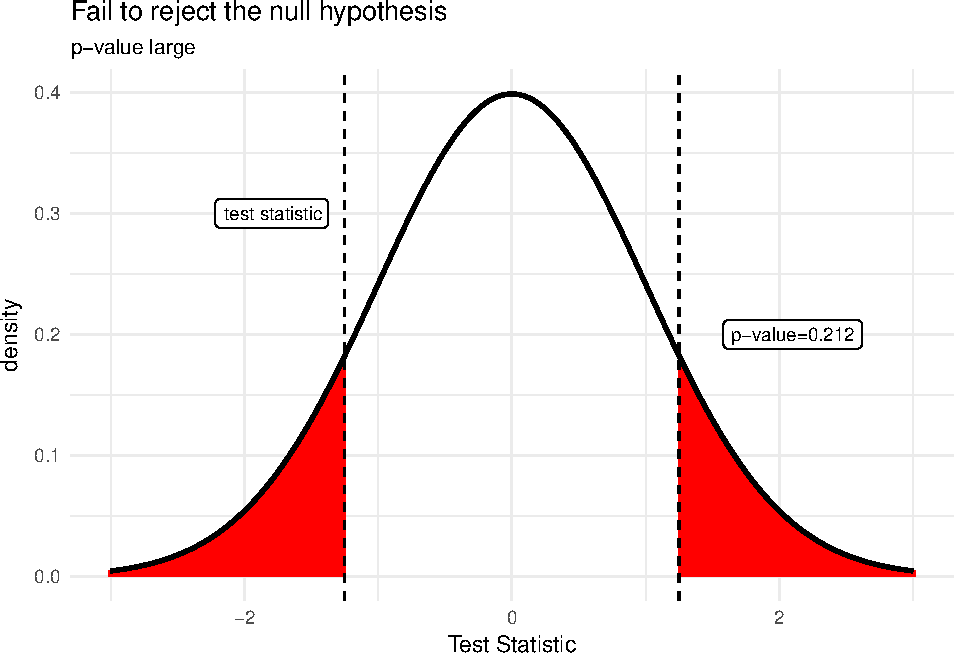
\includegraphics[width=.49\linewidth]{STfFP-Workbook_files/figure-latex/pvals-1} 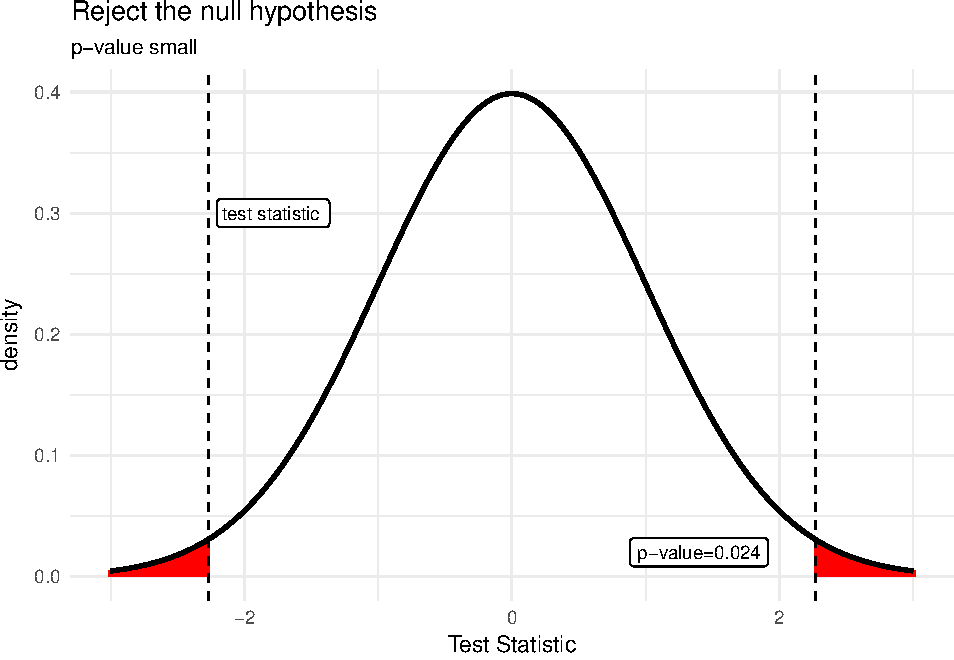
\includegraphics[width=.49\linewidth]{STfFP-Workbook_files/figure-latex/pvals-2} 

}

\caption{On the left, an example of a $p$-value that is large (test statistic small), leading us to fail to reject the null hypothesis. On the right, an example of a $p$-value that is small (test statistic large), leading us to reject the null hypothesis.}\label{fig:pvals}
\end{figure}

\subsection{Normal Data}\label{normal-data}

The most well-established hypothesis testing procedure is for testing a
hypothesis about the \_\_\_\_\_\_\_\_\_ of a \_\_\_\_\_\_\_\_\_\_\_\_
population. This population parameter is denoted \(\mu\). We can test
the hypothesis that the population mean, \(\mu\), is equal to some
specified values \(\mu_0\). The hypotheses for this test are:

\begin{itemize}
\tightlist
\item
  Null hypothesis - \(H_0 : \mu = \mu_0\) \vspace{.1in}
\item
  Alternative hypothesis - \(H_A : \mu \neq \mu_0\)
\end{itemize}

The test statistic, call it \(T\), to perform this hypothesis follows
the form of Equation \ref{eq:teststat}:

\begin{equation}\label{eq:Tnorm}
t = \frac{\_\_\_ - \_\_\_}{SE(\_\_\_)}
\end{equation}

The \(p\)-value for this hypothesis test is obtained from a \(t\)
distribution (see Figure \ref{fig:normt}) using software, a table of
values, or an online calculator. These hypothesis testing procedures
work well even if the population is \emph{not} normally distributed
\textbf{as long as the sample size is \_\_\_\_\_\_\_\_\_\_\_\_}.

\begin{figure}[h]

{\centering 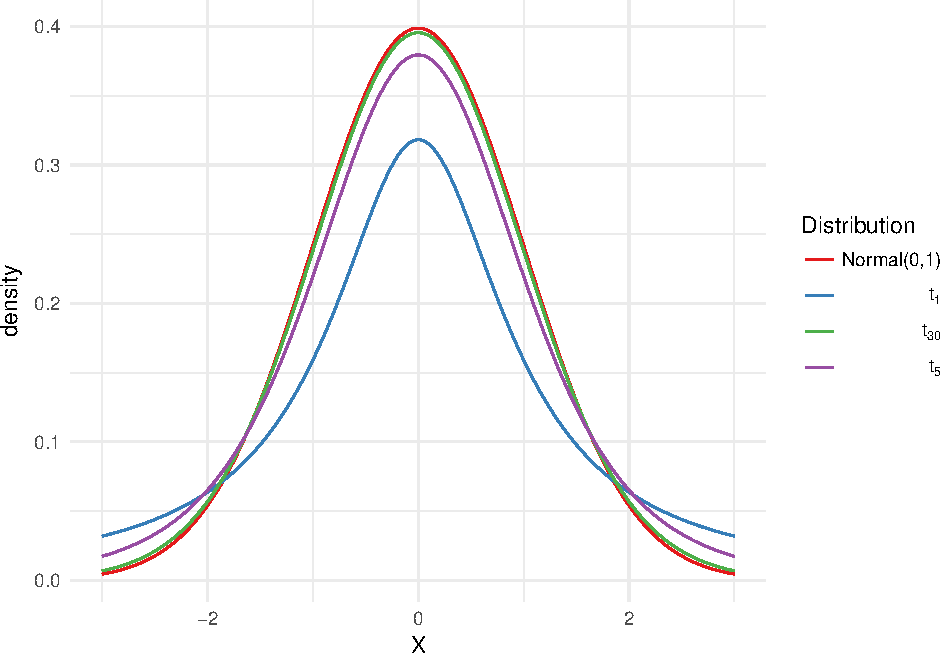
\includegraphics[width=.5\linewidth]{STfFP-Workbook_files/figure-latex/normt-1} 

}

\caption{The $t$ distribution is simlar to the Normal distribution (red line) is shape, but the tails are higher. As the sample size increases, the $t$ distribution approaches the the Normal distribution.}\label{fig:normt}
\end{figure}

\subsubsection{Example}\label{example}

Suppose we want to estimate the mean amount of a trace element for the
population of all bullets in Iowa. We get a random sample of 400 bullets
from the state.

\begin{itemize}
\tightlist
\item
  The sample mean concentration is \(\overline{X} = 55.5\) \vspace{.1in}
\item
  The sample standard deviation is \(s = 22.0\) \vspace{.1in}
\item
  The standard error of the mean is
  \(SE(\overline{X}) = \frac{22}{\sqrt{400}} = \frac{22}{20} = \_\_\_\_\)
\end{itemize}

Suppose we have reason to believe that Remington (mean = 58) is the main
producer in this area. We can check this idea with a hypothesis test.

\begin{itemize}
\tightlist
\item
  Null hypothesis - \(H_0 : \mu = 58\)
\item
  Alternative hypothesis - \(H_A : \mu \neq 58\)
\item
  Test statistic -
  \(t = \frac{\overline{X} - \mu_0}{SE(\overline{X})} = \frac{55.5-58}{1.10} = -2.27\)
\end{itemize}

The value of the test statistic is more than two standard errors away
from the mean under the null hypothesis. The exact \(p\)-value is 0.023.
This means that if the null hypothesis is true, then observing a value
2.27 standard errors or more away from the mean happens only 2.3\% of
the time. So, we reject our assumption that the population mean
concentration is 58.

We can also calculate a 95\% confidence interval for the mean using
Equation \ref{eq:ci}:

\[55.5 \pm 1.96\cdot 1.10 = (53.3, 57.7)\]

The hypothesized value (58) is is not in the 95\% confidence interval,
which also suggests that population mean concentration equal to 58 is
not possible.

\subsection{Confidence Intervals}\label{confidence-intervals}

There is a very close relationship between tests and interval estimates.
Recall that a confidence interval (CI) gives a range of plausible values
for the true population parameter, which here is the mean. A hypothesis
test evaluates whether a specified (\(\mu_0\)) is a
\_\_\_\_\_\_\_\_\_\_\_\_ value for the mean. A CI collects all values of
\(\mu_0\) that we would find plausible in a test.

Statistical hypothesis test are \emph{very} popular in practice.
Sometimes, they address the scientific question of interest, but often
they do not.\footnote{For more reading on this topic, consider this
  article from \emph{Nature}:
  \url{http://www.nature.com/news/psychology-journal-bans-p-values-1.17001}}

\subsection{Comparing Two Means}\label{comparing-two-means}

In section \ref{normal-data}, we discussed hypothesis testing methods
for one sample. In practice, we are often interested in comparing
\_\_\_\_\_\_ samples from \_\_\_\_\_ different populations. For now,
assume we have random samples from each of the two populations that we
are interested in. The test we want to do is a test for
\_\_\_\_\_\_\_\_\_\_\_\_\_\_ of parameters in the two populations.

\subsubsection{Example}\label{example-1}

Suppose, for example, that we have collected broken glass at a crime
scene, and glass fragments on a suspect. Define \(\mu_{scene}\) to be
the mean trace element level for population of glass at the scene.
Define \(\mu_{suspect}\) to be the mean element level for the population
of glass on the suspect. We can compare the means to address the
question of whether or not the glass fragments on the suspect could
plausibly have come from the crime scene.

Hypotheses:

\begin{itemize}
\tightlist
\item
  \(H_0 : \mu_{scene} \quad \_\_\_ \quad \mu_{suspect}\) \vspace{.1in}
\item
  \(H_A : \mu_{scene} \quad \_\_\_ \quad \mu_{suspect}\)
\end{itemize}

Suppose 10 glass fragments are taken from the glass found at the scene
(denote these by \(Y\)), and 9 fragments are found on the suspect
(denote these by \(X\)). Concentrations of a trace element were measured
in each fragment of glass. Summary values from the samples are:

\begin{itemize}
\tightlist
\item
  \(\overline{X} = 5.3\) \vspace{.1in}
\item
  \(s_X = 0.9\) \vspace{.1in}
\item
  \(SE(\overline{X}) = \frac{s_X}{\sqrt{n_X}} = \frac{0.9}{\sqrt{10}} = 0.28\)
  \vspace{.1in}
\item
  \(\overline{Y} = 5.9\) \vspace{.1in}
\item
  \(s_Y = 0.85\) \vspace{.1in}
\item
  \(SE(\overline{Y}) = \frac{s_Y}{\sqrt{n_Y}} = \frac{0.85}{\sqrt{9}} = 0.28\)
  \vspace{.1in}
\item
  Obeserved difference =
  \(\overline{X} - \overline{Y} = \_\_\_ - \_\_\_ = 0.6\) \vspace{.1in}
\item
  The standard error for the \emph{difference},
  \(\overline{X} - \overline{Y}\), is
  \[SE(\{\overline{X} - \overline{Y}\}) = \sqrt{SE(\overline{X})^2 + SE(\overline{Y})^2} = \sqrt{\_\_\_ + \_\_\_} = 0.4\]
\item
  The test statistic for this hypothesis test is:
  \[t = \frac{(\overline{X} - \overline{Y}) - 0}{SE(\{\overline{X} - \overline{Y}\})} = \frac{0.6}{0.4} = 1.5\]
\item
  The corresponding \(p\)-value for this statistic is 0.15.
\item
  So, we fail to reject the null hypothesis that the two glass
  population means are equal.
\item
  Interpretation is a \emph{key} issue. When we say we fail to reject
  the null, we are saying there is a possibility of a common source.
\end{itemize}

\subsection{Discussion}\label{discussion}

There are three key points for you to take away:

\begin{enumerate}
\def\labelenumi{\arabic{enumi}.}
\tightlist
\item
  Hypothesis testing does \emph{not} treat the two hypotheses
  \_\_\_\_\_\_\_\_\_\_\_\_\_. The null hypothesis is given priority.
  This is appropriate when there is reason to \_\_\_\_\_\_\_\_\_\_\_ the
  null hypothesis until there is significant evidence
  \_\_\_\_\_\_\_\_\_\_\_\_\_\_ it. We don't necessarily always want this
  to be the case. (We will discuss this more later on in a forensic
  context.) \vspace{.1in}
\item
  The \(p\)-values that result from hypothesis tests depend heavily on
  the sample size. If you have the same \_\_\_\_\_\_\_ and standard
  deviation, but \_\_\_\_\_\_\_\_\_\_\_ the sample size, the result will
  me more significant, due to the sample size alone. \vspace{.1in}
\item
  Interpreting the results of the hypothesis test can be tricky. If we
  \_\_\_\_\_\_\_\_\_\_ the null hypothesis, this does not necessarily
  mean that we have found an important difference in the context of our
  problem. In addition
  \_\_\_\_\_\_\_\_\_\_\_\_\_\_\_\_\_\_\_\_\_\_\_\_\_\_ the null
  hypothesis does not necessarily mean the null hypothesis is true.
\end{enumerate}

\section{Overview of Statistical
Preliminaries}\label{overview-of-statistical-preliminaries}

\begin{itemize}
\tightlist
\item
  We reviewed the basics of probability

  \begin{itemize}
  \tightlist
  \item
    Probability is the language of uncertainty
  \item
    It is important to understand what is being assumed when talking
    about probability
  \item
    For instance, the probability of having disease given a positive
    test is different than the probability of having a positive test
    given the disease
  \item
    Probability distributions describe the variability in a population
    or in a series of measurements
  \end{itemize}
\item
  We reviewed basics of statistical inference

  \begin{itemize}
  \tightlist
  \item
    Statistical inference uses sample data to draw conclusions about a
    population
  \item
    Point estimation, interval estimation, and hypothesis tests are main
    tools
  \item
    It is critical that our procedures account for variation that could
    be observed due to chance
  \end{itemize}
\end{itemize}

\chapter{Statistics for Forensic
Science}\label{statistics-for-forensic-science}

In this section, we will first discuss a brief review of probability and
statistics. Then, we will outline the forensic examination and discuss
where probability and statistics can be added, and two different
approaches to consider.

\section{Brief Review of Probability and
Statistics}\label{brief-review-of-probability-and-statistics}

\begin{itemize}
\tightlist
\item
  Probability is\ldots{}

  \begin{itemize}
  \tightlist
  \item
    the language for describing uncertainty.
  \item
    a number, always between 0 and 1, to describe the likelihood of an
    event.
  \item
    dependent on the information available (information conditioned on)
  \item
    useful for deducing likely values for individuals or samples from
    given or hypothesized information about the population
  \end{itemize}
\item
  Probability distributions\ldots{}

  \begin{itemize}
  \tightlist
  \item
    suppose we have a \emph{random} quantity, like a trace element
    concentration in a glass fragment.
  \item
    give possible values and relative likelihood of each value observed
    or observable.
  \end{itemize}
\item
  Statistics\ldots{}

  \begin{itemize}
  \tightlist
  \item
    draws inferences about a population (usually some characteristic of
    the population) based on sample data.
  \item
    relies on careful definition of the ``population'' of interest.
  \item
    relies on the method of data collection.
  \item
    is made up of a variety of \emph{inference} procedures, like\ldots{}

    \begin{itemize}
    \tightlist
    \item
      point estiamtes,
    \item
      confidence intervals, and
    \item
      hypothesis tests.
    \end{itemize}
  \end{itemize}
\end{itemize}

\section{The Forensic Examination}\label{the-forensic-examination}

As you know there are a range of question that arise in forensic
examinations, such as source conclusion, the timing of events, and cause
\& effect. We focus in this section on sources conclusions.

The evidence, which we will denote \(E\), are items or objects found at
the crime scene and on a suspect. \(E\) can also denote the measurements
of these items. For evidence found at the crime scene, we will
occasionally write \_\_\_\_\_\_\_, and for evidence found on the suspect
or in the suspect's possession, we will occasionally write \_\_\_\_\_\_.
There is also other information available to us, denoted \(I\), such as
the race of the perpetrator (according to a witness) or evidence
substrate.

In the source conclusions piece of the forensic examination, we can
divide the possible events into two groups:

\begin{itemize}
\tightlist
\item
  \(S\) : the items from the crime scene and from the suspect have
  \_\_\_\_\_\_\_\_\_\_ source. In other words, the suspect is the
  \_\_\_\_\_\_\_\_\_\_\_ of a crime scene item. \vspace{.1in}
\item
  \(\overline{S}\) : the items from the crime scene and from the suspect
  \_\_\_\_\_\_\_\_\_\_\_ have common source.
\end{itemize}

The goal of the forensic examination is the assessment of evidence.
There are two primary questions:

\begin{enumerate}
\def\labelenumi{\arabic{enumi}.}
\tightlist
\item
  Do the items found at the crime scene and with the suspect appear to
  have a common source?
\item
  How unusual is it to observe source agreement \emph{by chance}?
\end{enumerate}

Obviously, there are many different types of forensic evidence:

\begin{itemize}
\tightlist
\item
  biological evidence (such as blood type or DNA)
\item
  glass fragments
\item
  fibers
\item
  latent prints
\item
  shoe prints or tire tracts
\item
  and others
\end{itemize}

Different probability \& statistics related issues will inevitably arise
for different evidence types. For example:

\begin{itemize}
\tightlist
\item
  Discrete and continuous variables are treated differently.
\item
  What information is available about the probability distribution of
  observable measurements?
\item
  A reference database may or may not exist.
\item
  What role does the manufacturing process play in ability to make a
  match?
\end{itemize}

The Daubert standard\footnote{\emph{Daubert v. Merrell Dow
  Pharmaceuticals}, 509 U.S. 579} identifies the the judge as a
\_\_\_\_\_\_\_\_\_\_\_\_\_\_\_\_\_\_\_\_\_ to determine the
admissibility of expert scientific testimony. In order to determine
admissibility, the judge can apply \_\_\_\_\_\_\_\_\_\_\_\_\_ factors:
\vspace{.1in}

\begin{itemize}
\tightlist
\item
  The theory or method should be \_\_\_\_\_\_\_\_\_\_\_ \vspace{.1in}
\item
  The theory or method should be subject to \_\_\_\_\_\_\_\_\_\_\_\_ and
  \_\_\_\_\_\_\_\_\_\_\_\_\_. \vspace{.1in}
\item
  There are known or potential \_\_\_\_\_\_\_\_\_\_ rates.\vspace{.1in}
\item
  The theory or method has \_\_\_\_\_\_\_\_\_\_\_\_ and
  controls.\vspace{.1in}
\item
  The theory or method is generally \_\_\_\_\_\_\_\_\_\_\_\_ by the
  \_\_\_\_\_\_\_\_\_\_\_\_\_ scientific community.
\end{itemize}

The National Research Council (Committee on Identifying the Needs of the
Forensic Sciences Community and Council
(\protect\hyperlink{ref-nrc09}{2009})) found:\vspace{.1in}

\begin{itemize}
\tightlist
\item
  \_\_\_\_\_\_\_\_\_\_\_\_\_\_\_ provider community (federal, state, \&
  local) \vspace{.1in}
\item
  \_\_\_\_\_\_\_\_\_\_\_\_\_\_\_ across disciplines \vspace{.1in}
\item
  Lack of \_\_\_\_\_\_\_\_\_\_\_\_\_\_\_\_\_\_\_\_ in practices
  \vspace{.1in}
\item
  Insufficient \_\_\_\_\_\_\_\_\_\_\_\_\_\_\_\_\_ \vspace{.1in}
\item
  Questions underlying \_\_\_\_\_\_\_\_\_\_\_\_\_\_\_\_ basis for some
  conclusions
\end{itemize}

This led to \emph{single source} DNA's emergence as a
\_\_\_\_\_\_\_\_\_\_\_\_\_\_\_\_\_\_\_\_\_\_\_\_\_.

In 2016, the President's Council of Advisors on Science and Technology
released a report on the state of forensic science. (Advisors on Science
\& Technology (\protect\hyperlink{ref-pcast}{2016})). This
report\ldots{} \vspace{.1in}

\begin{itemize}
\tightlist
\item
  focused on the \_\_\_\_\_\_\_\_\_\_\_ of \_\_\_\_\_\_\_\_\_\_\_\_
  matching disciplines: \vspace{.1in}

  \begin{itemize}
  \tightlist
  \item
    examined foundational validity and the use of
    \_\_\_\_\_\_\_\_\_\_\_\_\_\_\_\_\_\_\_\_\_ studies \vspace{.1in}
  \item
    examined validity as \_\_\_\_\_\_\_\_\_\_\_, including information
    at the examiner level.
  \end{itemize}
\end{itemize}

The forensic science community as a whole is a community in transition.
The National Commission on Forensic Science, which was established in
2013 to advise the U.S. Attorney General, was not renewed for a third
term after its second term expired on April 23, 2017.\footnote{\url{https://www.washingtonpost.com/local/public-safety/sessions-orders-justice-dept-to-end-forensic-science-commission-suspend-review-policy/2017/04/10/2dada0ca-1c96-11e7-9887-1a5314b56a08_story.html?utm_term}=.858a461dec18}
To accompany the end of this commission, the Department of Justice (DOJ)
released a call for comments on advancing forensic science, with
comments closing on June 9, 2017.\footnote{\url{https://www.justice.gov/opa/press-release/file/956146/download}}

There are additional federal organizations that are also involved in
advancing the field of forensic science. For instance, Organization of
Scientific Area Committees (OSAC) for Forensic Sciences is also a part
of NIST.\footnote{\url{https://www.nist.gov/topics/forensic-science/organization-scientific-area-committees-osac}}
In addition, the NIJ and NIST have forensic Centers of Excellence, the
Forensic Technology Center of Excellence\footnote{NIJ:
  \url{https://forensiccoe.org/}} (FTCoE) and the Center for Statistics
and Applications in Forensic Evidence.

\section{Common Approaches to Assessing Forensic
Evidence}\label{common-approaches-to-assessing-forensic-evidence}

In this section, we consider the two primary approaches to assessing
forensic evidence: expert assessment based on experience and training,
and statistical approaches, including statistical testing and likelihood
ratio based approaches.

Ultimately, the goal of the collaboration between academics and
practitioners is to come to a combination of the two as the gold
standard for assessing forensic evidence.

\subsection{Significance Testing / Coincidence
Probability}\label{significance-testing-coincidence-probability}

One common statistical approach\footnote{This approach is also known as
  the \emph{comparison/significance approach}.} solves the forensic
problem in two stages:

\begin{enumerate}
\def\labelenumi{\arabic{enumi}.}
\tightlist
\item
  First, we determine if the crime scene and suspect objects
  \_\_\_\_\_\_\_\_ on characteristic of \_\_\_\_\_\_\_\_\_\_. This is
  typically done using a hypothesis or a significance \_\_\_\_\_\_\_.
  \vspace{.1in}
\item
  Second, we assess the \_\_\_\_\_\_\_\_\_\_\_\_\_\_\_\_ of thi
  agreement by finding the likelihood of such agreement occurring by
  \_\_\_\_\_\_\_\_.
\end{enumerate}

\textbf{Note}: DNA analysis can be categorized in this way, but is
usually thought of as a \emph{likelihood ratio} approach. See Section
\ref{likelihood-ratio} for more.

In the significance testing or coincidence probability approach,
determining agreement is straightforward for \_\_\_\_\_\_\_\_ data like
blood type or gender. There are still \_\_\_\_\_\_\_\_\_\_\_\_\_ in
these cases due to the possibility of laboratory or measurement error.
Usually, it is easier or more straightforward to think about discrete
data in terms of the likelihood ratio. Again, see Section
\ref{likelihood-ratio} for more. Statistical significance tests can also
be used for \_\_\_\_\_\_\_\_\_\_\_\_\_ data like trace element
concentrations (e.g., in glass fragments).

For this approach, the testing procedure is outlined below:
\vspace{.1in}

\begin{enumerate}
\def\labelenumi{\arabic{enumi}.}
\tightlist
\item
  \_\_\_\_\_\_\_\_\_\_\_\_\_\_\_\_ each object by a \_\_\_\_\_\_\_
  value. For example, consider the mean trace element concentration in a
  \emph{population} of glass fragments. This is the \_\_\_\_\_\_\_\_\_\_
  mean in statistics terminology: one mean for glass from the crime
  scene, one mean for glass from the suspect) \vspace{.1in}
\item
  Obtain \_\_\_\_\_\_\_\_\_ values from the \_\_\_\_\_\_\_\_\_\_\_
  object. \vspace{.1in}
\item
  Obtain \_\_\_\_\_\_\_\_\_ values from the \_\_\_\_\_\_\_\_\_\_\_
  object. \vspace{.1in}
\item
  Use the sample values from steps 2-3 to test the
  \_\_\_\_\_\_\_\_\_\_\_\_\_\_\_ that the two objects have the same
  population \_\_\_\_\_\_\_\_\_\_. The common tool for testing is the
  \(t\)-test demonstrated earlier in Section \ref{comparing-two-means}.
  \vspace{.1in}
\item
  Summarize the test with the \(p\)-value, the \_\_\_\_\_\_\_\_\_\_\_ of
  data like the observed data or more extreme, assuming population means
  are the same. \vspace{.1in}
\item
  A small \(p\)-value, typically small means \(p < .05\) or \_\_\_\_\_,
  indicates there is no agreement between the two objects. If the
  \(p\)-value is larger, we can't \_\_\_\_\_\_\_\_\_\_\_ the hypothesis
  that the two means are equal.\footnote{But is this evidence that they
    came from the same population\ldots{}?}
\end{enumerate}

\subsubsection{Examples}\label{examples-4}

First, consider two glass samples: one from a crime scene, and one from
a sample recovered from the suspect. These data can be found in Curran
et al. (\protect\hyperlink{ref-curranetal}{1997}). The null hypothesis
(\(H_0\)) is that the two samples come from the same source, and the
alternative hypothesis (\(H_A\)) is that the two samples are from
different sources.

\begin{itemize}
\item
  Five measurements of \_\_\_\_\_\_\_\_\_\_\_\_ concentration in crime
  scene sample: \[0.751, 0.659, 0.746, 0.772, 0.722\]
\item
  Five measurements of \_\_\_\_\_\_\_\_\_\_\_\_ concentration in
  recovered sample: \[0.752, 0.739, 0.695, 0.741, 0.715\]
\item
  Sample means:

  \begin{itemize}
  \tightlist
  \item
    Crime Scene: 0.730
  \item
    Recovered Sample: 0.728
  \end{itemize}
\item
  Standard errors

  \begin{itemize}
  \tightlist
  \item
    Crime Scene: \(\frac{0.0435}{\sqrt{5}}=0.019\)
  \item
    Recovered Sample: \(\frac{0.023}{\sqrt{5}}=0.010\)
  \end{itemize}
\item
  Test statistic (see Section \ref{comparing-two-means}):
  \[\frac{0.730 - 0.728}{\sqrt{0.019^2 + 0.010^2}} = \frac{0.002}{0.0215} = 0.0931 \approx 0.1\]
\item
  \(p\)-value = 0.70 \(\Rightarrow\) fail to reject the null hypothesis
  that the two samples come from the same source
\end{itemize}

In fact, ground truth is known here: these measurements did come from
the same bottle.

Next, consider a different recovered sample. Again, the data are from
Curran et al. (\protect\hyperlink{ref-curranetal}{1997}). The crime
scene sample remains the same as the prior example.

\begin{itemize}
\tightlist
\item
  Five measurements of aluminum concentration in the second recovered
  sample: \[0.929, 0.859, 0.845, 0.931, 0.915\]
\item
  Sample means:

  \begin{itemize}
  \tightlist
  \item
    Crime Scene: 0.730
  \item
    Recovered Sample: 0.896
  \end{itemize}
\item
  Standard errors

  \begin{itemize}
  \tightlist
  \item
    Crime Scene: \(\frac{0.0435}{\sqrt{5}}=0.019\)
  \item
    Recovered Sample: \(\frac{0.0408}{\sqrt{5}}=0.018\)
  \end{itemize}
\item
  Test statistic (see Section \ref{comparing-two-means}):
  \[\frac{0.730 - 0.896}{\sqrt{0.019^2 + 0.018^2}} = \frac{-0.166}{0.0262} = -6.38 \]
\item
  \(p\)-value = 0.0015 \(\Rightarrow\) Reject the null hypothesis that
  the two samples come from the same source.
\end{itemize}

In fact, ground truth is again known, and these two samples are from two
different bottles.

\subsubsection{Other Significance Testing
Approaches}\label{other-significance-testing-approaches}

Many other alternative, related methods exist for assessing forensic
evidence. For instance, 4-\(\sigma\) (4-sigma) methods create an
interval for each element in each sample, which are formed by taking the
mean concentration of each element \(\pm\) four standard errors of those
means. Then, check each interval for overlap, using ``control'' sample
to obtain an expected range and checking whether the ``test'' samples
are in/out of the control range. Hotelling's \(T^2\) (T-squared) test
compares all elements simultaneously to account for the within-sample
dependence.

There are some \textbf{technical} concerns about the aforementioned
procedures. The formal tests, the \(t\)-test and Hotelling's \(T^2\)
test, require assumptions about the probability distribution of the
data. In addition, univariate procedures such as the \(t\)-test are
repeated on multiple elements, and the existence of multiple comparisons
should be accounted for. Furthermore, univariate procedures ignore
information in the correlation of elements multivariate procedures (like
Hotelling's test) require large samples.

The bigger concerns with these procedures are \textbf{conceptual}.
First, significance tests do not treat the two hypotheses (equal means
vs.~unequal means) symmetrically:

\begin{itemize}
\tightlist
\item
  The null hypothesis, that the means are equal, is \emph{assumed} true
  unless the data \emph{rejects} the null hypothesis
\item
  Failing to reject the null in this hypothesis test setting is taken as
  evidence \emph{against} the suspect. This is the opposite of the
  courtroom setup, where failing to reject the null is taken as
  \emph{lack of} evidence against the suspect. Thus, the asymmetry of
  the null and alternative hypotheses is an issue here. In addition, the
  binary decision to reject the null fail to reject the null requires an
  arbitrary cutoff value. e.g.~Why 4\(\sigma\) rather than 3\(\sigma\)?
  Why \(p = 0.05\) rather than \(p = 0.01\) or \(p = 0.10\)? Lastly, the
  match decision from the hypothesis test is separated from assessment
  of the practical significance of the match. How different two samples
  are, according to the hypothesis test, may not correspond to the
  ground truth. e.g.~a large sample size will decrease the threshold for
  rejection, which could cause true matches to be misclassified as
  different sources if the within-population variation is large enough.
  And conversely, a small sample size will increase the rejection
  threshold and will be unable to distinguish true non-matches from
  matches because of a lack of information about the two truly different
  populations. 
\end{itemize}

\subsubsection{Alternatives to Significance
Tests}\label{alternatives-to-significance-tests}

Another route to investigate is \textbf{equivalence testing} instead of
significance testing. Equivalence testing changes the null hypothesis
and addresses the first concern regarding asymmetric hypostheses. The
Bayesian approach and the likelihood ratio approah address the other
concerns: these methods avoid the binary decision and the separation of
match and significance. We discuss these methods further later on in
Section \ref{likelihood-ratio} and focus on equivalence testing for now.

The usual hypotheis test assumes the null hypothesis is true until
proven otherwise. \textbf{Equivalence testing} is an alternative
approach that *assumes the population means are different. This becomes
the null hypothesis, but it also requires us to specify a
``practically'' important difference, \(\Delta\). We then write the
hypotheses as:

\begin{equation}\label{eq:et}
\begin{split}
H_0 & :  |\mu_{scene} - \mu_{suspect} | > \Delta  \\
H_A & :  |\mu_{scene} - \mu_{suspect} | < \Delta  
\end{split}
\end{equation}

This requires that we test two different hypotheses:

\begin{enumerate}
\def\labelenumi{\arabic{enumi}.}
\tightlist
\item
  the means differ by more than \_\_\_\_\_\_ vs the alternative that
  they don't \vspace{.1in}
\item
  the means differ by less than \_\_\_\_\_\_ vs the alternative that
  they don't
\end{enumerate}

Here, we reject the null hypothesis and conclude the samples are
equivalent ONLY if we get a small \(p\)-value for both hypothesis tests.

Recall the example from Section \ref{comparing-two-means} comparing two
glass samples 10 glass fragments that were taken from glass at the scene
(\(Y\)) and 9 fragments that were found on the suspect (\(X\)). The
statistics recorded were:

\begin{itemize}
\tightlist
\item
  \(\overline{X} = 5.3\); \(s_X = 0.9\); \(SE(\overline{X}) = 0.28\)
  \vspace{.1in}
\item
  \(\overline{Y} = 5.9\); \(s_Y = 0.85\); \(SE(\overline{Y}) = 0.28\)
  \vspace{.1in}
\item
  \(SE(\{\overline{X} - \overline{Y}\}) = 0.4\)
\end{itemize}

In Section \ref{comparing-two-means} we tested the hypothesis
\(H_0 : \mu_X = \mu_Y\) and obtained a \(p\)-value of \(0.15\). So, we
failed to reject the null, meaning there was not evidence the two
samples came from poplations with identical means. (i.e.~They have the
same source.)

In the \emph{equivalence testing} approach, let's suppose a difference
of 1.0 or more (\(\Delta = 1.0\)) is considered ``distinguishable''.
Then our hypotheses are:

\begin{equation}\label{eq:eth1}
\begin{split}
H_0 & : \mu_y - \mu_x \geq 1 \\
H_A & : \mu_y - \mu_x < 1 
\end{split}
\end{equation}

The observed difference is 0.6, with a standard error of 0.4. This
observed difference ce is one standard error \emph{below} the
practically important difference of \(\Delta = 0.1\), which results in a
\(p\)-value of 0.32. This equivalence test does not reject \textbf{its}
corresponding null hypothesis, and thus we cannot reject the possibility
that the two samples come from populations with distinguishable means.

Now, let's return to the usual significance testing approach and assume
we have found a statistical ``match'', meaning we could not reject the
null hypothesis. The second stage of our analysis is assessing the
``\_\_\_\_\_\_\_\_\_\_\_\_\_\_\_'' of the match. Note that we put
significance in quotes above because the word ``significance'' has a
formal statistical meaning, and so we try not to use that term here.
Other terms we could use in place of ``significance'' are:

\begin{itemize}
\tightlist
\item
  Strength of \_\_\_\_\_\_\_\_\_\_\_\_ \vspace{.1in}
\item
  \_\_\_\_\_\_\_\_\_\_ of evidence \vspace{.1in}
\item
  Usefulness of \_\_\_\_\_\_\_\_\_\_\_ \vspace{.1in}
\item
  \_\_\_\_\_\_\_\_\_\_\_ value
\end{itemize}

Consider, for an example, the suspect in the movie \emph{The Fugitive}
(1993). (See Figure \ref{fig:fugitive}.) If we know that the suspect and
the criminal are\ldots{}

\begin{enumerate}
\def\labelenumi{\arabic{enumi}.}
\tightlist
\item
  both male, that provides us with limited evidence. (About 50\% of the
  population is male. This ``clue'' is not very informative.)
\item
  both one-armed males, that provides us with stronger evidence. (Of
  that 50\% of the population, some unknown but assumed very small
  proportion of them has only one arm. This ``clue'' is much more
  informative.)
\end{enumerate}

This step, where we quantify the strength or probative value of evidence
is \emph{crucial} for the courtroom setting.

\begin{figure}[h]

{\centering 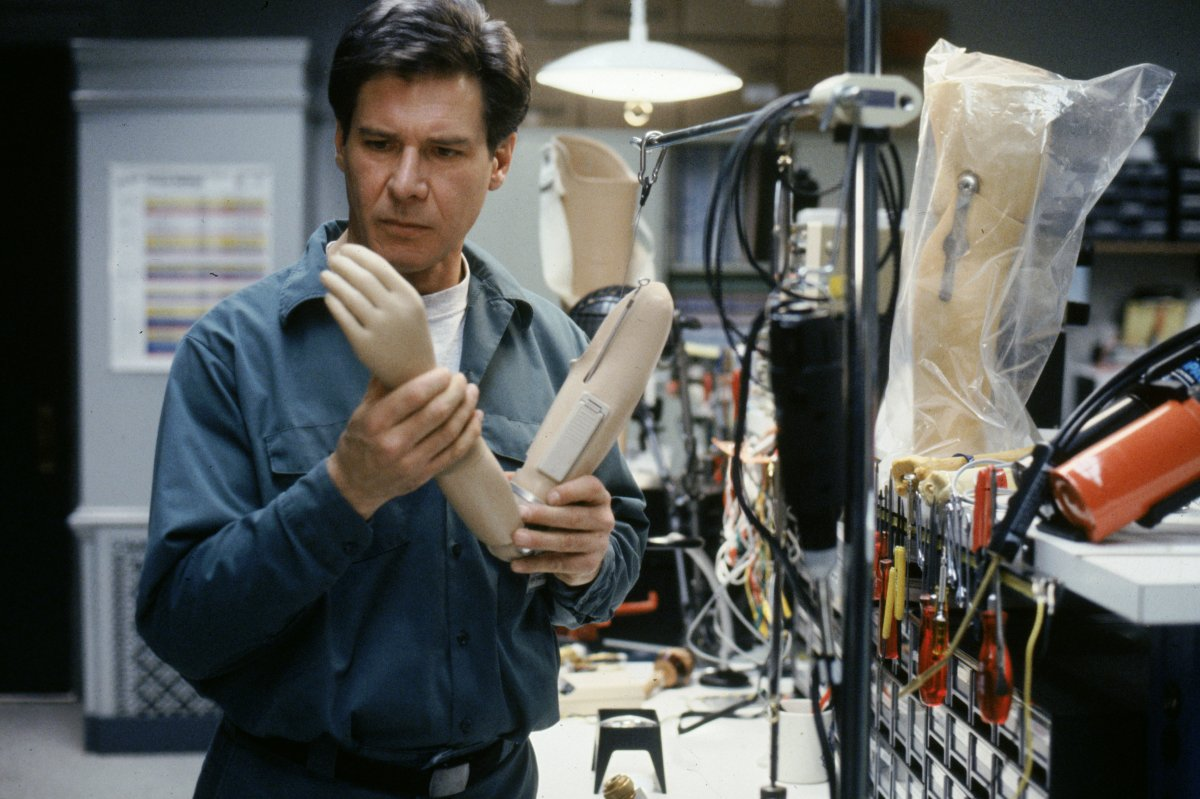
\includegraphics[width=.5\linewidth]{img/thefugitive} 

}

\caption{Harrison Ford's character on the hunt for the one-armed man who killed his wife. Image Source: http://www.imdb.com/title/tt0106977/}\label{fig:fugitive}
\end{figure}

\subsection{Strength of Evidence: Discrete
Data}\label{strength-of-evidence-discrete-data}

For discrete data like blood type and DNA, when we want to find the
probability of a match by chance, there are several important
considerations:

\begin{enumerate}
\def\labelenumi{\arabic{enumi}.}
\tightlist
\item
  This evidence is usually \_\_\_\_\_\_\_\_\_\_\_\_\_ centered: material
  from scene is considered \_\_\_\_\_\_\_\_\_ and we want to compute the
  likelihood that an individual would have a similar
  object/characteristic. \vspace{.1in}
\item
  This evidence depends on relevant ``\_\_\_\_\_\_\_\_\_\_\_''. For
  instance, the suspect is male, the suspect is Chinese, etc.
  \vspace{.1in}
\item
  We have to consider \emph{where} our data come from. This could be
  from population records or convenience samples.
\end{enumerate}

These concerns are equally relevant to the likelihood ratio approach so
we don't discuss them further here. See \ref{likelihood-ratio} for more.

\subsection{Strength of Evidence: Continuous
Data}\label{strength-of-evidence-continuous-data}

For continuous data, finding the probability of a match by chance is
typically a bit harder to do. We need the likelihood that objects
(e.g.~glass fragments) selected at random would match crime scene
sample. The basic idea is outlined below, using terms from the
\(t\)-test context. (See Section \ref{normal-data} for reference.)

\begin{enumerate}
\def\labelenumi{\arabic{enumi}.}
\tightlist
\item
  Suppose for the moment we know the ``population'' mean of a randomly
  chosen glass source.
\item
  We can find the probability that a \(t\)-test based on a sample from
  this \emph{random} object will result in agreement with the
  \emph{crime scene} sample.
\item
  The total coincidental agreement probability is an average over
  \emph{all possible choices} for the random source:
  \[ \text{coincidence probability} = \sum\limits_{\text{pop. means}} Pr(\text{a mean}) Pr(\text{match to scene sample} | \text{a mean})\]
\end{enumerate}

This procedure is technically challenging but it can be done! The key
question is: Where does the information about the set of possible random
sources (i.e.~the relevant population) come from?

\subsubsection{Example}\label{example-2}

Let's illustrate this idea with an example. Consider again the data from
Curran et al. (\protect\hyperlink{ref-curranetal}{1997}). Recall the
crime scene example, call it \(X\), has 5 observations with a mean
aluminum concentration of \(\overline{X} = 0.730\) and standard
deviation of \(0.04\).

Assume we will apply a standard statistical test with 5 samples from an
unknown randomly chosen glass source, with a cutoff corresponding to a
\(p\)-value of 0.05. So, we will only reject the null hypothesis (that
the random sample comes from the same source as the crime scene sample)
if the test statistic is so large that it has a less than 5\% chance of
occurring at random. Any value that falls in the 95\% non-rejection
range will be deemed ``indistinguishable'' from the crime scene sample.

Next, suppose that the means of \emph{all} randomly chosen glass sources
from the population of interest can be descried using a normal
distribution with mean \(\mu = 0.83\) and standard deviation
\(\sigma = 0.10\). This distribution is shown in Figure
\ref{fig:normglass}. In the population of glass sources, some randomly
chosen sources will have means near 0.73 and will be \_\_\_\_\_\_\_\_ to
distinguish from the control sample. Some randomly chosen sources will
have means near 0.83 and will likely be \_\_\_\_\_\_\_\_\_\_\_\_\_ from
the control sample. Some randomly chosen sources will have means near
.93 and will be \_\_\_\_\_\_\_\_ to distinguish from the control sample.

Under this setup, we can compute how likely it is to find a randomly
chosen source which provides a sample that is indistinguishable from the
crime scene sample. The answer is 0.24 or 24\% of the time

\begin{figure}[h]

{\centering 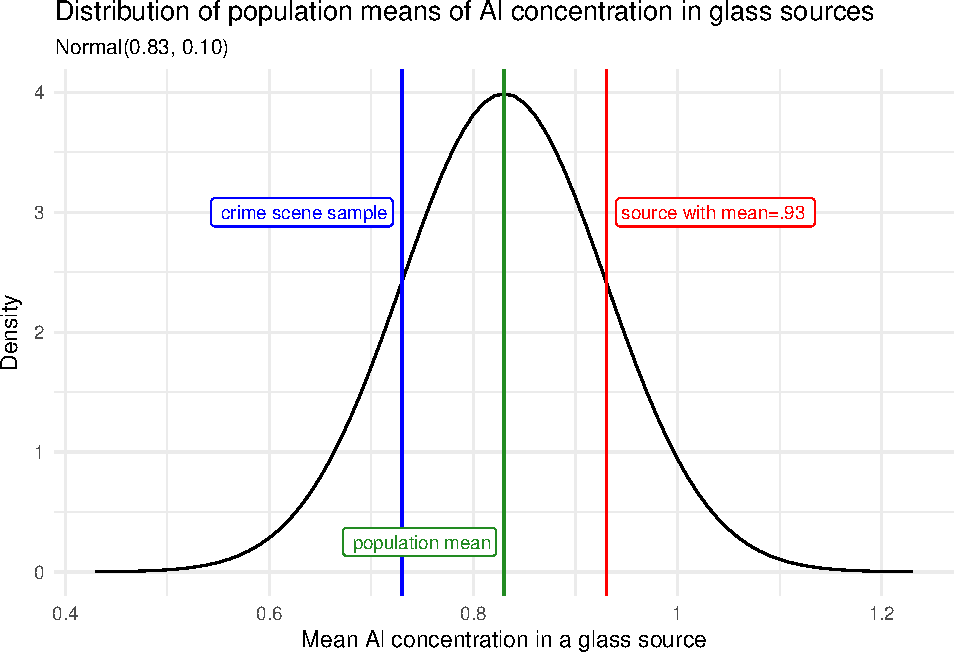
\includegraphics[width=.5\linewidth]{STfFP-Workbook_files/figure-latex/normglass-1} 

}

\caption{The population distribution of mean aluminum concentrations in all randomly chosen glass sources.}\label{fig:normglass}
\end{figure}

We can repeat the same idea for finding coincidence probabilities for
different population means and standard deviations. The table shown
below gives the different coincidence probabilities (cp) for different
population means and standard deviations.

\begin{longtable}[]{@{}ccc@{}}
\caption{Coincidence probabilities for different population
distributions.}\tabularnewline
\toprule
\begin{minipage}[b]{0.09\columnwidth}\centering\strut
mean\strut
\end{minipage} & \begin{minipage}[b]{0.06\columnwidth}\centering\strut
sd\strut
\end{minipage} & \begin{minipage}[b]{0.06\columnwidth}\centering\strut
cp\strut
\end{minipage}\tabularnewline
\midrule
\endfirsthead
\toprule
\begin{minipage}[b]{0.09\columnwidth}\centering\strut
mean\strut
\end{minipage} & \begin{minipage}[b]{0.06\columnwidth}\centering\strut
sd\strut
\end{minipage} & \begin{minipage}[b]{0.06\columnwidth}\centering\strut
cp\strut
\end{minipage}\tabularnewline
\midrule
\endhead
\begin{minipage}[t]{0.09\columnwidth}\centering\strut
0.73\strut
\end{minipage} & \begin{minipage}[t]{0.06\columnwidth}\centering\strut
0.2\strut
\end{minipage} & \begin{minipage}[t]{0.06\columnwidth}\centering\strut
0.2\strut
\end{minipage}\tabularnewline
\begin{minipage}[t]{0.09\columnwidth}\centering\strut
0.83\strut
\end{minipage} & \begin{minipage}[t]{0.06\columnwidth}\centering\strut
0.2\strut
\end{minipage} & \begin{minipage}[t]{0.06\columnwidth}\centering\strut
0.37\strut
\end{minipage}\tabularnewline
\begin{minipage}[t]{0.09\columnwidth}\centering\strut
0.93\strut
\end{minipage} & \begin{minipage}[t]{0.06\columnwidth}\centering\strut
0.2\strut
\end{minipage} & \begin{minipage}[t]{0.06\columnwidth}\centering\strut
0.65\strut
\end{minipage}\tabularnewline
\begin{minipage}[t]{0.09\columnwidth}\centering\strut
0.73\strut
\end{minipage} & \begin{minipage}[t]{0.06\columnwidth}\centering\strut
0.1\strut
\end{minipage} & \begin{minipage}[t]{0.06\columnwidth}\centering\strut
0.37\strut
\end{minipage}\tabularnewline
\begin{minipage}[t]{0.09\columnwidth}\centering\strut
0.83\strut
\end{minipage} & \begin{minipage}[t]{0.06\columnwidth}\centering\strut
0.1\strut
\end{minipage} & \begin{minipage}[t]{0.06\columnwidth}\centering\strut
0.24\strut
\end{minipage}\tabularnewline
\begin{minipage}[t]{0.09\columnwidth}\centering\strut
0.93\strut
\end{minipage} & \begin{minipage}[t]{0.06\columnwidth}\centering\strut
0.1\strut
\end{minipage} & \begin{minipage}[t]{0.06\columnwidth}\centering\strut
0.17\strut
\end{minipage}\tabularnewline
\begin{minipage}[t]{0.09\columnwidth}\centering\strut
0.73\strut
\end{minipage} & \begin{minipage}[t]{0.06\columnwidth}\centering\strut
0.05\strut
\end{minipage} & \begin{minipage}[t]{0.06\columnwidth}\centering\strut
0.12\strut
\end{minipage}\tabularnewline
\begin{minipage}[t]{0.09\columnwidth}\centering\strut
0.83\strut
\end{minipage} & \begin{minipage}[t]{0.06\columnwidth}\centering\strut
0.05\strut
\end{minipage} & \begin{minipage}[t]{0.06\columnwidth}\centering\strut
0.06\strut
\end{minipage}\tabularnewline
\begin{minipage}[t]{0.09\columnwidth}\centering\strut
0.93\strut
\end{minipage} & \begin{minipage}[t]{0.06\columnwidth}\centering\strut
0.05\strut
\end{minipage} & \begin{minipage}[t]{0.06\columnwidth}\centering\strut
0.002\strut
\end{minipage}\tabularnewline
\bottomrule
\end{longtable}

The moral of the story, is that the probability of a coincidental match
is high when there is\ldots{}

\begin{itemize}
\tightlist
\item
  a small difference between control sample and the population of
  randomly chosen sources (i.e.~the crime scene/control sample is
  ``ordinary'').
\item
  a large amount of heterogeneity among the potential sources in the
  population.
\item
  a large amount of variability among the fragments in an individual
  source.
\end{itemize}

\subsection{Likelihood Ratio}\label{likelihood-ratio}

The goal for the \_\_\_\_\_\_ of \_\_\_\_\_\_\_ in a courtroom setting
is to make a decision about the relative likelihood of two hypotheses
(e.g.~same source or different source) \emph{given} the data. In
statistical terms, this is a \textbf{Bayesian formulation} because we
ask for probabilities about the state of the world \emph{given} observed
data. Recall from Section \ref{bayes-rule} Bayes' Rule (or Bayes'
Theorem): given two events A and B we have the probability of A
\emph{given} B:

\[P(A|B) = \frac{P(A)P(B|A)}{P(B)}\] \clearpage 

Bayes' rule is a way of \_\_\_\_\_\_\_\_\_\_ the direction of
conditional probabilities. We can go from statements about the
likelihood of the \textbf{evidence} given the \_\_\_\_\_\_\_\_\_\_\_ to
statements about the likelihood of the \textbf{hypotheses} given the
\_\_\_\_\_\_\_\_\_\_\_.

Formally, for the evidence (\(E\)) and having same source (\(S\)), we
write:

\[P(S|E) = \frac{P(E|S)P(S)}{P(E|S)P(S) + P(E|\overline{S})P(\overline{S})}.\]

Recall from Section \ref{bayes-rule-to-the-likelihood-ratio} that Bayes'
Rule can be rewritten in terms of the odds in favor of the same source
hypothesis (left-hand side of the equation):

\[\frac{P(S|E)}{P(\overline{S}|E)} = \frac{P(E|S)}{P(E|\overline{S})}\frac{P(S)}{P(\overline{S})}\]

In words, we can describe the above equation as ``the posterior odds of
the same source hypothesis is equal to the likelihood ratio of the
evidence times the prior odd of the same source hypothesis.'' The
\emph{likelihood ratio} (sometimes called the Bayes Factor) is a measure
of the value of the evidence. It does \emph{not} depend on the prior
beliefs with regards to the same source hypothesis.

\begin{equation}\label{eq:lr}
LR = \frac{P(E|S)}{P(E|\overline{S})}
\end{equation}

The term ``likelihood'' is used because if \(E\) includes continuous
measurements, then we cannot talk about probability of single events.
The likelihood ratio could, in principle, be used with \(E\)
representing ``all'' evidence of all types (more on this later). In
addition, other available information (e.g.~background) can be
incorporated into the LR (more on this later as well).

The \textbf{interpretation} of the likelihood ratio is crucial. The
derivation of the LR (see \ref{eq:7}) shows that the LR is a factor that
we should use to change our same source odds. Furthermore, there are
some proposals for scales (e.g.~ENFSI) that map LRs to words:

\begin{itemize}
\tightlist
\item
  LR from 2-10 implies \_\_\_\_\_ support of the same source
  hypothesis\vspace{.1in}
\item
  LR from 10-100 implies \_\_\_\_\_\_\_\_ support of the same source
  hypothesis\vspace{.1in}
\item
  See page 17 of
  \url{http://enfsi.eu/wp-content/uploads/2016/09/m1_guideline.pdf} for
  the complete scale from ENFSI (European Network of Forensic Science
  Institutes)
\end{itemize}

There is some confusion about terminology. To clear this up, it is
important to understand how the LR approach and the Bayesian approach
relate. The LR (often called the Bayes Factor) plays a central role in a
Bayesian approach to forensic evidence: it is the quantity used to
update \emph{a priori} odds in order to obtain posterior odds. The true
distinction between the LR and the Bayes factor is technical and has to
do with how statistical parameters are treated.

Let's return to Equation \ref{eq:lr}. The numerator, \(P(E|S)\) assumes
\_\_\_\_\_\_\_\_\_ source and asks about the likelihood of the evidence
in that case. This value is somewhat related to finding a \(p\)-value
for testing the hypothesis of equal means but, there is no binary
decision regarding a match in the LR approach. Instead, think of the LR
as a quantitative measure of likelihood of evidence under the same
source hypothesis, \(S\). The denominator, \(P(E|\overline{S})\),
assumes no \_\_\_\_\_\_\_\_ \_\_\_\_\_\_\_ and asks about the likelihood
of the evidence in that case. This is analogous to finding coincidence
probability like we did in Section
\ref{strength-of-evidence-continuous-data}. Here too, as in the
numerator, we do not require a binary decision regarding a match. The
denominator is a quantitative measure of likelihood of evidence under
\_\_\_\_\_\_.

The LR approach makes explicit the need to consider the evidence under
\_\_\_\_\_ different hypotheses. It also separates
``\_\_\_\_\_\_\_\_\_\_\_\_'' information about evidence from
``\_\_\_\_\_\_\_\_\_\_\_'' assessments of the same source hypothesis
\(S\). There is some subtlety here. Do not fall prey to the\ldots{}

\begin{itemize}
\tightlist
\item
  Prosecutor's \_\_\_\_\_\_\_\_\_: interpreting \(P(E|\overline{S})\) as
  \(P(\overline{S}|E)\). i.e.~if evidence is unlikely under
  \(\overline{S}\) that fact is mistakenly interpreted as saying that
  \(\overline{S}\) is unlikely. \vspace{.1in}
\item
  \_\_\_\_\_\_\_\_\_\_\_\_ attorney's fallacy: other misinterpretations
  of \(P(E|\overline{S})\), such as if
  \(P(E|\overline{S}) = \frac{1}{1,000,000}\), then there are 300 other
  people in the U.S. who could have been the source (and thus committed
  the crime).
\end{itemize}

Let's define \(E=(x,y)\), where \(y\) represents the measurement of
evidence from the crime scene, and \(x\) represents the measurement of
evidence from the suspect. Then, we can rewrite the likelihood ratio
using laws of probability from Section \ref{conditional-probability}:

\begin{equation}\label{eq:lrredo}
\begin{split}
LR & = \frac{P(E|S)}{P(E|\overline{S})} \\
  & = \frac{p(x,y | S)}{p(x,y | \overline{S}} \\ 
  & = \frac{p(y | x, S)}{p(y | x, \overline{S}} \cdot \frac{p(x| S)}{p(x| \overline{S}} 
\end{split}
\end{equation}

Often, the likelihood of \(x\) is the same for \_\_\_\_\_\_ and
\_\_\_\_\_\_, i.e. \(p(x| S)= p(x| \overline{S})\). In other words, the
distribution of the suspect's data does not depend on who committed the
crime. This leads to yet another way to write the likelihood ratio:

\begin{equation}\label{eq:lr3}
LR = \frac{p(y | x, S)}{p(y | x, \overline{S}}
\end{equation}

So, the likelihood ratio is the ratio of the probability of finding the
evidence at the crime scene \emph{given} the evidence from the suspect
\textbf{and} the same source assumption, to the probability of finding
the evidence at the crime scene \emph{given} the evidence from the
suspect \textbf{and} the different source assumption.

Let's assume we start with Equation \ref{eq:lr3}:

\begin{itemize}
\tightlist
\item
  In the \_\_\_\_\_\_\_\_\_\_\_ case, the numerator (probability of
  finding the evidence at the crime scene \emph{given} the evidence from
  the suspect \textbf{and} the same source assumption) is typically 0 or
  1, or values really close to those. (We should also consider the
  possibility of a lab error or contamination.) The denominator
  (probability of finding the evidence at the crime scene \emph{given}
  the evidence from the suspect \textbf{and} the different source
  assumption) is then the probability of a \_\_\_\_\_\_\_\_\_\_\_\_\_
  match. \vspace{.1in}
\item
  In the \_\_\_\_\_\_\_\_\_\_\_\_\_ case, the numerator is a measure of
  how likely it is to observe the numbers \((x,y)\) if they represent
  multiple measures from the same source. The denominator is a measure
  of how likely it is to observe the numbers \((x,y)\) if they are
  measures from two different sources.
\end{itemize}

\subsubsection{Example}\label{example-3}

Suppose the evidence is the blood type for a crime scene sample and the
blood type for a suspect sample. We have information about the
distribution of blood types in the population:

\begin{tabular}{l|cccc}
Type & A & B & AB & O \\
U.S. frequency & 0.42 & 0.10 & 0.04 & 0.44
\end{tabular}

Suppose both samples are observed to be of blood type O. Then,
\(Pr(y = O|x = O,S) \approx 1\). We'd expect to see the same blood type
if the samples come from the same source. Conversely,
\(Pr(y = O|x = O,\overline{S}) = 0.44\). Blood type O is fairly common
in the U.S. So the LR is \(LR \approx \frac{1}{0.44} \approx 2.27\).
Following the ENFSI language, the evidence provides \_\_\_\_\_\_\_
support for the ``same source'' hypothesis. Blood type AB, however, is
rare in the U.S. If the two samples were both AB, then LR would indicate
stronger evidence (LR would be \(\approx \frac{1}{.04} \approx 25\)).

\subsubsection{Where it works: DNA}\label{where-it-works-dna}

A DNA profile identifies alleles at a number of different locations
along the genome. For example, alleles at location TH01 are 7,9. As with
blood type, we may see matching profiles from the crime scene and from
the suspect. The numerator is also approximately one as in blood type
example because we expect DNA samples from the same source to be
indistinguishable. We can the determine the probability of a
coincidental match for each marker or location:

\begin{tabular}{lccccccccc}
TH01 & 4 & 5 & 6 & 7 & 8 & 9 & 9.3 & 10 & 11 \\ 
Freq. & 0.001 & 0.001 & 0.266 & 0.160 & 0.135 & 0.199 & 0.200  & 0.038 & 0.001
\end{tabular}

For TH01 agreeing on alleles 7, 9, the probability of a random agreement
is 2\emph{.16}.199 = .064. Thus, the LR in this case is
\(\frac{1}{0.064} \approx 15\).

DNA evidence consists of data for a number of locations (CODIS used 13
locations pre-2017). The locations on different chromosomes are
independent. Recall that if events are independent, then we can multiply
probabilities (which basically means multiplying likelihood ratios). So,
a match at \emph{all} locations can lead to likelihood ratios in the
\textbf{billions} (or even larger).

The likelihood ratio approach works well for DNA because the underlying
biology is well understood. The probability model for the evidence
follows directly from genetic theory, and population databases are
available for computing random match probabilities. In addition, for
single-source DNA sample, the methodology has been peer--reviewed and is
well accepted by the scientific community. But, even with the above
information, there are still problems arising in the DNA forensic field.
For example, allele calling still has some subjective elements despite
the reputation of pure objectivity, and DNA samples containing multiple
sources (i.e.~DNA mixtures) still are not as well-understood as
single-source samples.

\subsubsection{Where it can work: Trace
evidence}\label{where-it-can-work-trace-evidence}

Glass and bullet lead are examples of where the likelihood ratio
approach can potentially work. We can measure chemical concentrations of
elements in glass (or bullet lead). There may be broken glass at the
crime scene and glass fragments on a suspect. But can we construct a
likelihood ratio for evidence of this type? Perhaps\ldots{} We can
motivate this with some pictures from elemental analyses of bullet lead
(see Figure \ref{fig:projs}) and refractive indices of glass (see Figure
\ref{fig:wibw}).

\begin{figure}
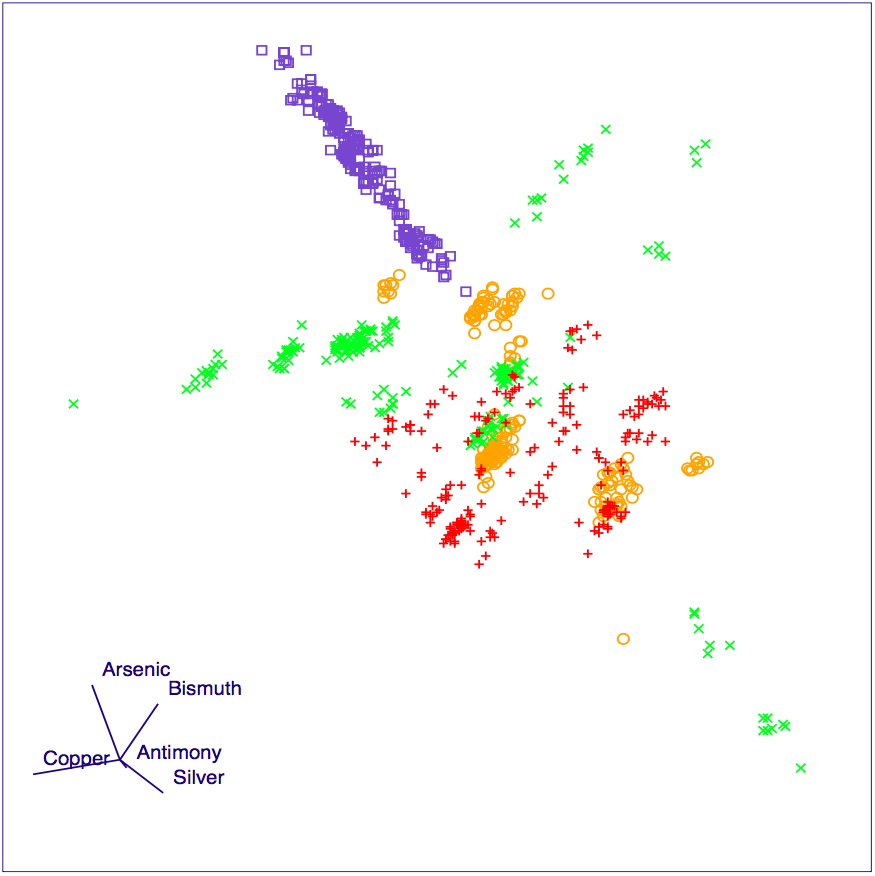
\includegraphics[width=0.32\linewidth]{img/proj1} 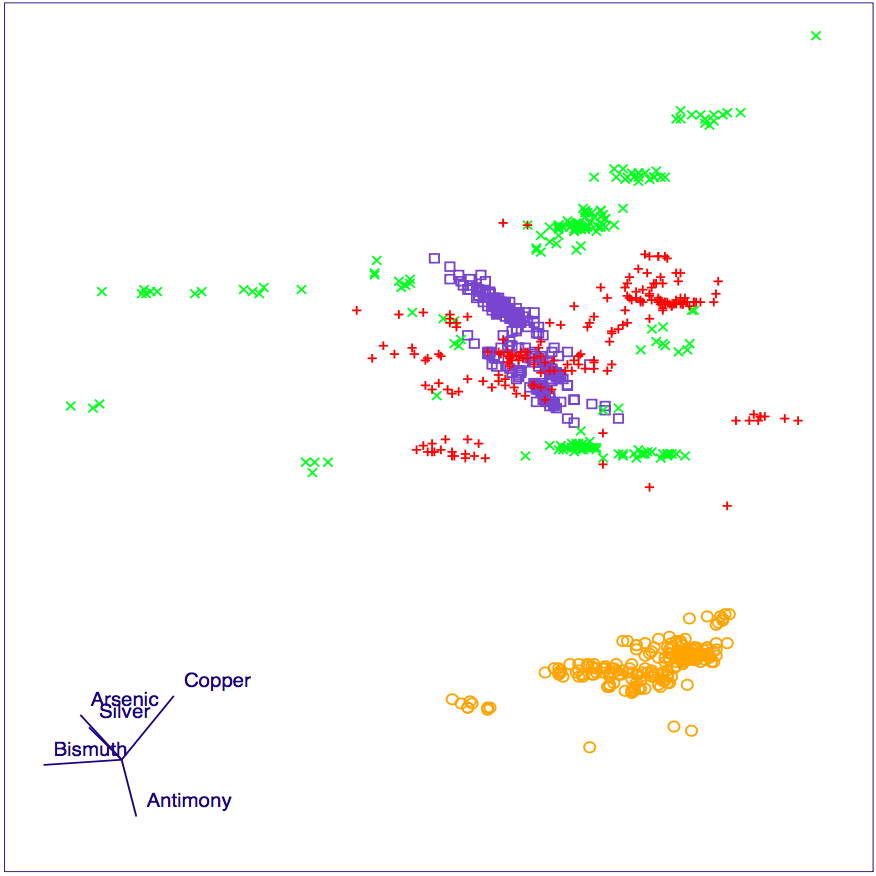
\includegraphics[width=0.32\linewidth]{img/proj2} 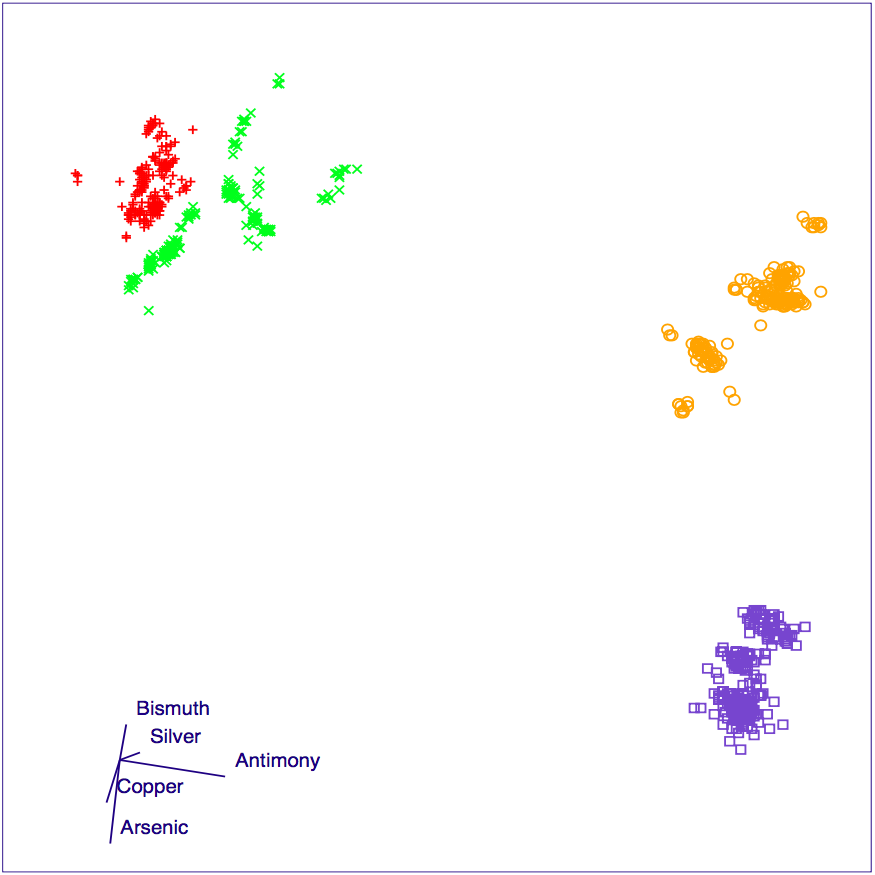
\includegraphics[width=0.32\linewidth]{img/proj3} \caption{Three projections of 5-dimensional bullet lead trace element data.}\label{fig:projs}
\end{figure}

\begin{figure}
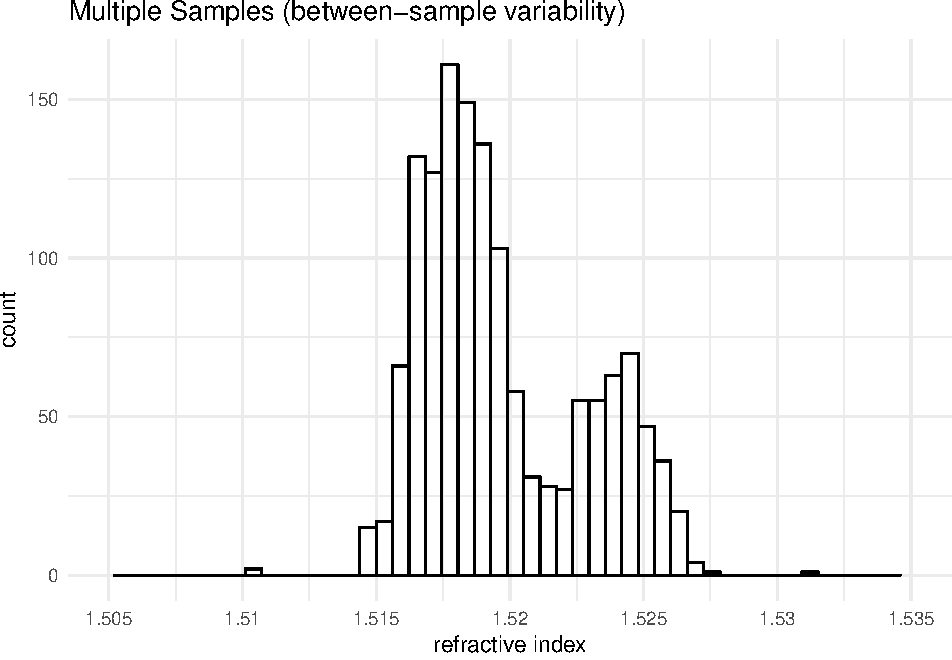
\includegraphics[width=0.32\linewidth]{STfFP-Workbook_files/figure-latex/wibw-1} 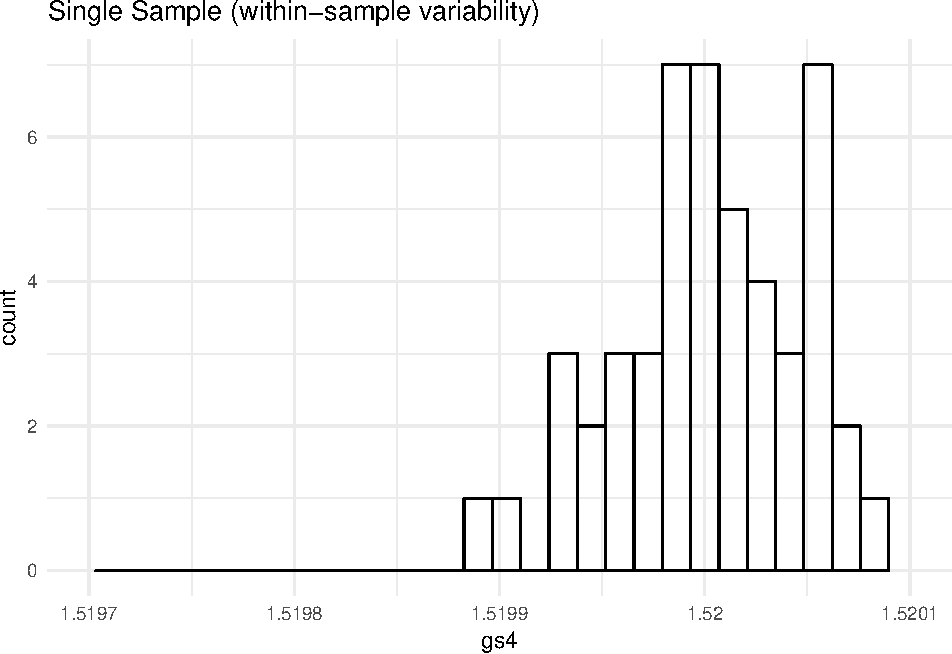
\includegraphics[width=0.32\linewidth]{STfFP-Workbook_files/figure-latex/wibw-2} 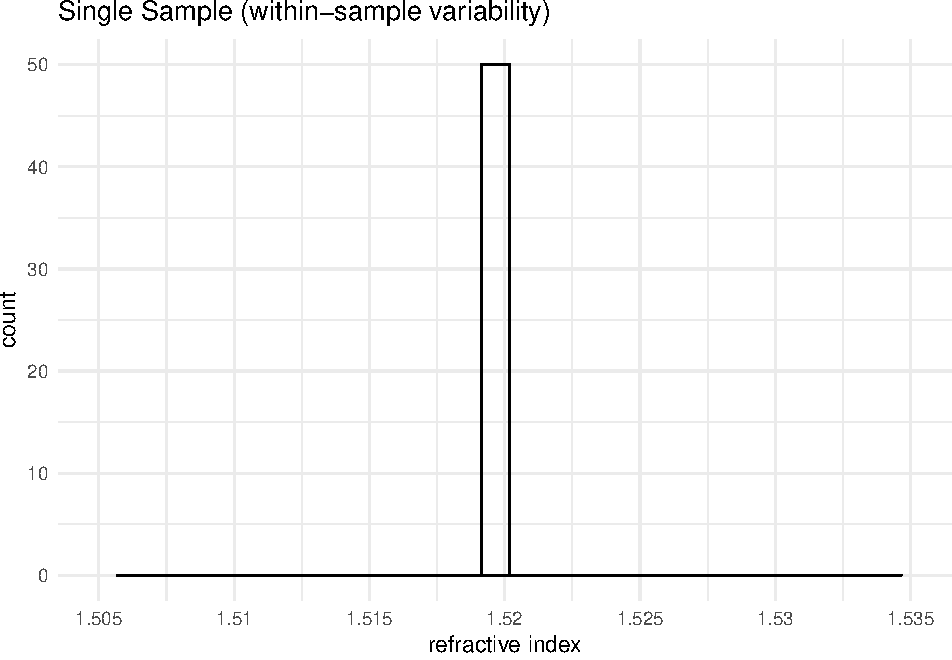
\includegraphics[width=0.32\linewidth]{STfFP-Workbook_files/figure-latex/wibw-3} \caption{From left to right: multiple glass source samples where refractive index was reported, the same measurements for just one of those sources, and the data from the middle source on the same $x$ axis as all three sources.}\label{fig:wibw}
\end{figure}

A conceptual discussion of the likelihood ratio approach is described by
Aitken and Lucy (\protect\hyperlink{ref-aitkenlucy}{2004}). They take
\(y\) and \(x\) to be trace element concentrations for a single element
(or multiple elements) from several glass fragments at the scene (\(y\))
and on the subject (\(x\)). Then, they assume a normal distribution for
trace element concentrations, though this assumption may be more
reasonable for the natural log values of the concentrations. In this
setup, under the same source hypothesis \(S\), \(x\) and \(y\) are two
sets of measurements from a single source (i.e.~from a single normal
distribution). But, under the different source hypothesis,
\(\overline{S}\), \(x\) and \(y\) are sets of measurements from two
different sources (i.e.~from two different normal distributions drawn
from the relevant population of possible sources).

It is then possible compute a likelihood ratio in this scenario if we
have information about:

\begin{enumerate}
\def\labelenumi{\arabic{enumi}.}
\tightlist
\item
  The \_\_\_\_\_\_\_\_\_ of repeated measurements from a
  \_\_\_\_\_\_\_\_\_ source. \vspace{.1in}
\item
  The variability among \_\_\_\_\_\_ measurements from
  \_\_\_\_\_\_\_\_\_\_ sources in the population of
  interest.\vspace{.1in}
\item
  The average or typical measurement for random sources in the
  population of interest.
\end{enumerate}

Aitken and Lucy's key findings were:

\begin{enumerate}
\def\labelenumi{\arabic{enumi}.}
\tightlist
\item
  LR is small if \(y\) and \(x\) are very different (i.e.~different
  source hypothesis)
\item
  LR is big if \(y\) and \(x\) are similar and \(y\) is unusual for the
  population of interest (i.e.~they are indistinguishable on an unusual
  value)
\item
  Their examples find typical LRs in 100s or 1000s.
\item
  Aitken and Lucy also show how to take the likelihood ratio approach
  without the strong normal (or lognormal) distribution assumptions.
\end{enumerate}

In conclusion, the LR approach can work for trace evidence when

\begin{enumerate}
\def\labelenumi{\arabic{enumi}.}
\tightlist
\item
  there is a well-defined set of \_\_\_\_\_\_\_\_\_\_\_ (e.g.~chemical
  concentrations)\vspace{.1in}
\item
  there is plausible probability models to describe
  \_\_\_\_\_\_\_\_\_\_\_\_ within a sample (e.g.~normal distribution or
  less restrictive models)\vspace{.1in}
\item
  it is possible to sample from a population (e.g.~other windows) to
  assess variation across different sources.
\end{enumerate}

This can be and has been done:

\begin{itemize}
\tightlist
\item
  In Aitken and Lucy (\protect\hyperlink{ref-aitkenlucy}{2004}) with
  glass
\item
  In Carriquiry, Daniels, and Stern
  (\protect\hyperlink{ref-aliciaetal}{2000}) et al with bullet lead
\end{itemize}

But, likelihood ratios can be very sensitive to assumptions that are
made, and assessing the relevant ``population'' is hard, and may vary
from case to case.

\subsubsection{Where it might work: Pattern
evidence}\label{where-it-might-work-pattern-evidence}

Many forensic disciplines are focused on comparing a sample, or
\_\_\_\_\_\_\_\_\_, at the crime scene (the ``unknown'' or
``\_\_\_\_\_\_\_\_\_\_\_\_'') and a potential source (the ``known'').
The goal is to assess whether two samples have the \_\_\_\_\_\_\_\_\_\_
source or two different sources. There are many examples of trace
evidence in forensic science (See Figure \ref{fig:trace}):

\begin{itemize}
\tightlist
\item
  Latent print examinations\footnote{Image source:
    \url{http://science.sciencemag.org/content/309/5736/892/F4}}
\item
  Shoe prints\footnote{Image source: Smith
    (\protect\hyperlink{ref-shoepic}{2009})}
\item
  Tire tracks
\item
  Questioned documents\footnote{Image source:
    \url{http://forensicunit.weebly.com/evidence.html}}
\item
  Firearms
\item
  Tool marks
\end{itemize}

\begin{figure}
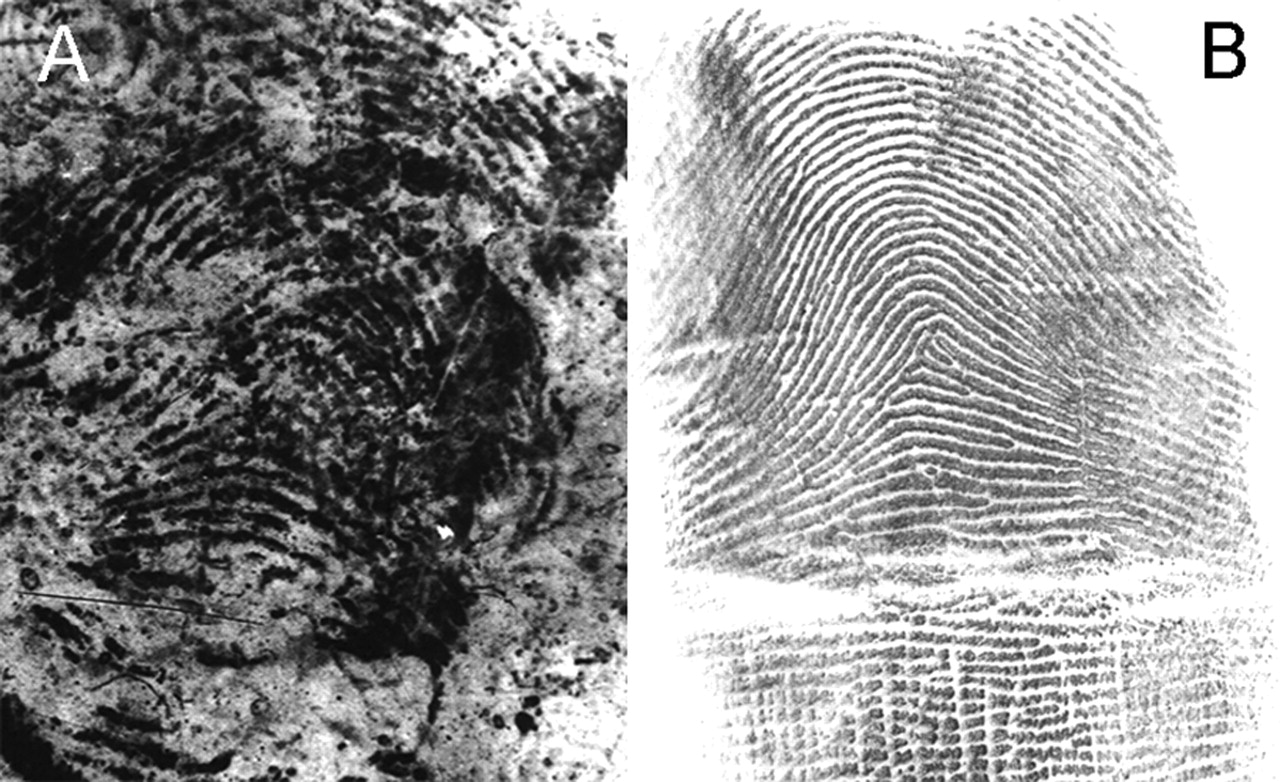
\includegraphics[width=0.32\linewidth]{img/mayfieldfinger} 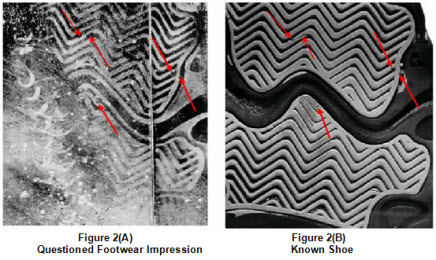
\includegraphics[width=0.32\linewidth]{img/shoecompare} 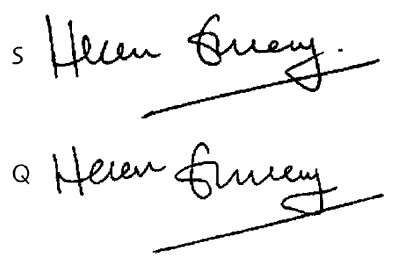
\includegraphics[width=0.32\linewidth]{img/signature} \caption{Examples of pattern evidence comparisons where there is potential application of the likelihood ratio approach for source determination. From left to right: latent print, shoe print, and questioned signature comparisons.}\label{fig:trace}
\end{figure}

There are a number of challenges in constructing likelihood ratios for
pattern evidence:

\begin{enumerate}
\def\labelenumi{\arabic{enumi}.}
\tightlist
\item
  The data are very \_\_\_\_\_\_ \_\_\_\_\_\_\_\_\_ (often are images).
  \vspace{.1in}
\item
  There is a great deal of flexibility (subjectivity?) in defining the
  numbers or types of \_\_\_\_\_\_\_\_\_\_ to look at. \vspace{.1in}
\item
  There is a lack of probability models for \_\_\_\_\_\_\_\_\_\_\_\_\_
  features or patters. \vspace{.1in}
\item
  There is still a need to study \_\_\_\_\_\_\_\_\_\_\_ across a
  relevant population.
\end{enumerate}

These challenges are very hard overcome, but there is work underway,
including at CSAFE institutions, to create the necessary statistical
foundations for pattern evidence.

Consider the latent fingerprint example in Figure \ref{fig:finger} from
Neumann et al. (\protect\hyperlink{ref-neumann15}{2015}). In the
authors' approach, each minutiae is characterized by direction/angle,
type of minutiae, and shape/configuration. Neumann et al compute
separate likelihood ratios for each of these characteristics, where the
\_\_\_\_\_\_\_\_\_\_\_ is based on variation within the same finger
(obtained from a distortion model) and the \_\_\_\_\_\_\_\_\_\_\_\_\_\_
is based variation across different fingers (using the nearest non-match
from a database search).

\begin{figure}

{\centering 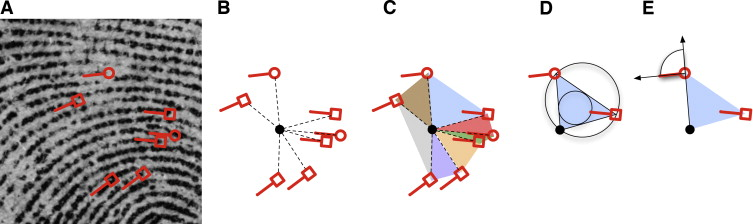
\includegraphics[width=.75\linewidth]{img/neumannfinger} 

}

\caption{'Extraction of the variables considered by the model from the raw information available on the image of a finger impression. From left to right: (a) annotation of the minutiae on the fingerprint image distinguishing ridge endings (round) and bifurcations (square); (b) definition of the centroid and organization of the minutiae with respect to the centroid; (c) creation of the triangles; (d) extraction of shape variables for one triangle and (e) extraction of the type and direction variables of the minutiae for one triangle (the variables for all triangles are similarly extracted).' (Caption from Neumann et al, p. 158)}\label{fig:finger}
\end{figure}

\subsubsection{Score-based likelihood
ratios}\label{score-based-likelihood-ratios}

Given the challenge in developing LRs for pattern evidence, there is
some interest in a \emph{score-based} approach. With this approach, we
define a \emph{score} measuring the ``\_\_\_\_\_\_\_\_\_\_\_\_'' between
the questioned and the known samples. We then obtain the
\_\_\_\_\_\_\_\_\_\_\_\_\_\_\_\_ of scores for a sample of \emph{known
matches}, and we also obtain the distribution of scores for a sample of
known \_\_\_\_\_\_\_\_\_\_\_\_\_\_. See Figure \ref{fig:score1}.

\begin{figure}

{\centering 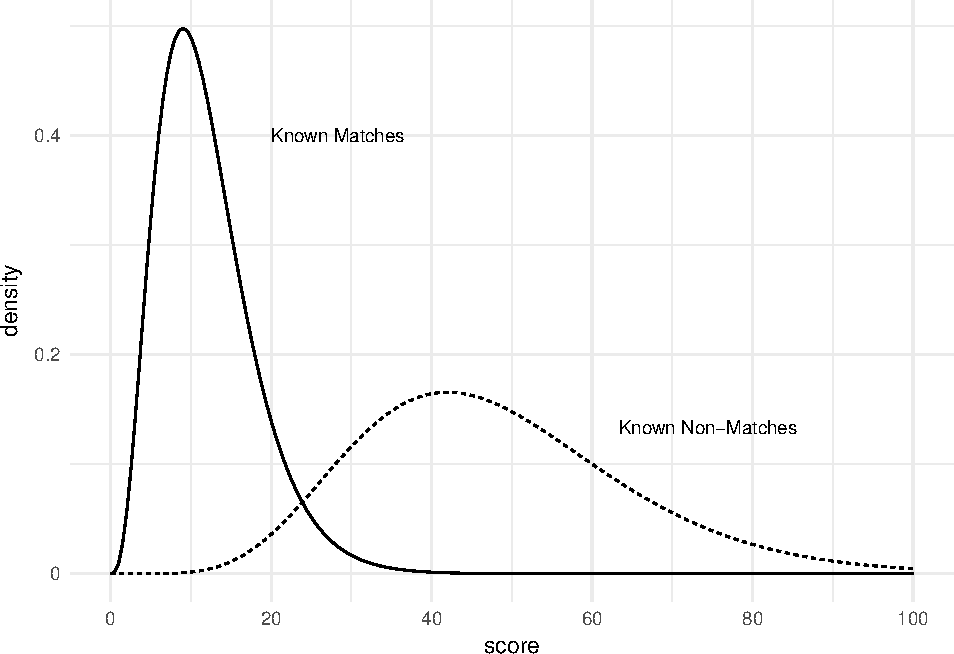
\includegraphics[width=.5\linewidth]{STfFP-Workbook_files/figure-latex/score1-1} 

}

\caption{For a sample of known matches and known non-matches, the distribution of scores for the different populations.}\label{fig:score1}
\end{figure}

The basic idea behind the score-based likelihood approach is outlined as
follows:

\begin{enumerate}
\def\labelenumi{\arabic{enumi}.}
\tightlist
\item
  Fit a probability \_\_\_\_\_\_\_\_\_\_\_\_\_\_\_\_ to the scores of
  known matches (\(Pr(S|H_p)\))\footnote{\(H_p\) is the Prosecution's
    hypothesis, that the defendant is guilty.} \vspace{.1in}
\item
  Fit a probability distribution to the scores of known nonmatches
  (\(Pr(S|H_d)\))\footnote{\(H_d\) is the Defense's hypothesis, that the
    defendant is not guilty.} \vspace{.1in}
\item
  Calculate the score-based likelihood ratio when we observe score \(S\)
  as \(SLR = \frac{Pr(S|H_p)}{Pr(S|H_d)}\). (See Figure
  \ref{fig:score2}).
\end{enumerate}

\begin{figure}

{\centering 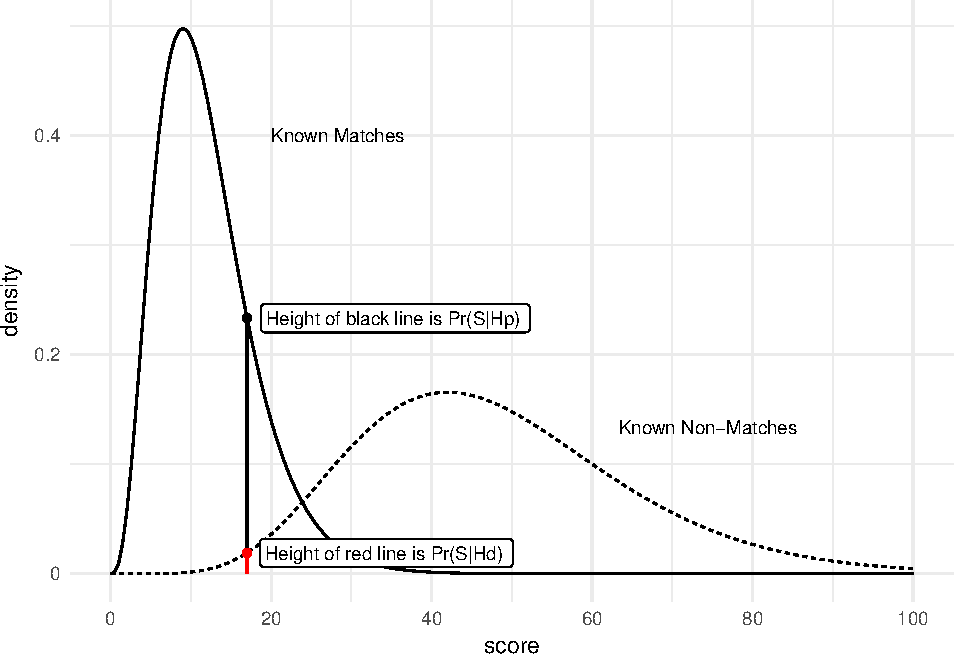
\includegraphics[width=.5\linewidth]{STfFP-Workbook_files/figure-latex/score2-1} 

}

\caption{The score distributions for known matches and known non-matches with the values in the score-based likelihood ratio calculation shown on the distributions.}\label{fig:score2}
\end{figure}

An example where the score-based likelihood approach can work for patter
evidence is with bullet land signatures, as shown by Hare, Hofmann, and
Carriquiry (\protect\hyperlink{ref-hare}{2017}). Hare et all calculated
values for many characteristics, such as the number of consecutive
matching striae and the value of the cross-correlation function, between
two bullet land comparisons. Their empirical score distributions are
shown in Figure \ref{fig:scorebullet} and an example of a comparison
they performed is shown in Figure \ref{fig:comparebullet}.

\begin{figure}

{\centering 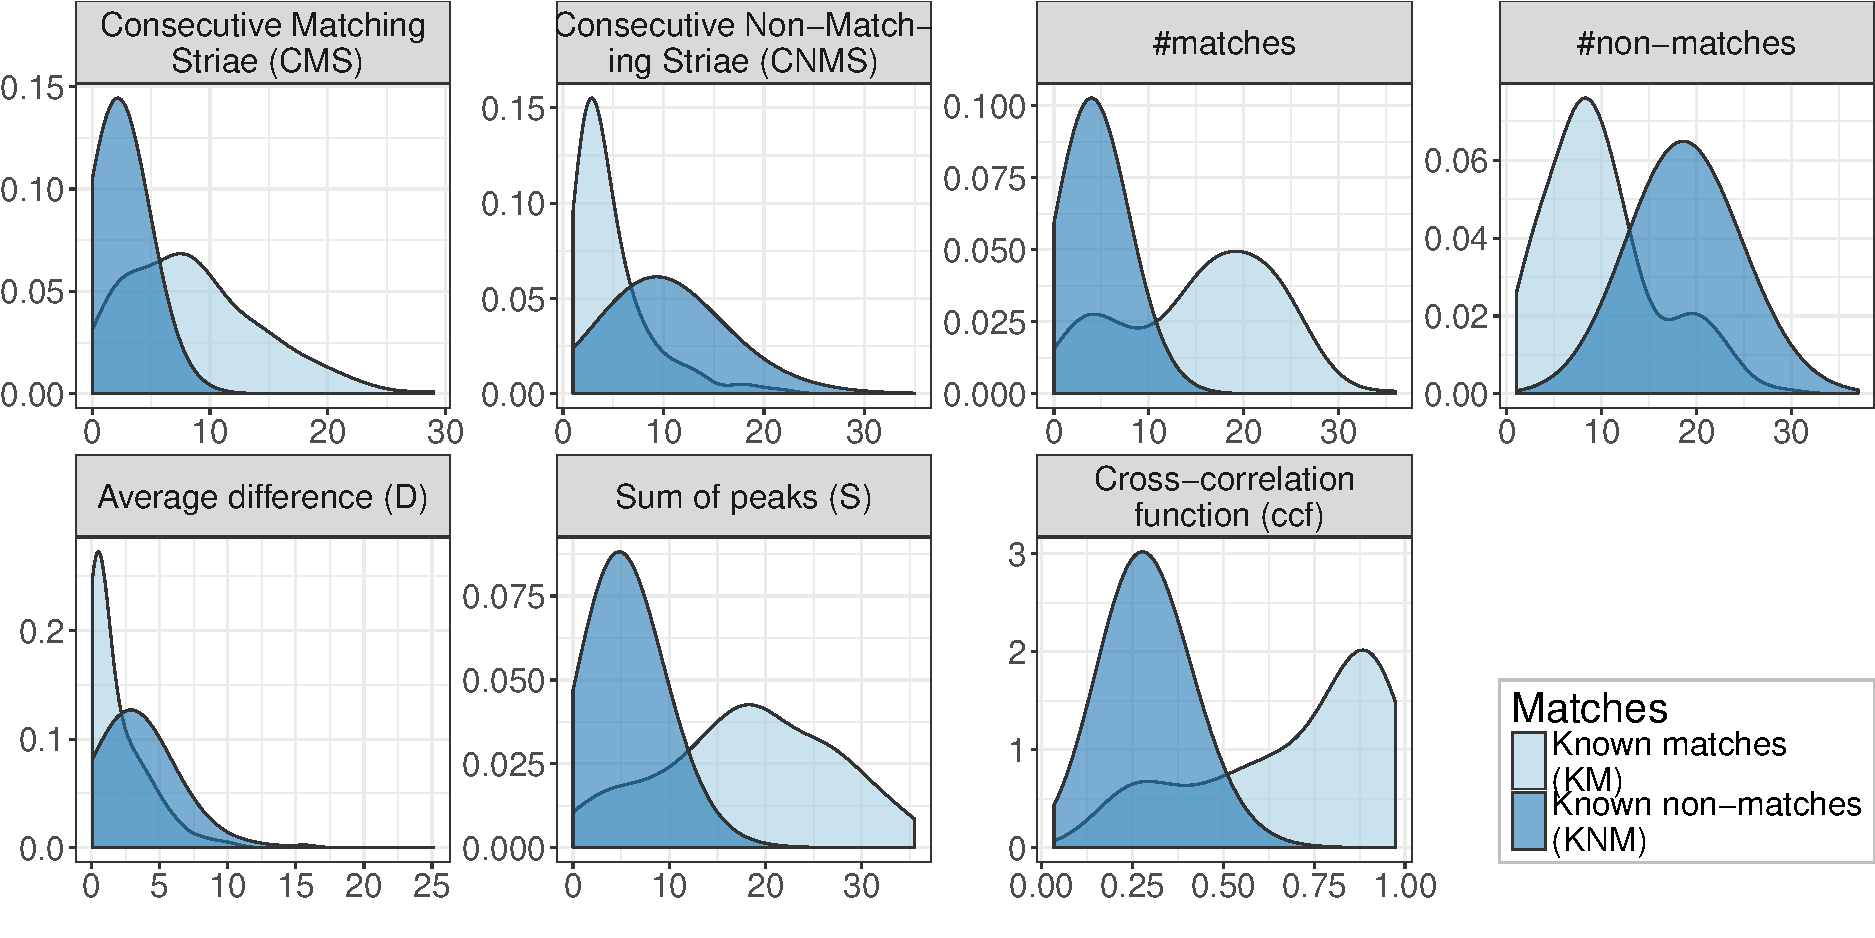
\includegraphics[width=.65\linewidth]{img/density-overview-1} 

}

\caption{Distributions of various "scores" when comparing bullet lands. Known matches in light blue, known non-matches in dark blue. Figure from Hare et al.}\label{fig:scorebullet}
\end{figure}

\begin{figure}

{\centering 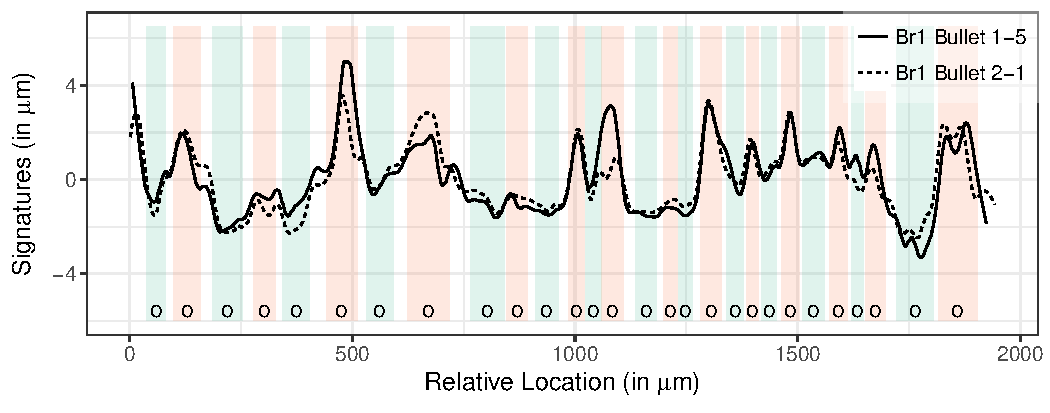
\includegraphics[width=.65\linewidth]{img/smoothmatch-1} 

}

\caption{An example of a bullet land comparison used to calculate the scores. Figure from Hare et al.}\label{fig:comparebullet}
\end{figure}

Across a number of existing examples the score distribution for known
matches seems relatively straightforward to characterize. There are,
however, challenges in defining the relevant \emph{non-match}
population:

\begin{itemize}
\tightlist
\item
  Is there a single non-match score distribution?
\item
  Should the non-match score distribution depend on characteristics of
  the crime scene sample?
\end{itemize}

Another example of score-based likelihoods comes from the Defense
Forensic Science Center's (DFSC) evaluation of a latent print score
function.\footnote{Source:
  \url{https://www.samsi.info/wp-content/uploads/2016/03/SAMSI-2016-Swofford-DFIQI-A_and_C-Combined_HJS_REVISED.ppt}}
Boxplots of score function values for known matches and non-matches by
number of minutiae matched are shown in Figure \ref{fig:minutiae}.

\begin{figure}

{\centering 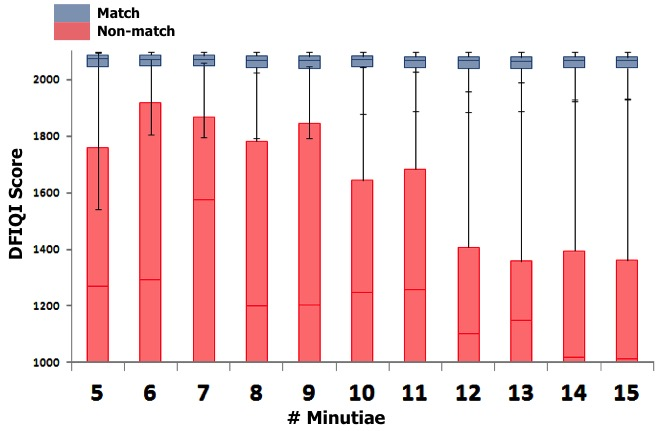
\includegraphics[width=.5\linewidth]{img/dfscscore} 

}

\caption{The score function values for known matches (blue) and known non-matches (red) by the number of matching minutiae.}\label{fig:minutiae}
\end{figure}

\subsubsection{Closing thoughts and
summary}\label{closing-thoughts-and-summary}

There is also some discussion in the community about the role of
contextual bias, task-relevant/task-irrelevant information, etc. An
advantage of the likelihood ratio framework is that it can accommodate
this discussion. Let \(E\) represent the evidence, \(S\) represent the
same source, and \(I\) represent other information that is being
considered. We can condition on this information in the LR:
\[LR = \frac{Pr(E|S,I)}{Pr(E|\overline{S},I)}\] The information \(I\)
should include task-relevant information (e.g.~substrate used), but
\(I\) should \emph{not} include results of other forensic examinations
or other case information.

In addition, the likelihood ratio can accomodate multiple types of
evidence, say \(E_1\) and \(E_2\):
\[LR = \frac{Pr(E_1,E_2|S)}{Pr(E_1, E_2|\overline{S})}\] If these
evidence types are independent, then the above expression simplifies to:
\[LR = \frac{Pr(E_1|S)}{Pr(E_1|\overline{S})}\cdot \frac{Pr(E_2|S)}{Pr(E_2|\overline{S})}\]

If the evidence types are dependent, however, determining their joint
probability (the probability of \(E_1,E_2\) occuring together) can be
incredibly difficult.

The ENFSI has released guidelines for evaluative reporting:

\begin{itemize}
\tightlist
\item
  All reporting requires:

  \begin{itemize}
  \tightlist
  \item
    \_\_\_\_\_\_\_\_\_\_\_: need to consider two propositions
    \vspace{.1in}
  \item
    \_\_\_\_\_\_\_\_\_\_\_: need to focus on the likelihood of
    \emph{evidence} given hypothesis, not the other way around
    \vspace{.1in}
  \item
    \_\_\_\_\_\_\_\_\_\_\_: should withstand scrutiny \vspace{.1in}
  \item
    \_\_\_\_\_\_\_\_\_\_\_: there should be a clear case file and report
  \end{itemize}
\item
  Concerns about the Propositions in the report:

  \begin{itemize}
  \tightlist
  \item
    Level in the hierarchy
  \item
    Absence of an alternative proposition
  \item
    Absence of specified propositions
  \item
    Changing propositions
  \end{itemize}
\item
  Assignment of the likelihood ratio:

  \begin{itemize}
  \tightlist
  \item
    data and/or expert knowledge used to assign the
    \_\_\_\_\_\_\_\_\_\_\_\_\_ required for likelihood ratio
    \vspace{.1in}
  \item
    subjective elements can be used \vspace{.1in}
  \item
    avoid undefined \_\_\_\_\_\_\_\_\_\_\_\_\_ (e.g., rare)
    \vspace{.1in}
  \item
    account for \_\_\_\_\_\_\_\_\_\_\_\_\_\_\_
  \end{itemize}
\item
  The LR then forms the basis for evaluation through verbal equivalents.
\end{itemize}

Many issues can complicate the calculation of LRs in practice. For
example:

\begin{itemize}
\tightlist
\item
  accounting for the transfer process with glass or fibers
\item
  accounting for heterogeneity due to packaging of bullets into boxes
\item
  accounting for usage/lifetime of products (e.g.~sneakers)
\end{itemize}

Though good work is being done, it seems likely that it will be some
time before LRs are available for pattern evidence. It is important to
remember that there is not one single LR for a given item of evidence.
The LR calculation depends on assumptions made and models for the
measured data and for the relevant population. Lund and Iyer (Journal of
Research of NIST, forthcoming)\footnote{\url{https://www.nist.gov/nist-research-library/journal-research-nist\#vol}}
show that the range of plausible LRs can be extremely wide!

In summary, there are some clear advantages and disadvantages to the
likelihood ratio approach. Some advantages are:

\begin{itemize}
\tightlist
\item
  Explicit comparison of the two relevant hypotheses/propositions
\item
  Provide a quantitative summary of the evidence
\item
  There is no need for arbitrary match/non-match decisions when faced
  with continuous data
\item
  It can accommodate a wide range of factors
\item
  There is enough flexibility to accommodate multiple pieces and
  multiple types of evidence
\end{itemize}

Some disadvantages are:

\begin{itemize}
\tightlist
\item
  Requirement of assumptions about distributions
\item
  The need for reference distributions to define the denominator
  (although this needs to be done implicitly in any examination).
\item
  It can be difficult to account for all relevant factors
\item
  Unclear how this information should be conveyed to the trier of fact
\end{itemize}

\subsection{Forensic Conclusions as Expert
Opinion}\label{forensic-conclusions-as-expert-opinion}

The previous sections have focused on statistical approaches such as
statistical tests and likelihood ratios to make forensic conclusions.
The status quo in pattern evidence disciplines, however, does not use
such methods. Instead, forensic evidence enters the courtroom through
expert testimony. Expert analysis is based on experience, training, and
use of accepted methods. There are some issues to consider with this
approach:

\begin{itemize}
\tightlist
\item
  What is the range of conclusions reported?

  \begin{itemize}
  \tightlist
  \item
    identification, inconclusive, exclusion ?
  \item
    multi-point scales: some support, strong support, very strong
    support, etc ?
  \end{itemize}
\item
  Testifying in this way requires assessing the reliability and validity
  of the expert opinion (from the PCAST report).
\end{itemize}

Statistical methods are relevant to carrying out reliabaility and
validation studies. Reproducibility and reliability are extremely
important to validate the expert methods:

\begin{itemize}
\tightlist
\item
  Reproducibility - how often would the \_\_\_\_\_\_\_\_\_ examiner
  reach the \_\_\_\_\_\_\_\_\_\_ conclusion for given evidence
  \vspace{.1in}
\item
  Reliability - how often would \_\_\_\_\_\_\_\_\_\_\_\_ examiners reach
  the \_\_\_\_\_\_\_\_\_\_ conclusion for given evidence \vspace{.1in}
\item
  ``White Box'' studies - studies of repeatability and reproducibility
  of different aspects of the forensic examination
\item
  Validation studies

  \begin{itemize}
  \tightlist
  \item
    ``Black Box'' studies of performance - examiners given cases with
    known ``ground truth'' to assess frequency of different types of
    errors e.g. Ulery et al. (\protect\hyperlink{ref-uleryetal}{2011})
    for latent prints.
  \item
    One way to think about this is that now \(E=\) examiner's
    conclusion, and we need to assess \(P(E|S)\) and
    \(P(E|\overline{S})\)
  \item
    Study design is extremely important (see Section
    \ref{probability-to-statistical-inference}).
  \end{itemize}
\end{itemize}

Reproducibility, reliability, and validity are likely to depend on
characteristics of the evidence. For example,

\begin{itemize}
\tightlist
\item
  The quality of latent prints
\item
  The complexity of signature
\end{itemize}

Ideally such characteristics can be integrated into reliability/validity
studies, which would enable reports of the kind ``for evidence of this
type\ldots{}.''

There will always be unique situations (e.g., did this typewriter
produce this note?) for which there are no relevant
validation/reliability studies. This is not a problem, but the
conclusions expressed by the expert in such settings must acknowledge
\_\_\_\_\_\_\_\_\_\_\_\_ about the likelihood of a coincidental
agreement.

\section{Workshop Summary /
Conclusions}\label{workshop-summary-conclusions}

\begin{enumerate}
\def\labelenumi{\arabic{enumi}.}
\tightlist
\item
  Quantitative analysis of forensic evidence requires some familiarity
  with concepts from probability and statistics
\item
  The workshop reviewed basics of probability and statistics
\item
  Reviewed testing-based approaches and likelihood ratios to forensic
  examinations
\item
  We took away some key points:

  \begin{enumerate}
  \def\labelenumii{\alph{enumii}.}
  \tightlist
  \item
    Any approach must account for the two (or more) competing hypotheses
    about how the data was generated
  \item
    Need to be explicit about reasoning and data on which reasoning is
    based
  \item
    Need to describe the level of certainty associated with a conclusion
  \end{enumerate}
\item
  There is ongoing discussion about a framework for forensic source
  conclusions in the OSAC
\end{enumerate}

\chapter*{References}\label{references}
\addcontentsline{toc}{chapter}{References}

\hypertarget{refs}{}
\hypertarget{ref-pcast}{}
Advisors on Science \& Technology, President's Council of. 2016.
\emph{Forensic Science in Criminal Courts: Ensuring Scientific Validity
of Feature-Comparison Methods}. Executive Office of the President of the
United States.
\url{https://obamawhitehouse.archives.gov/sites/default/files/microsites/ostp/PCAST/pcast_forensic_science_report_final.pdf}.

\hypertarget{ref-aitkenlucy}{}
Aitken, C.G.G, and D. Lucy. 2004. ``Evaluation of Trace Evidence in the
Form of Multivariate Data.'' \emph{Applied Statistics} 53 (4): 109--22.

\hypertarget{ref-baldus}{}
Baldus, David C., Charles Pulaski, and George Woodworth. 1983.
``Comparative Review of Death Sentences: An Empirical Study of the
Georgia Experience.'' \emph{Journal of Criminal Law and Criminology}.

\hypertarget{ref-aliciaetal}{}
Carriquiry, Alicia, Michael Daniels, and Hal Stern. 2000. ``Statistical
Treatment of Class Evidence: Trace Element Concentrations in Bullet
Lead.'' May.
\url{http://www.public.iastate.edu/~alicia/Papers/Forensic\%20Statistics/finalreport.pdf}.

\hypertarget{ref-nrc09}{}
Committee on Identifying the Needs of the Forensic Sciences Community,
and National Research Council. 2009. \emph{Strengthening Forensic
Science in the United States : A Path Forward}. Washington: National
Academy Press.

\hypertarget{ref-curranetal}{}
Curran, J.M., C.M. Triggs, J.R. Almirall, J.S. Buckleton, and K.A.J.
Walsh. 1997. ``The Interpretation of Elemental Composition Measurements
from Forensic Glass Evidence: I.'' \emph{Science \& Justice} 37 (4):
241--44.
doi:\href{https://doi.org/http://dx.doi.org/10.1016/S1355-0306(97)72197-X}{http://dx.doi.org/10.1016/S1355-0306(97)72197-X}.

\hypertarget{ref-hare}{}
Hare, Eric, Heike Hofmann, and Alicia Carriquiry. 2017. ``Automatic
Matching of Bullet Land Impressions.'' \emph{The Annals of Applied
Statistics} Upcoming.

\hypertarget{ref-doe}{}
Morris, Max D. 2011. \emph{Design of Experiments: An Introduction Based
on Linear Models}. Chapman; Hall.

\hypertarget{ref-neumann15}{}
Neumann, Cedric, Christophe Champod, Mina Yoo, Thibault Genessay, and
Glenn Langenburg. 2015. ``Quantifying the Weight of Fingerprint Evidence
Through the Spatial Relationship, Directions and Types of Minutiae
Observed on Fingermarks.'' \emph{Forensic Science International} 248:
154--71.
doi:\href{https://doi.org/http://dx.doi.org/10.1016/j.forsciint.2015.01.007}{http://dx.doi.org/10.1016/j.forsciint.2015.01.007}.

\hypertarget{ref-shoepic}{}
Smith, Michael B. 2009. ``The Forensic Analysis of Footwear Impression
Evidence.'' \emph{Forensic Science Communications} 11 (3).
\url{https://archives.fbi.gov/archives/about-us/lab/forensic-science-communications/fsc/july2009/review/2009_07_review02.htm}.

\hypertarget{ref-uleryetal}{}
Ulery, Bradford T., R. Austin Hicklin, Joann Buscaglia, Maria Antonia
Roberts, and Stephen E. Fienberg. 2011. ``Accuracy and Reliability of
Forensic Latent Fingerprint Decisions.'' \emph{Proceedings of the
National Academy of Sciences of the United States of America} 108 (19).
National Academy of Sciences: 7733--8.


\end{document}
